% Options for packages loaded elsewhere
\PassOptionsToPackage{unicode}{hyperref}
\PassOptionsToPackage{hyphens}{url}
\PassOptionsToPackage{dvipsnames,svgnames,x11names}{xcolor}
%
\documentclass[
  13pt,
  letterpaper,
  DIV=11,
  numbers=noendperiod]{scrreprt}

\usepackage{amsmath,amssymb}
\usepackage{iftex}
\ifPDFTeX
  \usepackage[T1]{fontenc}
  \usepackage[utf8]{inputenc}
  \usepackage{textcomp} % provide euro and other symbols
\else % if luatex or xetex
  \usepackage{unicode-math}
  \defaultfontfeatures{Scale=MatchLowercase}
  \defaultfontfeatures[\rmfamily]{Ligatures=TeX,Scale=1}
\fi
\usepackage[]{cochineal}
\ifPDFTeX\else  
    % xetex/luatex font selection
\fi
% Use upquote if available, for straight quotes in verbatim environments
\IfFileExists{upquote.sty}{\usepackage{upquote}}{}
\IfFileExists{microtype.sty}{% use microtype if available
  \usepackage[]{microtype}
  \UseMicrotypeSet[protrusion]{basicmath} % disable protrusion for tt fonts
}{}
\makeatletter
\@ifundefined{KOMAClassName}{% if non-KOMA class
  \IfFileExists{parskip.sty}{%
    \usepackage{parskip}
  }{% else
    \setlength{\parindent}{0pt}
    \setlength{\parskip}{6pt plus 2pt minus 1pt}}
}{% if KOMA class
  \KOMAoptions{parskip=half}}
\makeatother
\usepackage{xcolor}
\setlength{\emergencystretch}{3em} % prevent overfull lines
\setcounter{secnumdepth}{5}
% Make \paragraph and \subparagraph free-standing
\makeatletter
\ifx\paragraph\undefined\else
  \let\oldparagraph\paragraph
  \renewcommand{\paragraph}{
    \@ifstar
      \xxxParagraphStar
      \xxxParagraphNoStar
  }
  \newcommand{\xxxParagraphStar}[1]{\oldparagraph*{#1}\mbox{}}
  \newcommand{\xxxParagraphNoStar}[1]{\oldparagraph{#1}\mbox{}}
\fi
\ifx\subparagraph\undefined\else
  \let\oldsubparagraph\subparagraph
  \renewcommand{\subparagraph}{
    \@ifstar
      \xxxSubParagraphStar
      \xxxSubParagraphNoStar
  }
  \newcommand{\xxxSubParagraphStar}[1]{\oldsubparagraph*{#1}\mbox{}}
  \newcommand{\xxxSubParagraphNoStar}[1]{\oldsubparagraph{#1}\mbox{}}
\fi
\makeatother

\usepackage{color}
\usepackage{fancyvrb}
\newcommand{\VerbBar}{|}
\newcommand{\VERB}{\Verb[commandchars=\\\{\}]}
\DefineVerbatimEnvironment{Highlighting}{Verbatim}{commandchars=\\\{\}}
% Add ',fontsize=\small' for more characters per line
\usepackage{framed}
\definecolor{shadecolor}{RGB}{241,243,245}
\newenvironment{Shaded}{\begin{snugshade}}{\end{snugshade}}
\newcommand{\AlertTok}[1]{\textcolor[rgb]{0.68,0.00,0.00}{#1}}
\newcommand{\AnnotationTok}[1]{\textcolor[rgb]{0.37,0.37,0.37}{#1}}
\newcommand{\AttributeTok}[1]{\textcolor[rgb]{0.40,0.45,0.13}{#1}}
\newcommand{\BaseNTok}[1]{\textcolor[rgb]{0.68,0.00,0.00}{#1}}
\newcommand{\BuiltInTok}[1]{\textcolor[rgb]{0.00,0.23,0.31}{#1}}
\newcommand{\CharTok}[1]{\textcolor[rgb]{0.13,0.47,0.30}{#1}}
\newcommand{\CommentTok}[1]{\textcolor[rgb]{0.37,0.37,0.37}{#1}}
\newcommand{\CommentVarTok}[1]{\textcolor[rgb]{0.37,0.37,0.37}{\textit{#1}}}
\newcommand{\ConstantTok}[1]{\textcolor[rgb]{0.56,0.35,0.01}{#1}}
\newcommand{\ControlFlowTok}[1]{\textcolor[rgb]{0.00,0.23,0.31}{\textbf{#1}}}
\newcommand{\DataTypeTok}[1]{\textcolor[rgb]{0.68,0.00,0.00}{#1}}
\newcommand{\DecValTok}[1]{\textcolor[rgb]{0.68,0.00,0.00}{#1}}
\newcommand{\DocumentationTok}[1]{\textcolor[rgb]{0.37,0.37,0.37}{\textit{#1}}}
\newcommand{\ErrorTok}[1]{\textcolor[rgb]{0.68,0.00,0.00}{#1}}
\newcommand{\ExtensionTok}[1]{\textcolor[rgb]{0.00,0.23,0.31}{#1}}
\newcommand{\FloatTok}[1]{\textcolor[rgb]{0.68,0.00,0.00}{#1}}
\newcommand{\FunctionTok}[1]{\textcolor[rgb]{0.28,0.35,0.67}{#1}}
\newcommand{\ImportTok}[1]{\textcolor[rgb]{0.00,0.46,0.62}{#1}}
\newcommand{\InformationTok}[1]{\textcolor[rgb]{0.37,0.37,0.37}{#1}}
\newcommand{\KeywordTok}[1]{\textcolor[rgb]{0.00,0.23,0.31}{\textbf{#1}}}
\newcommand{\NormalTok}[1]{\textcolor[rgb]{0.00,0.23,0.31}{#1}}
\newcommand{\OperatorTok}[1]{\textcolor[rgb]{0.37,0.37,0.37}{#1}}
\newcommand{\OtherTok}[1]{\textcolor[rgb]{0.00,0.23,0.31}{#1}}
\newcommand{\PreprocessorTok}[1]{\textcolor[rgb]{0.68,0.00,0.00}{#1}}
\newcommand{\RegionMarkerTok}[1]{\textcolor[rgb]{0.00,0.23,0.31}{#1}}
\newcommand{\SpecialCharTok}[1]{\textcolor[rgb]{0.37,0.37,0.37}{#1}}
\newcommand{\SpecialStringTok}[1]{\textcolor[rgb]{0.13,0.47,0.30}{#1}}
\newcommand{\StringTok}[1]{\textcolor[rgb]{0.13,0.47,0.30}{#1}}
\newcommand{\VariableTok}[1]{\textcolor[rgb]{0.07,0.07,0.07}{#1}}
\newcommand{\VerbatimStringTok}[1]{\textcolor[rgb]{0.13,0.47,0.30}{#1}}
\newcommand{\WarningTok}[1]{\textcolor[rgb]{0.37,0.37,0.37}{\textit{#1}}}

\providecommand{\tightlist}{%
  \setlength{\itemsep}{0pt}\setlength{\parskip}{0pt}}\usepackage{longtable,booktabs,array}
\usepackage{calc} % for calculating minipage widths
% Correct order of tables after \paragraph or \subparagraph
\usepackage{etoolbox}
\makeatletter
\patchcmd\longtable{\par}{\if@noskipsec\mbox{}\fi\par}{}{}
\makeatother
% Allow footnotes in longtable head/foot
\IfFileExists{footnotehyper.sty}{\usepackage{footnotehyper}}{\usepackage{footnote}}
\makesavenoteenv{longtable}
\usepackage{graphicx}
\makeatletter
\def\maxwidth{\ifdim\Gin@nat@width>\linewidth\linewidth\else\Gin@nat@width\fi}
\def\maxheight{\ifdim\Gin@nat@height>\textheight\textheight\else\Gin@nat@height\fi}
\makeatother
% Scale images if necessary, so that they will not overflow the page
% margins by default, and it is still possible to overwrite the defaults
% using explicit options in \includegraphics[width, height, ...]{}
\setkeys{Gin}{width=\maxwidth,height=\maxheight,keepaspectratio}
% Set default figure placement to htbp
\makeatletter
\def\fps@figure{htbp}
\makeatother
% definitions for citeproc citations
\NewDocumentCommand\citeproctext{}{}
\NewDocumentCommand\citeproc{mm}{%
  \begingroup\def\citeproctext{#2}\cite{#1}\endgroup}
\makeatletter
 % allow citations to break across lines
 \let\@cite@ofmt\@firstofone
 % avoid brackets around text for \cite:
 \def\@biblabel#1{}
 \def\@cite#1#2{{#1\if@tempswa , #2\fi}}
\makeatother
\newlength{\cslhangindent}
\setlength{\cslhangindent}{1.5em}
\newlength{\csllabelwidth}
\setlength{\csllabelwidth}{3em}
\newenvironment{CSLReferences}[2] % #1 hanging-indent, #2 entry-spacing
 {\begin{list}{}{%
  \setlength{\itemindent}{0pt}
  \setlength{\leftmargin}{0pt}
  \setlength{\parsep}{0pt}
  % turn on hanging indent if param 1 is 1
  \ifodd #1
   \setlength{\leftmargin}{\cslhangindent}
   \setlength{\itemindent}{-1\cslhangindent}
  \fi
  % set entry spacing
  \setlength{\itemsep}{#2\baselineskip}}}
 {\end{list}}
\usepackage{calc}
\newcommand{\CSLBlock}[1]{\hfill\break\parbox[t]{\linewidth}{\strut\ignorespaces#1\strut}}
\newcommand{\CSLLeftMargin}[1]{\parbox[t]{\csllabelwidth}{\strut#1\strut}}
\newcommand{\CSLRightInline}[1]{\parbox[t]{\linewidth - \csllabelwidth}{\strut#1\strut}}
\newcommand{\CSLIndent}[1]{\hspace{\cslhangindent}#1}

\newcommand{\bs}{\symbf}
\newcommand{\mb}{\symbf}
\newcommand{\E}{\mathbb{E}}
\newcommand{\V}{\mathbb{V}}
\newcommand{\var}{\text{var}}
\newcommand{\cov}{\text{cov}}
\newcommand{\N}{\mathcal{N}}
\newcommand{\Bern}{\text{Bern}}
\newcommand{\Bin}{\text{Bin}}
\newcommand{\Pois}{\text{Pois}}
\newcommand{\Unif}{\text{Unif}}
\newcommand{\se}{\textsf{se}}
\newcommand{\au}{\underline{a}}
\newcommand{\du}{\underline{d}}
\newcommand{\Au}{\underline{A}}
\newcommand{\Du}{\underline{D}}
\newcommand{\xu}{\underline{x}}
\newcommand{\Xu}{\underline{X}}
\newcommand{\Yu}{\underline{Y}}
\renewcommand{\P}{\mathbb{P}}
\newcommand{\U}{\mb{U}}
\newcommand{\Xbar}{\overline{X}}
\newcommand{\Ybar}{\overline{Y}}
\newcommand{\real}{\mathbb{R}}
\newcommand{\bbL}{\mathbb{L}}
\renewcommand{\u}{\mb{u}}
\renewcommand{\v}{\mb{v}}
\newcommand{\M}{\mb{M}}
\newcommand{\X}{\mb{X}}
\newcommand{\Xmat}{\mathbb{X}}
\newcommand{\bfx}{\mb{x}}
\newcommand{\y}{\mb{y}}
\newcommand{\bfbeta}{\mb{\beta}}
\renewcommand{\b}{\symbf{\beta}}
\newcommand{\e}{\bs{\epsilon}}
\newcommand{\bhat}{\widehat{\mb{\beta}}}
\newcommand{\XX}{\Xmat'\Xmat}
\newcommand{\XXinv}{\left(\XX\right)^{-1}}
\newcommand{\hatsig}{\hat{\sigma}^2}
\newcommand{\red}[1]{\textcolor{red!60}{#1}}
\newcommand{\indianred}[1]{\textcolor{indianred}{#1}}
\newcommand{\blue}[1]{\textcolor{blue!60}{#1}}
\newcommand{\dblue}[1]{\textcolor{dodgerblue}{#1}}
\newcommand{\indep}{\perp\!\!\!\perp}
\newcommand{\inprob}{\overset{p}{\to}}
\newcommand{\indist}{\overset{d}{\to}}
\newcommand{\eframe}{\end{frame}}
\newcommand{\bframe}{\begin{frame}}
\newcommand{\R}{\textsf{\textbf{R}}}
\newcommand{\Rst}{\textsf{\textbf{RStudio}}}
\newcommand{\rfun}[1]{\texttt{\color{magenta}{#1}}}
\newcommand{\rpack}[1]{\textbf{#1}}
\newcommand{\rexpr}[1]{\texttt{\color{magenta}{#1}}}
\newcommand{\filename}[1]{\texttt{\color{blue}{#1}}}
\DeclareMathOperator*{\argmax}{arg\,max}
\DeclareMathOperator*{\argmin}{arg\,min}
\KOMAoption{captions}{tableheading}
\makeatletter
\@ifpackageloaded{tcolorbox}{}{\usepackage[skins,breakable]{tcolorbox}}
\@ifpackageloaded{fontawesome5}{}{\usepackage{fontawesome5}}
\definecolor{quarto-callout-color}{HTML}{909090}
\definecolor{quarto-callout-note-color}{HTML}{0758E5}
\definecolor{quarto-callout-important-color}{HTML}{CC1914}
\definecolor{quarto-callout-warning-color}{HTML}{EB9113}
\definecolor{quarto-callout-tip-color}{HTML}{00A047}
\definecolor{quarto-callout-caution-color}{HTML}{FC5300}
\definecolor{quarto-callout-color-frame}{HTML}{acacac}
\definecolor{quarto-callout-note-color-frame}{HTML}{4582ec}
\definecolor{quarto-callout-important-color-frame}{HTML}{d9534f}
\definecolor{quarto-callout-warning-color-frame}{HTML}{f0ad4e}
\definecolor{quarto-callout-tip-color-frame}{HTML}{02b875}
\definecolor{quarto-callout-caution-color-frame}{HTML}{fd7e14}
\makeatother
\makeatletter
\@ifpackageloaded{bookmark}{}{\usepackage{bookmark}}
\makeatother
\makeatletter
\@ifpackageloaded{caption}{}{\usepackage{caption}}
\AtBeginDocument{%
\ifdefined\contentsname
  \renewcommand*\contentsname{Table of contents}
\else
  \newcommand\contentsname{Table of contents}
\fi
\ifdefined\listfigurename
  \renewcommand*\listfigurename{List of Figures}
\else
  \newcommand\listfigurename{List of Figures}
\fi
\ifdefined\listtablename
  \renewcommand*\listtablename{List of Tables}
\else
  \newcommand\listtablename{List of Tables}
\fi
\ifdefined\figurename
  \renewcommand*\figurename{Figure}
\else
  \newcommand\figurename{Figure}
\fi
\ifdefined\tablename
  \renewcommand*\tablename{Table}
\else
  \newcommand\tablename{Table}
\fi
}
\@ifpackageloaded{float}{}{\usepackage{float}}
\floatstyle{ruled}
\@ifundefined{c@chapter}{\newfloat{codelisting}{h}{lop}}{\newfloat{codelisting}{h}{lop}[chapter]}
\floatname{codelisting}{Listing}
\newcommand*\listoflistings{\listof{codelisting}{List of Listings}}
\usepackage{amsthm}
\theoremstyle{plain}
\newtheorem{theorem}{Theorem}[chapter]
\theoremstyle{definition}
\newtheorem{definition}{Definition}[chapter]
\theoremstyle{definition}
\newtheorem{example}{Example}[chapter]
\theoremstyle{remark}
\AtBeginDocument{\renewcommand*{\proofname}{Proof}}
\newtheorem*{remark}{Remark}
\newtheorem*{solution}{Solution}
\newtheorem{refremark}{Remark}[chapter]
\newtheorem{refsolution}{Solution}[chapter]
\makeatother
\makeatletter
\makeatother
\makeatletter
\@ifpackageloaded{caption}{}{\usepackage{caption}}
\@ifpackageloaded{subcaption}{}{\usepackage{subcaption}}
\makeatother
\ifLuaTeX
  \usepackage{selnolig}  % disable illegal ligatures
\fi
\usepackage{bookmark}

\IfFileExists{xurl.sty}{\usepackage{xurl}}{} % add URL line breaks if available
\urlstyle{same} % disable monospaced font for URLs
\hypersetup{
  pdftitle={A User's Guide to Statistical Inference and Regression},
  pdfauthor={Matthew Blackwell},
  colorlinks=true,
  linkcolor={blue},
  filecolor={Maroon},
  citecolor={Blue},
  urlcolor={Blue},
  pdfcreator={LaTeX via pandoc}}

\title{A User's Guide to Statistical Inference and Regression}
\author{Matthew Blackwell}
\date{}

\begin{document}
\maketitle

\renewcommand*\contentsname{Table of contents}
{
\hypersetup{linkcolor=}
\setcounter{tocdepth}{2}
\tableofcontents
}
\bookmarksetup{startatroot}

\chapter*{Preface}\label{preface}
\addcontentsline{toc}{chapter}{Preface}

\markboth{Preface}{Preface}

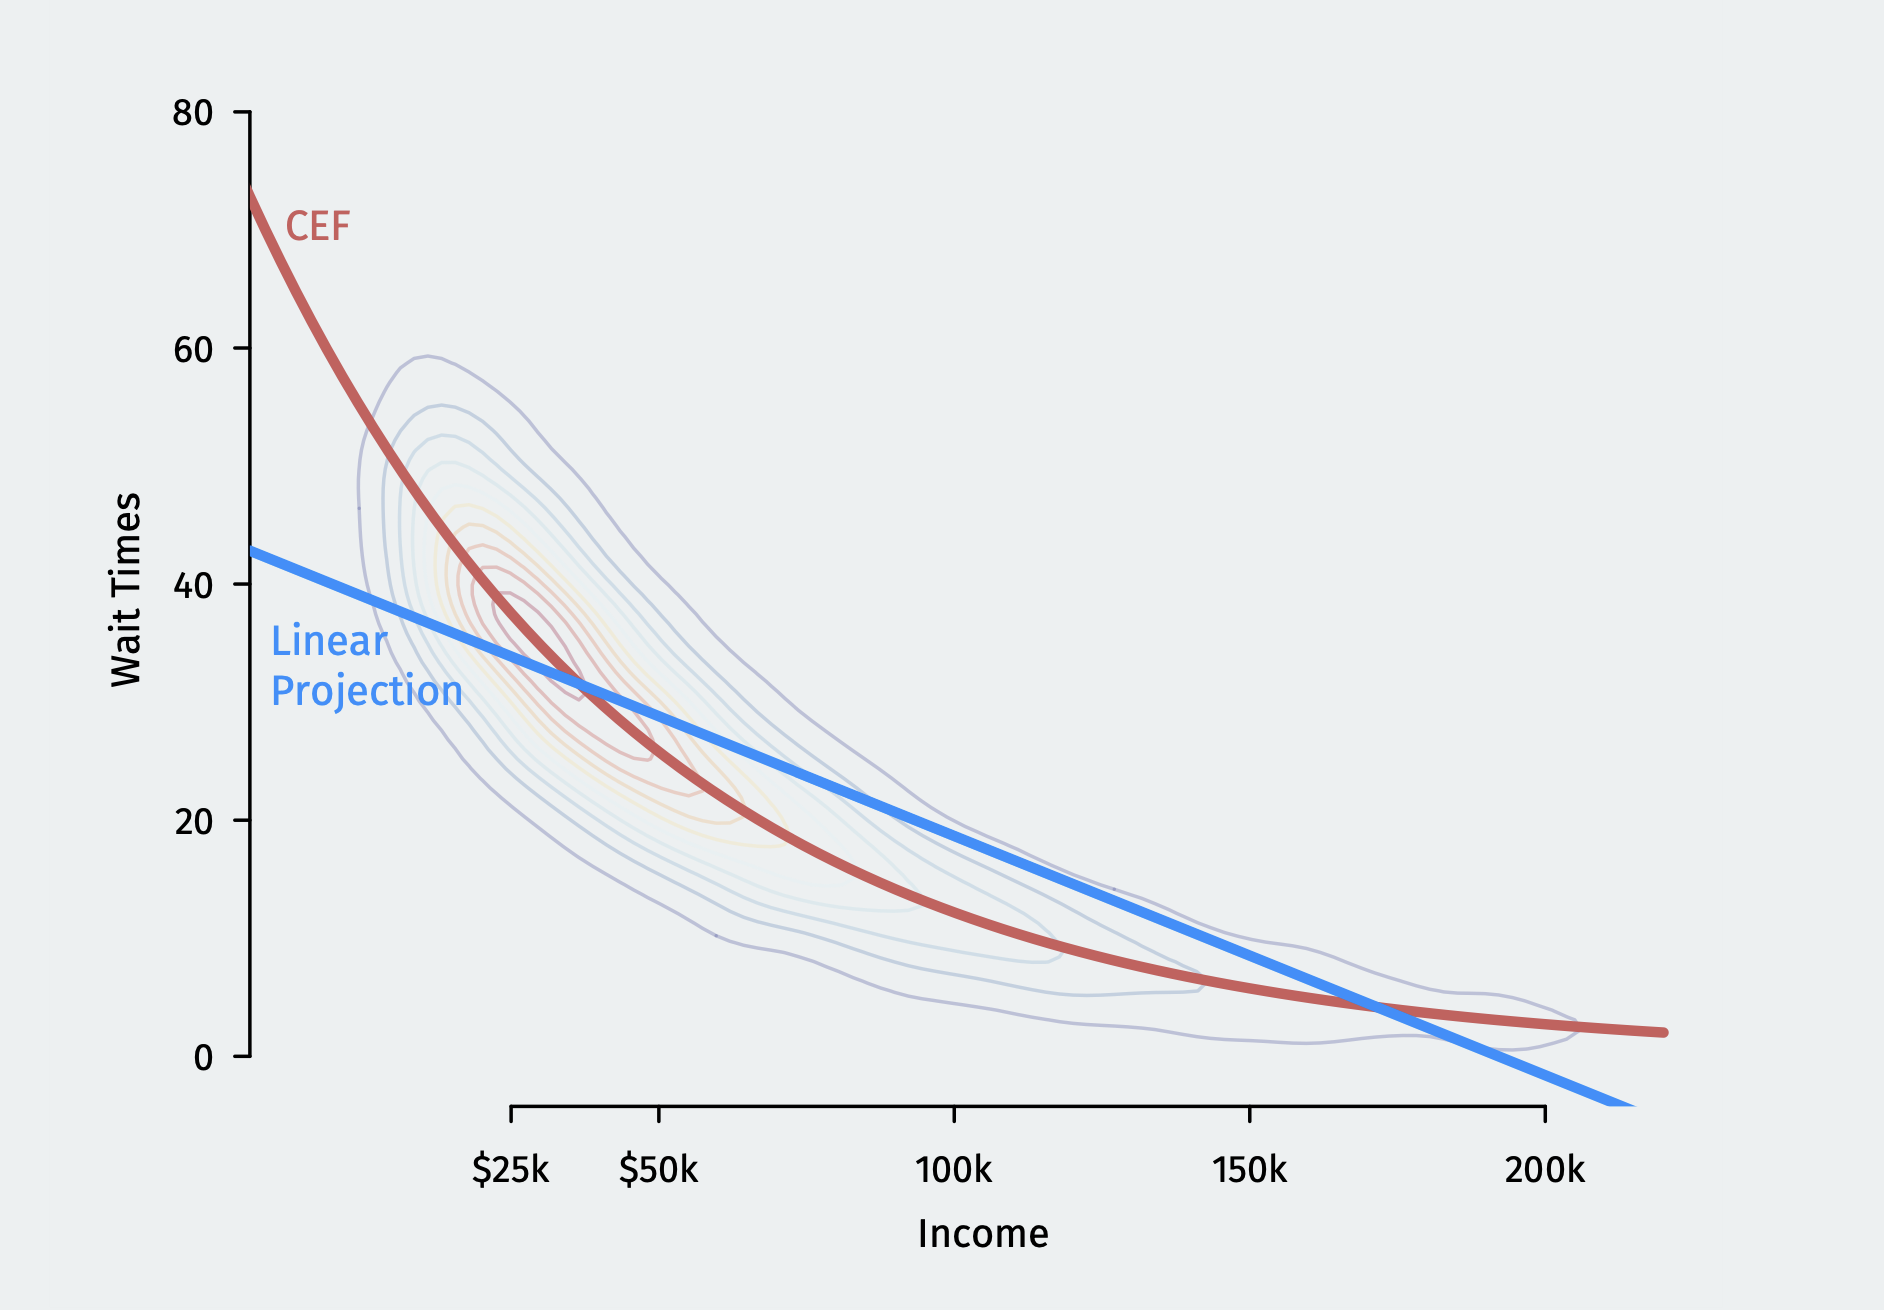
\includegraphics{assets/img/linear-approximation.png}

This book, like many before it, will try to teach you statistics. The
field of statistics describes how we learn about the world using
quantitative data. In the social sciences, an increasing share of
empirical studies use statistical methods to provide evidence for or
against conceptual arguments. And, while it is possible to conduct
quantitative research without understanding statistics at an intuitive
level, it is not a good idea. Quantitative research involves a host of
\emph{choices} about the model to use, variables to include, tuning
parameters to set, assumptions to make, and so on. Without a deep
understanding of statistics, you may find these choices bewildering and
confusing, and you may simply (and possibly erroneously) yield to the
default settings of your statistical software.

The goal of this book is to give you the foundation to make
methodological choices for your specific application with knowledge and
with confidence. The material is intended for first-year PhD students in
political science, but it may be of interest more broadly.

We will focus on two key goals:

\begin{enumerate}
\def\labelenumi{\arabic{enumi}.}
\item
  \textbf{Understand the basic ways to assess estimators} With
  quantitative data, we often want to make statistical inferences about
  some unknown feature of the world. We use estimators (which are just
  ways of summarizing our data) to estimate these features. This book
  will introduce the basics of this task at a general enough level to be
  applicable to almost any estimator that you are likely to encounter in
  empirical research in the social sciences. We will also cover major
  concepts such as bias, sampling variance, consistency, and asymptotic
  normality, which are so common to such a large swath of (frequentist)
  inference that understanding them at a deep level will yield an
  enormous return on your time investment. Once you understand these
  core ideas, you will have a language to analyze any fancy new
  estimator that pops up in the next few decades.
\item
  \textbf{Apply these ideas to the estimation of regression models} This
  book will apply these ideas to one particular social science
  workhorse: regression. Many methods either use regression estimators
  like ordinary least squares or extend them in some way. Understanding
  how these estimators work is vital for conducting research, for
  reading and reviewing contemporary scholarship, and, frankly, for
  being a good and valuable colleague in seminars and workshops.
  Regression and regression estimators also provide an entry point for
  discussing parametric models as approximations, rather than as rigid
  assumptions about the truth of a given specification.
\end{enumerate}

Why write a book on statistics and regression when so many already
exist? While some texts at this level exist in the fields of statistics
and economics, they tend to focus on applications and models less
relevant to other social sciences. This book attempts to correct this.
The book also seeks to introduce a fairly high level of mathematical
sophistication that will challenge and push you to develop stronger
foundations in the material.

\section*{Roadmap}\label{roadmap}
\addcontentsline{toc}{section}{Roadmap}

\markright{Roadmap}

This book has two major parts. Part I introduces the basics of
statistical inference.

We start in Chapter~\ref{sec-design-based} by demonstrating basic
concepts of estimation and inference from the design-based perspective
in which we sample from a fixed, finite population, and all uncertainty
comes from randomness over who is and is not included in the sample.
This framework for inference has deep roots in the statistical
literature and provides a great deal of intuition for how estimation and
uncertainty work in simple settings. We will discuss how to use
design-based inference to estimate features of the population from
samples when the analyst knows the exact sampling design. Unfortunately,
researchers often lack this knowledge about how their data came to be,
limiting the usefulness of this approach.

Chapter~\ref{sec-model-based} introduces a more flexible approach to
estimation: model-based inference. With this approach, the researcher
posits a probability model for how the data came to be. This book
focuses on models that posit ``independent and identically distributed''
data for this model. The chapter describes how estimation and inference
proceed under these models and also introduces a broad class of
estimators based on the plug-in principle.

These two chapters focus on finite sample properties of different
estimation techniques, but we can say more about an estimator if we
consider how it behaves on larger and larger samples.
Chapter~\ref{sec-asymptotics} introduces this type of asymptotic
analysis. It covers the core results of asymptotic theory, such as the
law of large numbers, the central limit theorem, and the delta method,
but also shows why these results are important for statistical
inference. In particular, the chapter shows how these results enable the
creation of asymptotically valid confidence intervals.

Chapter~\ref{sec-hypothesis-tests} wraps up Part I of the book by
introducing statistical inference with hypothesis testing. This chapter
shows how to build hypothesis tests and provides intuition for all their
aspects. We also cover power analyses for planning studies and the
connection between confidence intervals and hypothesis tests.

Part II of the book focuses on one particular estimator of great
importance to quantitative social sciences: the least squares estimator.

Chapter~\ref{sec-regression} begins by describing exactly what quantity
of interest we are targeting when we discuss ``linear models.'' In
particular, we discuss how a population best linear predictor exists
even if the relationship between two variables is nonlinear. This
provides a coherent basis for linear regression estimation as a linear
approximation to a potentially nonlinear function. The chapter also
shows how to interpret the coefficients in these linear regression
models.

Chapter~\ref{sec-ols-mechanics} introduces the more mechanical
properties of the least squares estimator: how the estimator is
constructed, its geometrical interpretation, and how influential
observations may affect the estimates it returns. This chapter
introduces the least squares estimator in matrix form and provides key
intuition for understanding this compact notation.

Finally, Chapter~\ref{sec-ols-statistics} describes the statistical
properties of the least squares estimator. The chapter shows how
modeling assumptions affect the kinds of properties we can obtain. The
weakest modeling assumptions allow us to derive the surprisingly strong
asymptotic properties of least squares that we depend on in most
settings. The chapter then shows how stronger assumptions such as
linearity and normally distributed errors can provide even stronger
results but that they do so at the expense of potential model
misspecification.

\section*{Acknowledgements}\label{acknowledgements}
\addcontentsline{toc}{section}{Acknowledgements}

\markright{Acknowledgements}

Much of how I approach this material comes from Adam Glynn, for whom I
was a teaching fellow during graduate school. Thanks to the students of
Gov 2000 and Gov 2002 over years for helping me refine the material in
this book. Also very special thanks to those who have provided valuable
feedback including Zeki Akyol, Noah Dasanaike, Maya Sen, and Jarell
Cheong Tze Wen.

\section*{Colophon}\label{colophon}
\addcontentsline{toc}{section}{Colophon}

\markright{Colophon}

You can find the source for this book at
\url{https://github.com/mattblackwell/gov2002-book}. Any typos or errors
can be reported at
\url{https://github.com/mattblackwell/gov2002-book/issues}. Thanks for
reading.

This is a Quarto book. To learn more about Quarto books visit
\url{https://quarto.org/docs/books}.

\(\,\) \(\,\)

\part{Statistical Inference}

\chapter{Design-based Inference}\label{sec-design-based}

\section{Introduction}\label{introduction}

Quantitative analysis of social data has an alluring exactness to it. It
allows us to estimate the average number of minutes of YouTube videos
watched to the millisecond, and in doing so it gives us the aura of true
scientists. But the advantage of quantitative analyses lies not in the
ability to derive precise three-decimal point estimates; rather,
quantitative methods shine because they allow us to communicate
methodological goals, assumptions, and results in a (hopefully) common,
compact, and precise mathematical language. It is this language that
helps clarify \emph{exactly} what researchers are doing with their data
and why.

This dewy view of quantitative methods is unfortunately often at odds
with how these methods are used in the real world. All too often we as
researchers find some arbitrary data, apply a statistical tool with
which we are familiar, and then shoehorn the results into a theoretical
story that may or may not have a (tenuous) connection. Quantitative
methods applied this way will provide us with a very specific answer to
a murky question about a shapeless target.

This book is a guide to a better foundation for quantitative analysis
and, in particular, for statistical inference. Inference is the task of
using the data we have to learn something about the data we do not have.

The organizing motto of this book is to help us as researchers be

\begin{quote}
Precise in stating our goals, transparent in stating our assumptions,
and honest in evaluating our results.
\end{quote}

These goals are the target of our inference -- or what do we want to
learn and about whom.

In pursuing these goals, this book will focus on a general workflow for
statistical inference. The workflow boils down to answering a series of
questions about the goals, assumptions, and methods of our analysis:

\begin{enumerate}
\def\labelenumi{\arabic{enumi}.}
\tightlist
\item
  \textbf{Population}: who or what do we want to learn about?
\item
  \textbf{Design/model}: how will we collect the data, or, what
  assumptions are we making about how the data came to be?
\item
  \textbf{Quantity of Interest}: what do we want to learn about the
  population?\\
\item
  \textbf{Estimator}: how will we use the data to produce an estimate?
\item
  \textbf{Uncertainty}: how will we estimate and convey the error
  associated with the estimate?
\end{enumerate}

These questions form the core of any quantitative research endeavor. And
the answers to these will draw on a mixture of substantive interests,
feasibility, and statistical theory, and this mixture will vary from
question to question. For example, the population of interest can vary
greatly from study to study, whereas many disparate studies may employ
the same estimand and estimator.

The third core question is particularly important, since it highlights
an essential division in how researchers approach statistical inference
-- specifically, \textbf{design-based inference} vs \textbf{model-based
inference}. Design-based inference typically focuses on situations in
which we have precise knowledge of how our sample was randomly selected
from the population. Uncertainty here comes exclusively from the random
nature of which observations are included in the sample. By contrast, in
the \textbf{model-based} framework, we treat our data as random
variables and propose a probabilistic model for how the data came to
exist. The models then vary in the strength of their assumptions.

Design-based inference is the framework that addresses the core
inferential questions most crisply, and so it is the focus of this
chapter. Its main disadvantages are that it is considerably less general
than the model-based approach and that the mathematics of the framework
are slightly more complicated.

We will now go over each of the core questions in more detail.

\section{Question 1: Population}\label{question-1-population}

Inference is the task of using the data that we have to learn facts
about the world (i.e., the data we do not have). The most
straightforward setting is when we have a fixed set of units that we
want to learn something about. These units are what we call the
\textbf{population} or \textbf{target population}. We are going to focus
on random sampling from this population, but, to do so, we need to have
a list of units from the population. This list of \(N\) units is called
the \textbf{frame} or \textbf{sampling frame}, and we will index these
units in the sampling frame by \(i \in \mathcal{U} = \{1, \ldots, N\}\).
Here we assume that \(N\), the size of the population, is known, but
note that this may not always be true.

The sampling frame may differ from the target population simply for
feasibility reasons. For example, the target population might include
all the households in a given city, but the sampling frame might be the
list of all residential telephone numbers for that city. Of course, many
households do not have landline telephones and rely on mobile phone
exclusively. This gap between the target population and the sampling
frame is called \textbf{undercoverage} or \textbf{coverage bias}.

\begin{example}[]\protect\hypertarget{exm-frame-bias}{}\label{exm-frame-bias}

An early but prominent example of frame bias in survey sampling is the
infamous \emph{Literary Digest} poll of the 1936 U.S. presidential
election. \emph{Literary Digest}, a (now defunct) magazine, sent over 10
million ballots to addresses found in automobile registration lists and
telephone books, trying to figure out who would win the important 1936
presidential race. The sample size was huge: over 2 million respondents.
In the end, the results predicted that Alf Landon, the Republican
candidate, would receive 55\% of the vote, while the incumbent,
Democratic President Franklin D. Roosevelt, would only win 41\% of the
vote. Unfortunately for the \emph{Literary Digest}, Landon only received
37\% of the vote.

There are many possible reasons for this massive polling error. Most
obviously, the sampling frame was different from that of the target
population. Why? Only those with either a car or a telephone were
included in the sampling frame, and people without either overwhelmingly
supported the Democrat, Roosevelt. While this is not the only source of
bias -- differential nonresponse seems to be a particularly big problem
--the frame bias contributes a large part of the error. For more about
this poll, see SQUIRE (1988).

\end{example}

One advantage of design-based inference is how precisely we must
articulate the sampling frame. We can be extremely clear about the group
of units we are trying to learn about. We shall see that in model-based
inference the concept of the population and sampling frame become more
amorphous.

\begin{example}[American National Election Survey,
Population]\protect\hypertarget{exm-anes-population}{}\label{exm-anes-population}

According to the materials from the American National Election Survey
(ANES) in 2012, its target population is all U.S. citizens age 18 or
older. The sampling frame for the face-to-face portion of the survey
``consisted of the Delivery Sequence File (DSF) used by the United
States Postal Service'' for residential delivery of mail.''
Unfortunately, there are housing units that are covered by mail delivery
by the postal service which would result in the potential for frame
bias. The designers of the ANES used the Decennial Census to add many of
these units to the final sampling frame.

\end{example}

\section{Question 2: Sampling design}\label{question-2-sampling-design}

Now that we have a clearly defined population and sampling frame, we can
consider how to select a sample from the population. We will focus on
\textbf{probabilistic samples}, where units are selected into the sample
by chance, and each unit in the sampling frame has a non-0 probability
of being included. Let \(\mathcal{S} \subset \mathcal{U}\) be a sample
and let \(\mb{Z} = (Z_1, Z_2, \ldots, Z_N)\) to be a vector of inclusion
indicators such that \(Z_i = 1\) if \(i \in \mathcal{S}\) and
\(Z_i = 0\) otherwise. We denote these indicators as upper-case letters
because they are random variables. We assume the sample size is
\(|\mathcal{S}| = n\).

Suppose our sampling frame was the hobbits who are members of the
Fellowship of the Ring, an exclusive group brought into being by a
wizened elf lord. This group of four hobbits is a valid -- albeit small
and fictional population -- with \(\mathcal{U} =\) \{Frodo, Sam, Pip,
Merry\}.

Suppose we want to sample two hobbits from this group. We can list all
six possible samples of size two from this population in terms of the
sample members \(\mathcal{S}\) or, equivalently, the inclusion
indicators \(\mb{Z}\):

\begin{itemize}
\tightlist
\item
  \(\mathcal{S}_1 =\) \{Frodo, Sam\} with \(\mb{Z}_{1} = (1, 1, 0, 0)\)
\item
  \(\mathcal{S}_2 =\) \{Frodo, Pip\} with \(\mb{Z}_{2} = (1, 0, 1, 0)\)
\item
  \(\mathcal{S}_3 =\) \{Frodo, Merry\} with
  \(\mb{Z}_{3} = (1, 0, 0, 1)\)
\item
  \(\mathcal{S}_4 =\) \{Sam, Pip\} with \(\mb{Z}_{4} = (0, 1, 1, 0)\)
\item
  \(\mathcal{S}_5 =\) \{Sam, Merry\} with \(\mb{Z}_{5} = (0, 1, 0, 1)\)
\item
  \(\mathcal{S}_6 =\) \{Pip, Merry\} with \(\mb{Z}_{6} = (0, 0, 1, 1)\)
\end{itemize}

A \textbf{sampling design} is a complete specification of how likely to
be selected each of these samples is. That is, we need to determine a
selection probability \(\pi_j\) for each sample \(\mathcal{S}_j\). The
most widely used and widely studied design is one that places equal
probability on each of the possible samples of size \(n\).

\begin{definition}[]\protect\hypertarget{def-srs}{}\label{def-srs}

A \textbf{simple random sample} (srs) is a probability sampling design
where each possible sample of size \(n\) has the same probability of
occurring. More specifically, let \(\mb{z} = (z_{1}, \ldots, z_{N})\) be
a particular possible sampling, then, \[
\P(\mb{Z} = \mb{z}) = \begin{cases}
{N \choose n}^{-1} &\text{if } \sum_{i=1}^N z_i = n,\\
0 & \text{otherwise}
\end{cases}
\]

\end{definition}

If we sampled two hobbits, the srs (the simple random sample) would
place \(1/{4\choose 2} = 1/6\) probability of each of the above samples
\(\mathcal{S}_j\). Note that the srs gives zero probability to any
sample that does not have exactly \(n\) units in the sample.

Another common sampling design --the \textbf{Bernoulli sampling} design
-- works by choosing each unit independently with the same probability.

\begin{definition}[]\protect\hypertarget{def-srs}{}\label{def-srs}

\textbf{Bernoulli sampling} is a probability sampling design where
independent Bernoulli trials with probability of success \(q\) determine
whether each unit in the population will be included in the sample. More
specifically, let \(\mb{z} = (z_{1}, \ldots, z_{N})\) be a particular
possible sampling. Bernoulli sampling will then be \[
\P(\mb{Z} = \mb{z}) = \P(Z_1 = z_1) \cdots \P(Z_N = z_N) = \prod_{i=1}^N q_i^{Z_i}(1 - q_i)^{1-Z_i}
\]

\end{definition}

Bernoulli sampling is very straightforward because independently
selecting units simplifies many calculations. However, this ``coin
flipping'' approach means that the sample size,
\(N_s = \sum_{i=1}^N Z_i\), will be itself a random variable because it
is the result of how many of the coin flips land on ``heads.''

Simple random samples and Bernoulli random samples are simple to
understand and implement. For large surveys, the sampling designs are
often much more complicated for cost-saving reasons. We now describe the
sampling design for the ANES, which contains many design features
typical of similar large surveys.

\begin{example}[American National Election Survey, Sampling
Design]\protect\hypertarget{exm-anes-design}{}\label{exm-anes-design}

The ANES uses a typical yet complicated design for its 2012 face-to-face
survey. First, the designers divided (or stratified) U.S. states into
nine Census divisions (which are based on geography). Within each
division, designers then randomly sampled a number of census tracts
(with higher number of sampled tracts for divisions with higher
populations). The census tracts with larger populations are selected
with higher probability.

The second stage randomly samples addresses from the sampling frame
(described in Example~\ref{exm-anes-population}). More households were
sampled from tracts with higher proportion of Black and Latino residents
to obtain an oversample of these groups.

Finally, the third stage of sampling was to randomly select one eligible
person per household for completion of the survey.

\end{example}

\section{Question 3: Quantity of
Interest}\label{question-3-quantity-of-interest}

The \textbf{quantity of interest} is a numerical summary of the
population that we want to learn about. These quantities are also called
\textbf{estimands} ( Latin for ``the thing to be estimated'').

Let \(x_1, x_2, \ldots, x_N\) be a fixed set of characteristics, or
items, about the population. Using the statistician's favorite home
decor, we might think about our population as a set of marbles in a jar
where the \(x_i\) values indicate, for example, the color of the
\(i\)-th marble. In a survey, \(x_i\) might represent the age, ideology,
or income of the \(i\)-th person in the population.

We can define many useful quantities of interest based on the population
characteristics. These quantities generally summarize the values
\(x_1, \ldots, x_N\). One of the most common, and certainly one of the
most useful, is the \textbf{population mean}, defined as \[
\overline{x} = \frac{1}{N} \sum_{i=1}^N x_i.
\] The population mean is fixed because \(N\) and the population
characteristics \(x_1, \ldots, x_N\) are fixed. Another common estimand
in the survey sampling literature is the population total, \[
t = \sum_{i=1}^N x_i = N\overline{x}.
\]

\begin{example}[Subpopulation
means]\protect\hypertarget{exm-subpopulation}{}\label{exm-subpopulation}

We may also be interested in quantities for different subdomains.
Suppose we are interested in estimating the fraction of (say)
conservative-identifying respondents who support increasing legal
immigration. Let \(d= 1, \ldots, D\) be the number of subdomains or
subpopulations. In this case, we might have \(d = 1\) as liberal
identifiers, \(d = 2\) as moderate identifiers, and \(d = 3\) as
conservative identifiers. We will refer to the subpopulation for each of
these groups as \(\mathcal{U}_d \subset \{1,\ldots, N\}\) and we define
the size of these groups as \(N_d = |\mathcal{U}_d\). So, \(N_3\) would
be the number of conservative-identifying citizens in the population.

The mean for each group is then \[
\overline{x}_d = \frac{1}{N_d} \sum_{i \in \mathcal{U}_d} x_i.
\]

Subpopulation estimation can be slightly more complicated than
population estimation because we may not know who is in which
subpopulation until we actually sample the population. For example, our
sampling frame probably may not information about `potential
respondents' ideology. Thus, \(N_d\) will be unknown to the researcher,
unlike \(N\) for the population mean, which is known.

\end{example}

We may be interested in many other quantities of interest, but
design-based inference is largely focused on these types of population
and subpopulation means and totals.

\section{Question 4: Estimator}\label{question-4-estimator}

Now that we have a sampling design and a quantity of interest, we can
consider what we can learn about this quantity of interest from our
sample. An \textbf{estimator} is a function of the sample measurements
intended as a best guess about our quantity of interest.

If the most common estimand is the population mean, the most popular
estimator is the \textbf{sample mean}, defined as \[
\overline{X}_n = \frac{1}{n} \sum_{i=1}^{N}Z_ix_i
\]

The sample mean is a \textbf{random} quantity since it varies from
sample to sample, and those samples are chosen probabilistically. For
example, suppose we have height measurements from our small population
of hobbits in Table~\ref{tbl-hobbit-pop}.

\begin{longtable}[]{@{}ll@{}}
\caption{A small population of
hobbits}\label{tbl-hobbit-pop}\tabularnewline
\toprule\noalign{}
Unit (\(i\)) & Height in cm (\(x_i\)) \\
\midrule\noalign{}
\endfirsthead
\toprule\noalign{}
Unit (\(i\)) & Height in cm (\(x_i\)) \\
\midrule\noalign{}
\endhead
\bottomrule\noalign{}
\endlastfoot
1 (Frodo) & 124 \\
2 (Sam) & 127 \\
3 (Pip) & 123 \\
4 (Merry) & 127 \\
\end{longtable}

If we consider a simple random sample of size \(n=2\) from this
population, we can list the probability of all possible sample means
associated with this sampling design as we do in
Table~\ref{tbl-hobbit-samples}. Table~\ref{tbl-sampling-dist} combines
the equivalent values of the sample mean to arrive at the
\textbf{sampling distribution} of the sample mean of hobbit height under
a srs of size 2.

\begin{longtable}[]{@{}
  >{\raggedright\arraybackslash}p{(\columnwidth - 4\tabcolsep) * \real{0.2466}}
  >{\raggedright\arraybackslash}p{(\columnwidth - 4\tabcolsep) * \real{0.3151}}
  >{\raggedright\arraybackslash}p{(\columnwidth - 4\tabcolsep) * \real{0.4384}}@{}}
\caption{All possible simple random samples of size 2 from the hobbit
population}\label{tbl-hobbit-samples}\tabularnewline
\toprule\noalign{}
\begin{minipage}[b]{\linewidth}\raggedright
Sample (\(j\))
\end{minipage} & \begin{minipage}[b]{\linewidth}\raggedright
Probability (\(\pi_j\))
\end{minipage} & \begin{minipage}[b]{\linewidth}\raggedright
Sample mean (\(\overline{X}_n\))
\end{minipage} \\
\midrule\noalign{}
\endfirsthead
\toprule\noalign{}
\begin{minipage}[b]{\linewidth}\raggedright
Sample (\(j\))
\end{minipage} & \begin{minipage}[b]{\linewidth}\raggedright
Probability (\(\pi_j\))
\end{minipage} & \begin{minipage}[b]{\linewidth}\raggedright
Sample mean (\(\overline{X}_n\))
\end{minipage} \\
\midrule\noalign{}
\endhead
\bottomrule\noalign{}
\endlastfoot
1 (Frodo, Sam) & 1/6 & (124 + 127) / 2 = 125.5 \\
2 (Frodo, Pip) & 1/6 & (124 + 123) / 2 = 123.5 \\
3 (Frodo, Merry) & 1/6 & (124 + 127) / 2 = 125.5 \\
4 (Sam, Pip) & 1/6 & (127 + 123) / 2 = 125 \\
5 (Sam, Merry) & 1/6 & (127 + 127) / 2 = 127 \\
6 (Pip, Merry) & 1/6 & (123 + 127) / 2 = 125 \\
\end{longtable}

\begin{longtable}[]{@{}ll@{}}
\caption{Sampling distribution of the sample mean for simple random
samples of size 2 from the hobbit
population}\label{tbl-sampling-dist}\tabularnewline
\toprule\noalign{}
Sample mean & Probability \\
\midrule\noalign{}
\endfirsthead
\toprule\noalign{}
Sample mean & Probability \\
\midrule\noalign{}
\endhead
\bottomrule\noalign{}
\endlastfoot
123.5 & 1/6 \\
125 & 1/3 \\
125.5 & 1/3 \\
127 & 1/6 \\
\end{longtable}

Thus, the sampling distribution tells us what values of an estimator are
more or less likely and depends on both the population distribution and
the sampling design.

\begin{tcolorbox}[enhanced jigsaw, toptitle=1mm, bottomrule=.15mm, leftrule=.75mm, rightrule=.15mm, breakable, colframe=quarto-callout-note-color-frame, title=\textcolor{quarto-callout-note-color}{\faInfo}\hspace{0.5em}{Note}, colbacktitle=quarto-callout-note-color!10!white, titlerule=0mm, coltitle=black, left=2mm, colback=white, bottomtitle=1mm, opacitybacktitle=0.6, opacityback=0, toprule=.15mm, arc=.35mm]

Notice that the sampling distribution of an estimator will depend on the
sampling design. Here, we used a simple random sample. Bernoulli
sampling would have produced a different distribution. Using Bernoulli
sampling, we could end up with a sample of just Frodo, in which case the
sample mean would be his height (124cm), a sample mean value that is
impossible with simple random sampling of size \(n=2\).

\end{tcolorbox}

\subsection{Properties of the sampling distribution of an
estimator}\label{properties-of-the-sampling-distribution-of-an-estimator}

Generally speaking, we want ``good'' estimators. But what makes an
estimator ``good'\,'? The best estimator would obviously be the one that
is right all of the time (\(\Xbar_n = \overline{x}\) with probability
1), but this is only possible if we conduct a census --that is, sample
everyone in the population -- or the population does not vary. Neither
situation is typical for most researchers.

We instead focus on properties of the sampling distribution of an
estimator. The following types of questions get at these properties:

\begin{itemize}
\tightlist
\item
  Are the estimator's observed values (realizations) centered on the
  true value of the quantity of interest? (unbiasedness)
\item
  Is there a lot or a little variation in the realizations of the
  estimator across different samples from the population? (sample
  variance)
\item
  On average, how close to the truth is the estimator? (mean square
  error)
\end{itemize}

The answers to these questions will depend on (a) the estimator and (b)
the sampling design.

To back up, the sampling distribution shows us all the possible values
of an estimator across different samples from the population. If we want
to summarize this distribution with a single number, we would focus on
its expectation, which is a measure of central tendency of the
distribution. Roughly speaking, we want the center of the distribution
to be close to and ideally equal to the true quantity of interest. If
this is not the case, that means the estimator systematically over- or
under-estimates the truth. We call this difference the \textbf{bias} of
an estimator, which can be written mathematically as \[
\textsf{bias}[\Xbar_{n}] = \E[\Xbar_{n}] - \overline{x}.
\] Any estimator that has bias equal to zero is call an
\textbf{unbiased} estimator.

We can calculate the bias of our hobbit srs (where we sampled two
hobbits from the Fellowship of the Ring with equal probability) by first
calculating the expected value of the estimator, \[
\E[\Xbar_{n}] = \frac{1}{6}\cdot 123.5 + \frac{1}{3} \cdot 125 + \frac{1}{3} \cdot 125.5 + \frac{1}{6} \cdot 127 = 125.25,
\] and comparing this to the population mean, \[
\overline{x} = \frac{1}{4}\left(124 + 127 + 123 + 127\right) = 125.25.
\] The two are the same, meaning the sample mean in this simple random
sample is unbiased.

\begin{tcolorbox}[enhanced jigsaw, toptitle=1mm, bottomrule=.15mm, leftrule=.75mm, rightrule=.15mm, breakable, colframe=quarto-callout-warning-color-frame, title=\textcolor{quarto-callout-warning-color}{\faExclamationTriangle}\hspace{0.5em}{Warning}, colbacktitle=quarto-callout-warning-color!10!white, titlerule=0mm, coltitle=black, left=2mm, colback=white, bottomtitle=1mm, opacitybacktitle=0.6, opacityback=0, toprule=.15mm, arc=.35mm]

Note that the word ``bias'' sometimes also refers to research that is
systematically incorrect in other ways. For example, we might complain
that a survey question is biased if it presents a leading or misleading
question or if it mismeasures the concept of interest. To see this,
suppose we wanted to estimate the proportion of a population that
regularly donates money to a political campaign, but \(x_i\) actually
measures whether a person donated on the day of the survey. In this
case, \(\overline{x}\) would be quite a bit lower than the quantity of
interest because it only captures one day of donation patterns, not
regular donations made over time. Textbooks often refer to this gap
between the measures we obtain and the measures we want as
\textbf{measurement bias}. This is distinct from the bias of the sample
mean. Using our donations example, taking an srs from the population of
daily donors, \(\Xbar_{n}\) would still result in an unbiased estimate
for \(\overline{x}\), even if that is entirely the wrong quantity of
interest.

\end{tcolorbox}

Is the unbiasedness of our hobbit sampling unique to this example?
Thankfully no. We can prove that the sample mean will be unbiased for
the population mean under a simple random sample. Relying on the
definition of the sample mean, we can obtain: \[ 
\E[\Xbar_{n}] = \E\left[\frac{1}{n} \sum_{i=1}^{N} Z_{i}x_{i}\right] = \frac{1}{n} \sum_{i=1}^{N} \E[Z_{i}]x_{i} = \frac{1}{n} \sum_{i=1}^{N} \frac{n}{N}x_{i} = \frac{1}{N} \sum_{i=1}^{N}x_{i} = \overline{x} 
\] Using \(\E[Z_i] = n/N\) for the simple random sample in the second
equality is key. Intuitively, the probability of being included in the
sample is simply the fraction of the sample being selected, \(n/N\).

The second salient feature of an estimator's sampling distribution is
its spread. Generally speaking, we prefer an estimator whose estimates
are very similar from sample to sample over an estimator whose estimates
vary wildly from one sample to the next. We quantify this spread with
the \textbf{sampling variance}, which is simply the variance of the
sampling distribution of the estimator, or \[
\V[\Xbar_n] = \E[(\Xbar_n - \E[\Xbar_n])^2].
\] An alternative measure of spread is the \textbf{standard error} of
the estimator, which is the square root of the sampling variance, \[
\se[\Xbar_n] = \sqrt{\V[\Xbar_n]}.
\] The standard error is often more interpretable because it is on the
same scale as the original variable. Using our hobbits' heights example,
the sampling variance would be measured in centimeters squared but the
standard error would be measured in centimeters and, thus, easier to
interpret.

The final important property is the \textbf{mean squared error} or
\textbf{MSE}, which (as its name implies) measures the average of the
squared error: \[
\text{MSE} = \E[(\Xbar_n-\overline{x})^2].
\] Keen-eyed readers might find this quantity redundant because, as we
showed above, the sample mean is unbiased, so
\(\E[\Xbar_n] = \overline{x}\). This, in turn, means that the sampling
variance of the sample mean is just the mean squared error. However,
circumstances will often conspire to make us use biased estimators, so
these two quantities will differ. In fact, if we have an estimator
\(\widehat{\theta}\) for some population quantity \(\theta\), \[ 
\begin{aligned}
\text{MSE}[\widehat{\theta}] &= \E[(\widehat{\theta} - \theta)^2] \\
&= \E[(\widehat{\theta} - \E[\widehat{\theta}] + \E[\widehat{\theta}] - \theta)^2] \\
&= \E[(\widehat{\theta} - \E[\widehat{\theta}])^2] + \left(\E[\widehat{\theta}] - \theta\right) ^ 2 + 2\E[(\widehat{\theta} - \E[\widehat{\theta}])]\left(\E[\widehat{\theta}] - \theta\right) \\
&= \text{bias}[\widehat{\theta}_n]^2 + \V[\widehat{\theta}_n]  
\end{aligned}
\] Thus, the MSE is low when bias and variance are low.

Note that connecting these concepts to notions of precision and accuracy
is useful. In particular, estimators with low sampling variance are
\textbf{precise}, whereas estimators with low MSE are \textbf{accurate}.
An estimator can be very precise, but the same estimator can be
inaccurate because it is biased.

\section{Question 5: Uncertainty}\label{question-5-uncertainty}

We now have a population, a quantity of interest, a sampling design, an
estimator, and, with data, an actual estimate. But if we sampled, say,
Sam and Merry from the hobbit population and obtained a sample mean
height of 127, a reasonable worry would be that different samples -- for
example, Sam and Frodo or Merry and Pippin -- would give us a different
sample mean. So is the estimate of 127 inches that we get from our
sample of Sam and Merry close to the true population mean? We cannot
truly know without conducting a complete census of all four hobbits,
which would render our sampling pointless. Can we instead figure out how
far we might be from the truth -- i.e., the true population mean? The
sampling variance addresses this exact question, but the sampling
variance depends on the sampling distribution, and we only have a single
sample draw from this distribution, which gave the estimate of 127.

If we have a specific estimator and a sampling design, we can usually
derive an analytical expression for the sampling variance (and, thus,
the standard error), which in turn will identify the factors influencing
the sampling variance. To aid in this endeavor, we need to define an
additional feature of the population distribution, the
\textbf{population variance}, \[
s^{2}= \frac{1}{N-1} \sum_{i=1}^{N} (x_{i} - \overline{x})^{2}.
\] The population variance measures the spread of the \(x_i\) values in
the population. As such it is a fixed quantity and not a random
variable.

We now write the sampling variance of \(\Xbar_n\) under simple random
sampling as \[
\V[\Xbar_{n}] = \left(1 - \frac{n}{N}\right) \frac{s^{2}}{n}
\] Several features stand out from this expression. First, if the data
\(x_i\) is more spread out in the population, the sample mean will also
be more spread out. Second, the larger the sample size, \(n\), the
smaller the sampling variance (for a fixed population size). Third, the
larger the population size, \(N\), the smaller the sampling variance
(again for a fixed sample size).

\subsection{Deriving the sampling variance of the sample
mean}\label{deriving-the-sampling-variance-of-the-sample-mean}

How did we obtain this expression for the sampling variance under simple
random sampling? It would be tempting to simply say ``someone else
proved it for me,'' but blind faith in statistical theory limits our own
understanding of this situation and the ability to navigate novel
scenarios that routinely arise in research.

To derive the sampling variance of the sample mean, let's begin with a
simple application of the rules of variance that would be valid for any
sampling design: \[
\V[\Xbar_{n}] = \V\left[\frac{1}{n} \sum_{i=1}^N x_iZ_i\right] = \frac{1}{n^2}\left[\sum_{i=1}^N x_i^2\V[Z_i] + \sum_{i=1}^N\sum_{j\neq i} x_ix_j\cov[Z_i,Z_j]\right].
\] Note in the second equality that the \(x_i\) and \(x_j\) values come
out of the variance and covariance operators as if they are constants.
This is because, in design-based inference, they are exactly constants.
The only source of variation and uncertainty comes from the sampling,
indicated by the inclusion indicators, \(Z_i\). To make progress, we
need to know the variance and covariance of these inclusion indicators.
Recall that the variance of a binary indicator with probability \(p\) of
being 1 is \(p(1 - p)\). So if \(\P(Z_i = 1) = n/N\) for a simple random
sample, then \[
\V[Z_i] = \frac{n}{N}\left(1 - \frac{n}{N}\right) = \frac{n(N - n)}{N^2}.
\]

If you are used to the ``independent and identically distributed''
framework (to which we will turn in the next chapter), the covariances
in the sampling variances might surprise. Aren't units usually assumed
to be independent? While this assumption would (and will) make our math
lives easier, it is not true for the simple random sample. The srs
samples units without replacement, which implies that units' inclusion
into the sample is not independent---knowing that unit \(i\) was
included in the sample means that another unit \(j\) has only a
\((n-1)/(N-1)\) probability of being included in the sample. To derive
an expression for the covariance, note that
\(\cov(Z_i, Z_j) = \E[Z_iZ_j] - \E[Z_i]\E[Z_j]\) and \[
\E[Z_iZ_j] = \P(Z_i = 1, Z_j = 1) = \P(Z_i = 1)\P(Z_j =1 \mid Z_i = 1) = \frac{n}{N}\cdot \frac{n-1}{N-1}.
\] Plugging this into our covariance statement, we get \[
\begin{aligned}
\cov(Z_i, Z_j) &= \E[Z_iZ_j] - \E[Z_i]\E[Z_j] \\ &= \frac{n}{N}\cdot \frac{n-1}{N-1} - \frac{n^2}{N^2}. \\
&=\frac{n}{N}\left(\frac{n-1}{N-1} - \frac{n}{N}\right) \\
&= \frac{n}{N}\left(\frac{Nn-N - Nn + n}{N(N-1)}\right) \\
&= -\frac{n(N- n)}{N^2(N-1)} \\
&= -\frac{\V[Z_i]}{N-1}.
\end{aligned}
\] Given that variances and population sizes must be positive, the
covariance between the inclusions of two units is negative. Going back
to our hobbits, there are a fixed number of spots in the sample, and so
Frodo being included lowers the chance that Sam is included, so we end
up with this negative covariance.

With the covariance and variance now calculated, we can derive the
sampling variance of the sample mean: \[
\begin{aligned}
\V[\Xbar_{n}] &=  \frac{1}{n^2}\left[\sum_{i=1}^N x_i^2\V[Z_i] + \sum_{i=1}^N\sum_{j\neq i} x_ix_j\cov[Z_i,Z_j]\right] \\
&=  \frac{1}{n^2}\left[\sum_{i=1}^N x_i^2\V[Z_i] - \frac{1}{N-1} \sum_{i=1}^N\sum_{j\neq i} x_ix_j\V[Z_i]\right] \\
&=  \frac{\V[Z_i]}{n^2}\left[\sum_{i=1}^N x_i^2 - \frac{1}{N-1} \sum_{i=1}^N\sum_{j\neq i} x_ix_j\right] \\
&=  \frac{N-n}{nN^2}\left[\sum_{i=1}^N x_i^2 - \frac{1}{N-1} \sum_{i=1}^N\sum_{j\neq i} x_ix_j\right]
\end{aligned}
\] Where do we go from here? Unfortunately, we have arrived at the
non-obvious and seemingly magical step of ``adding and subtracting a
crucial quantity.'' (One needs to know the step before completing the
proof, so how could you complete the proof without knowing this step?)
In this case, it is necessary to add and subtract the quantity
\((N-1)^{-1} \sum_{i=1}^N x_i^2\). To see why, rewrite the population
variance in a slightly different way: \[
s^2 = \frac{1}{N-1}\sum_{i=1}^N (x_i - \overline{x})^2 = \frac{1}{N-1} \left(\sum_{i=1}^N x_i^2  - N\overline{x}^2\right)
\] Note that we can write \[
N^2\overline{x}^2 = \sum_{i=1}^N x_i^2 + \sum_{i=1}^N \sum_{j\neq i} x_ix_j, 
\] which provides a hint as to the quantity that we will add and
subtract \[
\begin{aligned}
\V[\Xbar_{n}] &=  \frac{N-n}{nN^2}\left[\sum_{i=1}^N x_i^2  \textcolor{red!50}{\underbrace{+ \frac{1}{N-1}\sum_{i=1}^N x_i^2 - \frac{1}{N-1}\sum_{i=1}^N x_i^2}_{\text{add and subtract}}} - \frac{1}{N-1} \sum_{i=1}^N\sum_{j\neq i} x_ix_j\right] \\
&=  \frac{N-n}{nN^2}\left[\frac{N}{N-1}\sum_{i=1}^N x_i^2  - \frac{1}{N-1} \sum_{i=1}^N\sum_{j=i}^N x_ix_j\right] \\
&=  \frac{N-n}{nN^2}\left[\frac{N}{N-1}\sum_{i=1}^N x_i^2  - \frac{N^2}{N-1} \overline{x}\right] \\
&=  \frac{N-n}{nN(N-1)}\left[\sum_{i=1}^N x_i^2  - N \overline{x}\right] \\
&=  \frac{N-n}{nN(N-1)}\sum_{i=1}^N (x_i - \overline{x})^2 \\
&= \frac{(N-n)}{N}\frac{s^2}{n} = \left(1 - \frac{n}{N}\right)\frac{s^2}{n}.
\end{aligned}
\] This proof is rather involved but does display some commonly used
approaches to deriving statistical results. It also highlights how the
sampling scheme leads to dependence, making the result more complicated.
The next chapter will discuss how the variance of the sample mean under
independent and identically distributed sampling is much simpler.

\subsection{Estimating the sampling
variance}\label{estimating-the-sampling-variance}

An unfortunate aspect of the sampling variance, \(\V[\Xbar_n]\), is that
it depends on the population variance, \(s^2\), which we cannot know
unless we have a census of the entire population (If we had that
information, we would not need to worry about uncertainty.) Thus, we
need to estimate the sampling variance. Since we already know \(n\), the
sample size, and \(N\), the population size, the most straightforward
way to do this is to find an estimator for the population variance.

A good estimator for this is the \textbf{sample variance}, which is
simply the variance formula applied to the sample itself, \[
S^2 = \frac{1}{n-1} \sum_{i=1}^N Z_i(x_i - \Xbar_n)^2.
\] We can obtain an estimator for the sampling variance by substituting
this in for the population variance, \[
\widehat{\V}[\Xbar_n] = \left(1 - \frac{n}{N}\right)\frac{S^2}{n}.
\]

\begin{tcolorbox}[enhanced jigsaw, toptitle=1mm, bottomrule=.15mm, leftrule=.75mm, rightrule=.15mm, breakable, colframe=quarto-callout-warning-color-frame, title=\textcolor{quarto-callout-warning-color}{\faExclamationTriangle}\hspace{0.5em}{Mind your variances}, colbacktitle=quarto-callout-warning-color!10!white, titlerule=0mm, coltitle=black, left=2mm, colback=white, bottomtitle=1mm, opacitybacktitle=0.6, opacityback=0, toprule=.15mm, arc=.35mm]

It is easy to get confused about the difference between the population
variance, the variance of the sample, and the sampling variance (just as
it is to get confused about the population, the distribution of the
sample, and the sampling distribution). Adding to the confusion, these
are all variances but for very distinct distributions.

\end{tcolorbox}

Why is \(\widehat{\V}[\Xbar_n]\) a ``good'' estimator for
\(\V[\Xbar_{n}]\)? To answer this, we apply the same criteria as above
in Question 4. Ideally, the estimator would be unbiased, meaning it does
not systematically over- or underestimate how much variation is in the
sample mean across repeated samples.

\[
\begin{aligned}
\E[S^2] &= \frac{1}{n-1} \sum_{i=1}^N \E[Z_i(x_i - \Xbar_n)^2] \\
&= \frac{1}{n-1}  \E\left[\sum_{i=1}^N Z_i(x_i - \overline{x} - (\Xbar_n - \overline{x}))^2\right] \\
&= \frac{1}{n-1}  \E\left[\sum_{i=1}^N Z_i(x_i - \overline{x})^2 -2Z_i(x_i - \overline{x})(\Xbar_n - \overline{x}) + Z_i(\Xbar_n - \overline{x})^2\right] \\
\end{aligned}
\]

Notice that \((\Xbar_n - \overline{x})\) does not depend on \(i\) so we
can pull it out of the summations:

\[
\begin{aligned}
\E[S^2] &= \frac{1}{n-1}  \E\left[\sum_{i=1}^N Z_i(x_i - \overline{x})^2 -2(\Xbar_n - \overline{x}) \sum_{i=1}^N Z_i(x_i - \overline{x}) + (\Xbar_n - \overline{x})^2 \sum_{i=1}^N Z_i\right] \\
 &= \frac{1}{n-1}  \E\left[\sum_{i=1}^N Z_i(x_i - \overline{x})^2 -2n(\Xbar_n - \overline{x})^2  + n(\Xbar_n - \overline{x})^2\right] \\
 &= \frac{1}{n-1}  \left[\sum_{i=1}^N \E[Z_i] (x_i - \overline{x})^2 -n\E[(\Xbar_n - \overline{x})^2]\right] \\
 &= \frac{n}{N}\frac{1}{n-1}\sum_{i=1}^N (x_i - \overline{x})^2 -\frac{n}{n-1}\V[\Xbar_n] \\
 &= \frac{n(N-1)}{N(n-1)}s^2 -\frac{(N-n)}{N(n-1)}s^2 \\
 &= s^2
\end{aligned}
\]

This shows that the sample variance is unbiased for the population
variance. To complete the derivation, we can just plug this into the
estimated sampling variance, \[
\E\left[\widehat{\V}[\Xbar_n]\right] = \left(1 - \frac{n}{N}\right)\frac{\E\left[S^2\right]}{n} = \left(1 - \frac{n}{N}\right)\frac{s^2}{n} = \V[\Xbar_n],
\] which establishes that the estimator is unbiased.

\section{Stratified sampling and survey
weights}\label{stratified-sampling-and-survey-weights}

True to its name, the simple random sample is perhaps the most
straightforward way to take a random sample of a fixed size. With more
information about the population, however, we might obtain better
estimates of the population quantities by incorporating this information
into the sampling scheme. We can do this by conducting a
\textbf{stratified random sample}, where we divide up the population
into several strata (or groups) and conduct simple random samples within
each stratum. We create these strata (or ``stratify the population'' in
the usual jargon) based on the additional information about the
population.

Consider an expanded population of the entire Fellowship of the Ring,
which included 9 adventurous members -- the four hobbits plus two humans
(Aragorn and the doomed Boromir), an elf (Legolas of the Woodland
Elves), a dwarf (Gimli), and a wizard (Gandalf the Grey)

\begin{longtable}[]{@{}lll@{}}
\toprule\noalign{}
Unit (\(i\)) & Race & Height in cm (\(x_i\)) \\
\midrule\noalign{}
\endhead
\bottomrule\noalign{}
\endlastfoot
1 (Frodo) & Hobbit & 124 \\
2 (Sam) & Hobbit & 127 \\
3 (Pip) & Hobbit & 123 \\
4 (Merry) & Hobbit & 127 \\
5 (Gimli) & Dwarf & 137 \\
6 (Gandalf) & Wizard & 168 \\
7 (Aragorn) & Human & 198 \\
8 (Boromir) & Human & 193 \\
9 (Legolas) & Elf & 183 \\
\end{longtable}

If we were taking a sample of size 5 from this population, we could use
a simple random sample, but note that the sample could be lopsided. We
could, for instance, sample mostly or all non-hobbits. We could instead
conduct stratified sampling here by splitting our population into two
strata: hobbits and non-hobbits, making up 4/9ths \(\approx\) 44\% and
5/9ths \(\approx\) 56\% of the population, respectively. To get to a
sample of 5, we could take simple random samples of size 2 for the
hobbits and size 3 for the non-hobbits. This would guarantee our sample
would be 40\% hobbit every time while still maintaining randomness in
our selection of which hobbits and non-hobbits go into the sample.

Another reason to conduct a stratified random sample is to guarantee a
level of precision for a certain subgroup of the population. Social
science researchers often conduct nationally representative surveys but
have a specific interest in obtaining estimates for certain minority
populations -- for example, African Americans, Latinos, people who are
LGBTQ+, and others. In modest sample sizes, the number of respondents in
one of these groups might be too small to learn much about their
opinions. Sampling a higher proportion of the group of interest will
help ensure that we can make precise statements about that group.

In a simple random sample, we have \(\pi_i = n/N\) for all \(i\). By
contrast, stratified random sampling is an example of a broad class of
sampling methods that have unequal inclusion probabilities, which we
denote \(\pi_i = \P(Z_{i} = 1)\). In the Fellowship of the Ring example,
we were sampling 2 hobbits and 3 non-hobbits, so we have the following
inclusion probabilities:

\begin{longtable}[]{@{}lll@{}}
\toprule\noalign{}
Unit (\(i\)) & Race & Inclusion probability (\(\pi_i\)) \\
\midrule\noalign{}
\endhead
\bottomrule\noalign{}
\endlastfoot
1 (Frodo) & Hobbit & 0.5 \\
2 (Sam) & Hobbit & 0.5 \\
3 (Pip) & Hobbit & 0.5 \\
4 (Merry) & Hobbit & 0.5 \\
5 (Gimli) & Dwarf & 0.6 \\
6 (Gandalf) & Wizard & 0.6 \\
7 (Aragorn) & Man & 0.6 \\
8 (Boromir) & Man & 0.6 \\
9 (Legolas) & Elf & 0.6 \\
\end{longtable}

There are additional ways to conduct a random sample with unequal
inclusion probabilities. For example, suppose the goal is to randomly
sample 5 U.S. cities for study. We might want to bias our sample toward
larger cities in order to capture a larger number of citizens in the
overall sample. If the number of inhabitants for city \(i\) is \(b_i\),
then our inclusion probabilities for sampling with
replacement\footnote{This description is true for sampling with
  replacement. When sampling without replacement, we would need to
  adjust the probabilities to account for how being selected first means
  that a unit cannot be selected second.} is \[
\pi_i = \frac{b_i}{\sum_{i=1}^N b_i}.
\] Note that we use information about the population in our sampling
design, though this information is continuous whereas the information in
the stratified estimator is discrete.

Using a sampling design with unequal inclusion probabilities means that
we have changed our sampling design (question 3), but the population and
estimands (questions 1 and 2) remain the same. We are still interested
in estimating the population mean, \(\overline{x}\). We now turn to the
estimator (question 4), since we will need to use a new estimator that
matches the design.

Two estimators are commonly used to estimate the population mean when
sampling with unequal inclusion probabilities. The first, the
\textbf{Horvitz-Thompson (HT) estimator}, has the form \[ 
\widetilde{X}_{HT} = \frac{1}{N} \sum_{i=1}^{N} \frac{Z_{i}x_{i}}{\pi_{i}},
\] This takes the weighted average of those in the sample, with the
weights being the inverse of the inclusion probabilities. This is why
the estimator is sometimes called the inverse probability weighting, or
IPW, estimator.

We can show that the HT estimator is unbiased for the population mean by
noting that \(\E[Z_i] = \P(Z_i = 1) = \pi_i\), so that \[
\E[\widetilde{X}_{HT}] = \frac{1}{N} \sum_{i=1}^N \frac{\E[Z_i]x_i}{\pi_i} = \frac{1}{N} \sum_{i=1}^N x_i = \overline{x}. 
\] A downside of the HT estimator is that it can be unstable if a unit
with a very small inclusion probability is selected since that unit's
weight (\(1/\pi_i\)) will be very large. This instability is the cost of
being unbiased for the stratified design. Also note that the formula for
the sampling variance is rather complicated and requires notation that
is less important to the task at hand.

The second estimator for the the population mean when sampling with
unequal inclusion probabilities is the \textbf{Hájek estimator}, which
normalizes the weights so they sum to \(N\) and has the form \[ 
\widetilde{X}_{hj} = \frac{\sum_{i=1}^N Z_{i}x_{i} / \pi_{i}}{\sum_{i=1}^{N} Z_{i}/\pi_{i}}.
\] This estimator is \textbf{biased} for the population mean since there
is a random quantity in the denominator. The Hajek estimator is often
considered the better estimator in many situations, though, because it
has lower sampling variance than the HT estimator.

\subsection{Sampling weights}\label{sampling-weights}

The HT and Hajek estimators are both functions of what are commonly
called the \textbf{sampling weights}, \[w_i = \frac{1}{\pi_i}\]. We can
write the HT estimator as \[
\widetilde{X}_{HT} = \frac{1}{N} \sum_{i=1}^N w_iZ_ix_i,
\] and we can write the Hajek estimator as \[
\widetilde{X}_{hj} = \frac{\sum_{i=1}^N w_iZ_{i}x_{i}}{\sum_{i=1}^{N} w_iZ_{i}}.
\] These weights, \(w_i\), are usually included in final survey data
sets because they contain all the information about the sampling design
a researcher needs to analyze the survey responses even without
knowledge of the exact design.\footnote{If we want design-based
  estimators of the sampling variance, we would also need to know the
  joint inclusion probabilities, which are the probabilities of any two
  units being sampled together.}

The sampling weights have a nice interpretation in terms of a
pseudo-population: each unit in the sample ``represents''
\(w_i = 1/\pi_i\) units in the population. This makes the sample more
representative of the population.

Finally, note that statistical software often is a little confusing in
how it handles weights. It may not be obvious what estimator function
\texttt{weighted.mean(x,\ w)} in R is using. In fact, the source code
basically calls

\begin{Shaded}
\begin{Highlighting}[]
\FunctionTok{sum}\NormalTok{(x }\SpecialCharTok{*}\NormalTok{ w) }\SpecialCharTok{/} \FunctionTok{sum}\NormalTok{(w)}
\end{Highlighting}
\end{Shaded}

which is equivalent to the Hajek estimator above.

\section{Summary}\label{summary}

This chapter covered the basic structure of design-based inference in
the context of sampling from a population. We introduced the basic
questions of statistical inference, including specifying a population
and quantity of interest, choosing a sampling design and estimator, and
assessing uncertainty of the estimator. Of course, we have only
scratched the surface of the types of designs and estimators used in the
practice of sampling. Professional probability surveys often use
clustering, which means randomly selecting larger clusters of units and
then randomly sampling within these units. However complex the sampling
design, the core steps of design-based statistical inference remain the
same. A researcher must identify a population, determine a sampling
design, choose a quantity of interest, select an estimator, and describe
the uncertainty of any estimates.

\chapter{Model-based inference}\label{sec-model-based}

\section{Introduction}\label{introduction-1}

Suppose you have been tasked with estimating the fraction of a
population that supports increasing legal immigration limits. You have a
sample of data on some individual respondents' support for the policy,
but you don't know exactly how this data was sampled. How should you use
the information you know (the data) to make a best guess about the
information you don't know (the fraction of the population)?

The design-based approach that we discussed in the previous chapter is a
coherent and internally consistent framework for estimating quantities
and quantifying uncertainty, but this crisp conceptual clarity comes
from having exact knowledge of the sampling design. Going back to our
immigration example, a reasonable approach is to use the fraction of the
sample that supports the policy as the best guess about the fraction of
the population. As we saw in the last chapter, a simple random sample
would justify this approach.

But how does one perform estimation and inference when lacking complete
information about the sampling design? How do we proceed with inference
if outcomes are random due to nonresponse or measurement error? What if
we would like to make inferences about a population not covered in the
sampling frame? In these cases, inference requires additional
information that can be incorporated via a \textbf{statistical model}. A
model-based approach to statistical inference views the data
\(X_1,\ldots, X_n\) as a set of random variables that follow some
probability distribution. The measurements in the actual sample,
\(x_1, \ldots, x_n\), are realizations of these random variables. The
probability distribution of \(X_1,\ldots, X_n\) is the model for the
data and all inferences are based on it. Models can be very specific --
for example, a researcher might assume the data are normally distributed
-- or can be very general -- for example, the distribution of the data
has finite mean and variance.

The focus of this chapter (and most of introductory statistics) will be
on statistical models that assume units are \textbf{independent and
identically distributed} or, more succinctly, \textbf{iid}. This
assumption means that each unit gives us new information about the same
underlying data-generating process. Because this assumption is often
motivated by a probability sample from a population, some authors also
refer to this as a \textbf{random sampling} assumption. The ``sample''
refers to the idea that our data is a subset of some larger
\textbf{population}. The ``random'' modifier means that the subset was
chosen by an uncertain process that did not favor one type of person
versus another.

Why focus on iid/random samples even though many data sets are at least
partially non-random or represent the entire population rather than a
subset? Consider the famous story of a drunkard's search for a
two-dollar bill lost in downtown Boston:\footnote{1924 May 24, Boston
  Herald, Whiting's Column: Tammany Has Learned That This Is No Time for
  Political Bosses, Quote Page 2, Column 1, Boston, Massachusetts.
  (GenealogyBank)}

\begin{quote}
``I lost a \$2 bill down on Atlantic Avenue,'' said the man.

``What's that?'' asked the puzzled officer. ``You lost a \$2 bill on
Atlantic Avenue? Then why are you hunting around here in Copley
Square?''

``Because,'' said the man as he turned away and continued his hunt on
his hands and knees, ``the light's better up here.''
\end{quote}

Like the poor drunkard, we focus on searching an area (random samples)
that are easier to search because there is more light or, more
accurately, easier math. Unlike this apocryphal tale, our search will
help us better understand the darkness of non-random samples because the
core ideas and intuitions from random sampling form the basis for the
theoretical extensions into more exotic settings.

This chapter has two goals. First, we will introduce the entire
model-based framework of estimation and estimators. We will discuss
different ways to compare the properties of estimators. Most of these
properties will be similar to those of the design-based framework,
except the properties will be with respect to the model rather than the
sampling design. (The core questions of quantitative research largely
remain the same, but we replace specifying the sampling design with the
specification of a probabilistic model for our data.) Second, we will
establish key properties for a general class of estimators that can be
written as a sample mean. These results are useful in their own right
since these estimators are ubiquitous, but the derivations also provide
examples of how we establish such results. Building comfort with these
proofs helps us understand the arguments about novel estimators that we
inevitably see over the course of our careers.

\section{Probability vs inference: the big
picture}\label{probability-vs-inference-the-big-picture}

Probability is the mathematical study of uncertain events and is the
basis of the mathematical study of estimation. In probability, we assume
we know the truth of the world (how many blue and red balls are in the
urn) and calculate the probability of possible events (getting more than
five red balls when drawing ten from the urn). Estimation works in
reverse. Someone hands you five balls, 2 red and 3 blue, and your task
is to guess the contents of the urn from which they came. With
estimation, we use our observed data to make an \textbf{inference} about
the data-generating process.

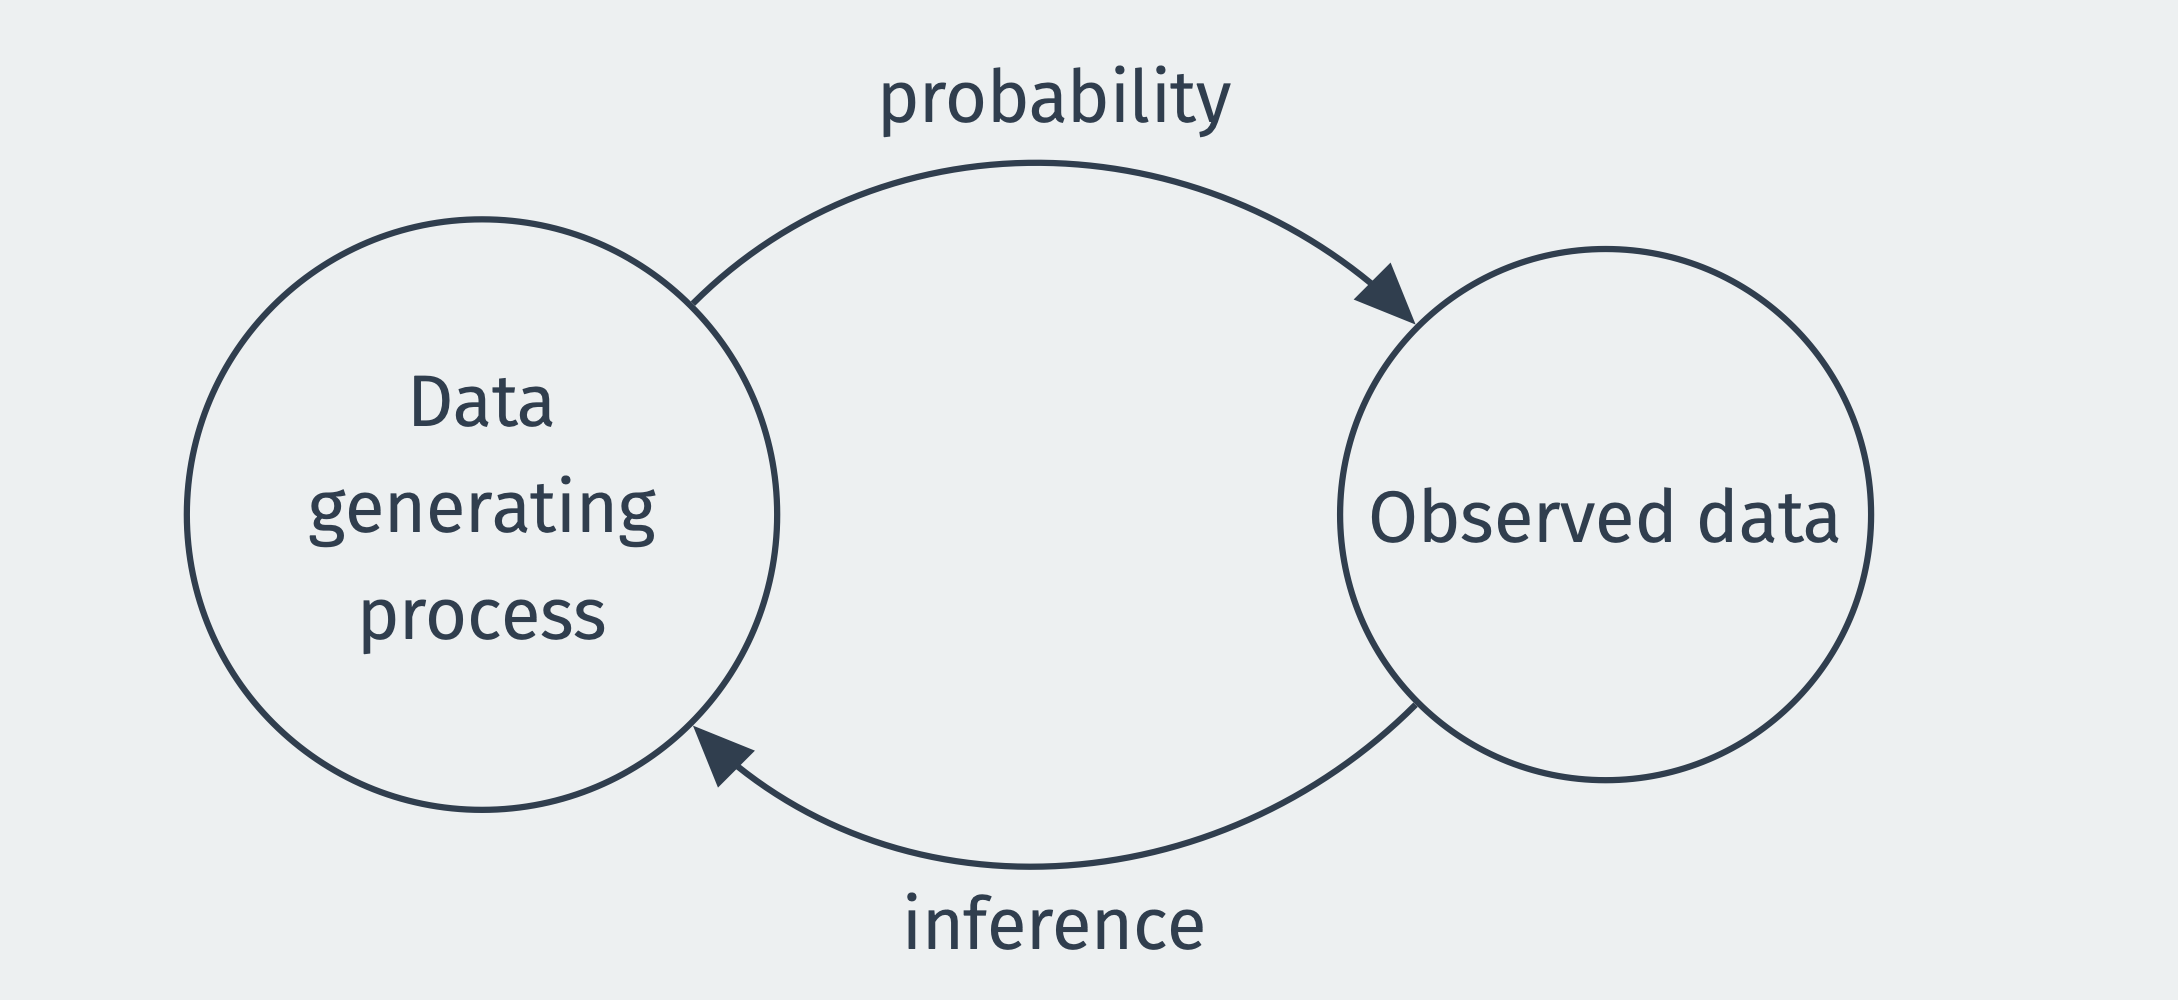
\includegraphics{assets/img/two-direction.png}

An estimator is a rule for converting our data into a best guess about
some unknown quantity, such as the percent of balls in the urn, or, to
use our example from the introduction, the fraction of the public
supporting increasing legal immigration limits. For example, an
estimator could be a rule that the proportion of red balls that you draw
from the urn is a good guess for the proportion of red balls that you
would find if you looked inside the urn.

We prefer to use \textbf{good} estimators rather than \textbf{bad}
estimators. But what makes an estimator good or bad? In our red ball
example, an estimator that always returns the value 3 is probably bad.
Still, it will be helpful for us to formally define and explore
properties of estimators that will allow us to compare them and choose
the good over the bad. We begin with an example that highlights two
estimators that at first glance may seem similar.

\begin{example}[Randomized control
trial]\protect\hypertarget{exm-rct}{}\label{exm-rct}

Suppose we are conducting a randomized experiment on framing effects.
All respondents receive factual information about current immigration
levels. Those in the treatment group (\(D_i = 1\)) receive additional
information about the positive benefits of immigration, while those in
the control group (\(D_i = 0\)) receive no additional framing. The
outcome is a binary outcome, whether the respondent supports increasing
legal immigration limits (\(Y_i = 1\)) or not (\(Y_i = 0\)). The
observed data consists of \(n\) pairs of random variables, the outcome,
and the treatment assignment: \(\{(Y_1, D_1), \ldots, (Y_n, D_n)\}\).

Define the two sample means/proportions in each group as \[
\Ybar_1 = \frac{1}{n_1} \sum_{i: D_i = 1} Y_i, \qquad\qquad \Ybar_0 = \frac{1}{n_0} \sum_{i: D_i = 0} Y_i,
\] where \(n_1 = \sum_{i=1}^n D_i\) is the number of treated units and
\(n_0 = n - n_1\) is the number of control units.

A standard estimator for the treatment effect in a study such as this
would be the difference in means, \(\Ybar_1 - \Ybar_0\). But this is
only one of many possible estimators. We could also estimate the effect
by taking this difference in means separately by party identification
and then averaging those party-specific effects by the size of those
groups. This estimator is commonly called a \textbf{poststratification}
estimator. Which of these two estimators we should prefer is at first
glance unclear.

\end{example}

We now turn to the same key questions that we used to motivate
design-based inference, but adapt these to consider model-based
inference.

\section{Question 1: Population}\label{question-1-population-1}

The main advantage and disadvantage of relying on models is that they
are abstract and theoretical, which means the connection between a model
and the population it helps explain is less direct than with the
design-based framework. Nevertheless, we need to clearly articulate our
population of study -- that is, who or what we want to learn about --
since it is crucial for evaluating the types of modeling assumptions
that will be sustainable.

As in the design-based setting, there is often a clear and distinct
population such as ``all registered voters'' or ``all Boston
residents.'' In other cases, the population may be more abstract. For
example, a large multi-field literature has studied how the size of
minority populations affects the views of the local majority population.
Researchers in this space may be interested in making claims beyond the
particular geographic region or minority/majority group, instead
implicitly or explicitly considering a ``superpopulation'' of such cases
that their model might explain. While there is nothing theoretically
wrong with this approach, these ideas are often neglected in practice
and the ``scope conditions'' of a particular model go unarticulated. The
best quantitative work will be clear about what units or processes it is
trying to learn about so that readers can evaluate how well the modeling
assumptions fit that task.

\section{Question 2: Statistical
model}\label{question-2-statistical-model}

Let's begin by building a bare-bones probability model for how our data
came to be. As an example, suppose we have a data set with a series of
numbers representing the ages, political party affiliations, and policy
opinions of 1000 survey respondents. But we know that row 58 of our data
could have produced a different set of numbers if another respondent had
been selected as row 58 or if the original respondent gave a different
opinion about immigration because they happened to see an immigration
news story just before responding. To reason about this type of
uncertainty precisely, we write \(X_i\) as the random variable
representing the value that row \(i\) of some variable will take, before
we see the data. The distribution of this random variable would tell us
what types of data we should expect to see.

Why represent the data with random variables when we already know the
value of the data itself? Why pretend we haven't seen the data? The
study of estimation from a frequentist perspective (which is the
perspective of this book) focuses on the properties of estimators across
\textbf{repeated samples}. In the example of the policy survey, this is
akin to drawing a 1000 person sample repeatedly, each time including
possibly different respondents in the sample. The random variable
\(X_i\) represents our uncertainty about what value, say, age will take
for respondent \(i\) in any of these samples, and the set
\(\{X_{1}, \ldots, X_{n}\}\) represents our uncertainty about the entire
column of ages for all \(n\) respondents. At the most general, the
model-based approach says that these \(n\) random variables follow some
joint distribution, \(F_{X_{1},\ldots,X_{n}}\), \[
\{X_{1}, \ldots, X_{n}\} \sim F_{X_{1},\ldots,X_{n}}
\] The joint distribution \(F\) here represents the probability model
for the data. We have made no assumptions about it so far, so it could
be any joint probability distribution over \(n\) random variables. Note
that this level of generality is difficult to work with in practice
because there is essentially one draw from this joint distribution (the
\(n\) measurements in the data). The core question of modeling is about
what restrictions a researcher puts on this joint distribution to make
learning about it more tractable.

We focus on a relatively simple setting where we assume the data
\(\{X_1, \ldots, X_n\}\) are \textbf{independent and identically
distributed} (iid) draws from a distribution with cumulative
distribution function (cdf) \(F\). They are independent in that
information about any subset of random variable is not informative about
any other subset of random variables, or, more formally, \[
F_{X_{1},\ldots,X_{n}}(x_{1}, \ldots, x_{n}) = F_{X_{1}}(x_{1})\cdots F_{X_{n}}(x_{n}) = \prod_{i=1}^n F(x_i)
\] where \(F_{X_{1},\ldots,X_{n}}(x_{1}, \ldots, x_{n})\) is the joint
cdf of the random variable and \(F_{X_{j}}(x_{j})\) is the marginal cdf
of the \(j\)th random variable. They are ``identically distributed'' in
the sense that each of the random variables \(X_i\) have the same
marginal distribution, \(F\).

Note that we are being purposely vague about this cdf---it simply
represents the unknown distribution of the data, otherwise known as the
\textbf{data generating process} (DGP). Sometimes \(F\) is also referred
to as the \textbf{population distribution} or even just
\textbf{population}, which has its roots in viewing the data as a random
sample from some larger population.{[}\^{}model{]} As a shorthand, we
often say that the collection of random variables
\(\{X_1, \ldots, X_n\}\) is a \textbf{random sample} from population
\(F\) if \(\{X_1, \ldots, X_n\}\) is iid with distribution \(F\). The
\textbf{sample size} \(n\) is the number of units in the sample.

\begin{tcolorbox}[enhanced jigsaw, toptitle=1mm, bottomrule=.15mm, leftrule=.75mm, rightrule=.15mm, breakable, colframe=quarto-callout-note-color-frame, title=\textcolor{quarto-callout-note-color}{\faInfo}\hspace{0.5em}{Note}, colbacktitle=quarto-callout-note-color!10!white, titlerule=0mm, coltitle=black, left=2mm, colback=white, bottomtitle=1mm, opacitybacktitle=0.6, opacityback=0, toprule=.15mm, arc=.35mm]

You might wonder why we reference the distribution of \(X_i\) with the
cdf, \(F\). Mathematical statistics tends to do this to avoid having to
deal with discrete and continuous random variables separately. Every
random variable -- whether discrete or continuous -- has a cdf, and the
cdf contains all information about the distribution of a random
variable.

\end{tcolorbox}

Two metaphors help build intuition behind viewing the data as an iid
draw from \(F\):

\begin{enumerate}
\def\labelenumi{\arabic{enumi}.}
\tightlist
\item
  \textbf{Random sampling}. Suppose we have a population of size \(N\)
  that is much larger than our sample size \(n\), and we take a random
  sample of size \(n\) from this population with replacement. The
  distribution of the data in the random sample will be iid draws from
  the population distribution of the variables we are sampling. For
  example, suppose the population proportion of Democratic party
  identifiers among U.S. citizens is 0.33. If we randomly sample
  \(n = 100\) U.S. citizens, each data point \(X_i\) will be distributed
  Bernoulli with a probability of success (i.e., Democratic Party
  identifier) of 0.33.
\end{enumerate}

Note that the last chapter explored simple random samples \emph{without
replacement}, which is a more common type of sampling -- since generally
people are selected into a survey once and they do not go back into the
pool of potential survey takers. Sampling without replacement creates
dependence across units, which would violate the iid assumption.
However, if the population size \(N\) is very large relative to the
sample size \(n\), this dependence will be very small, and the iid
assumption will be relatively innocuous.

\begin{enumerate}
\def\labelenumi{\arabic{enumi}.}
\setcounter{enumi}{1}
\tightlist
\item
  \textbf{Groundhog Day}. Random sampling does not always make sense as
  a justification for iid data, especially when the units are not
  samples at all but rather countries, states, or subnational units. (In
  these cases, the population can be the same as the sample -- for
  example, using all 50 states to draw conclusions on the efficacy of
  state policy.) In this case, we have to appeal to a thought experiment
  where \(F\) represents the fundamental uncertainty in the
  data-generating process. The metaphor here is that if we could re-run
  history many times, such as what happens to the protagonist played by
  Bill Murray in the 1993 American comedy movie \emph{Groundhog Day}
  when he is magically forced to relive February 2 over and over again.
  Under this fiction, data and outcomes would change slightly due to the
  inherently stochastic nature of the world. In the movie, for example,
  Murray's character starts off the same day in exactly the same way,
  but he begins to change his actions and the outcomes at the end of
  each day change in subtle ways. The iid assumption, then, is that each
  of the units in our data has the same DGP producing this data or the
  same distribution of outcomes under the \emph{Groundhog Day} scenario.
  The set of all these infinite possible draws from the DGP is sometimes
  referred to as the \textbf{superpopulation}.
\end{enumerate}

Note that there are other situations where the iid assumption is not
appropriate, which we discuss in later chapters. But much of the
innovation and growth in statistics over the last 50 years has been in
figuring out how to make statistical inferences when iid does not hold.
The solutions are often specific to the type of iid violation (e.g.,
spatial, time-series, network, clustered). As a rule of thumb, however,
if the iid assumption may not be valid, any uncertainty statements will
likely be overconfident. For example, confidence intervals, which we
will cover in later chapters, are too small.

Finally, we introduced the data as a scalar random variable, but often
our data has multiple variables. In that case, we easily modify \(X_i\)
to be a random vector (that is, a vector of random variables) and then
\(F\) becomes the joint distribution of that random vector. Nothing
substantive changes about the above discussion.

\begin{tcolorbox}[enhanced jigsaw, toptitle=1mm, bottomrule=.15mm, leftrule=.75mm, rightrule=.15mm, breakable, colframe=quarto-callout-warning-color-frame, title=\textcolor{quarto-callout-warning-color}{\faExclamationTriangle}\hspace{0.5em}{Warning}, colbacktitle=quarto-callout-warning-color!10!white, titlerule=0mm, coltitle=black, left=2mm, colback=white, bottomtitle=1mm, opacitybacktitle=0.6, opacityback=0, toprule=.15mm, arc=.35mm]

Survey sampling is one of the most popular ways of obtaining samples
from a population, but modern sampling practices rarely produce a
``clean'' set of \(n\) iid responses. There are several reasons for
this:

\begin{itemize}
\item
  Modern random sampling techniques generally do not select every unit
  with the same probability. We might \emph{oversample} certain groups
  for which we want more precise estimates, leading those groups to have
  a higher likelihood of being in the sample.
\item
  Response rates to surveys have been in steep decline and can often dip
  below 10\%. Such non-random selection into the observed sample might
  lead to problems.
\item
  Internet polling is less costly than other forms of polling, but
  obtaining a list of population email addresses (or other digital
  contact information) to randomly sample is basically impossible. Large
  survey firms instead recruit large groups of panelists with known
  demographic information from which they can randomly sample in a way
  that matches population demographic information. Because the initial
  opt-in panel is not randomly sampled from the population, this
  procedure does not produce a true ``random sample,'' but, under
  certain assumptions, we can treat it like it is.
\end{itemize}

As discussed in the last chapter, there are ways to handle all of these
issues (mostly through the use of survey weights), but it is important
to realize that using a modern survey ``as if'' it was a simple random
sample might lead to poor performance and incorrect inferences.

\end{tcolorbox}

\section{Question 3: Quantities of
interest}\label{question-3-quantities-of-interest}

In model-based inference, our goal is to learn about the data-generating
process. Each data point \(X_i\) represents a draw from a distribution,
captured by the cdf \(F\), and we would like to know more about this
distribution. We might be interested in estimating the cdf at a general
level or only some feature of the distribution, like a mean or
conditional expectation function. We call these numerical features the
\textbf{quantities of interest}. (Similarly, in the design-based
inference framework we discussed in the previous chapter, the quantity
of interest was a numerical summary of the finite population.)

The following are examples of frequently used quantities of interest:

\begin{example}[Population
mean]\protect\hypertarget{exm-prop}{}\label{exm-prop}

We may be interested in where the typical member of a population falls
on some questions. Suppose we wanted to know the proportion of US
citizens who support increasing legal immigration For citizen \(i\),
denote support as \(Y_i = 1\). Our quantity of interest is then the mean
of this random variable, \(\mu = \E[Y_i] = \P(Y_{i} = 1)\). This is the
same as the probability of randomly drawing someone from the population
who supports increasing legal immigration.

\end{example}

\begin{example}[Population
variance]\protect\hypertarget{exm-var}{}\label{exm-var}

We may also be interested in variation in the population. For example,
feeling thermometer scores are a common way to assess how survey
respondents feel about a particular person or group. These ask each
respondent to say how warmly he or she feels toward a group on a scale
from 0 (cool) to 100 (warm), which we will denote \(Y_i\). We might be
interested in how polarized views are toward a group in the population,
and one measure of polarization could be the variance, or spread, of the
distribution of \(Y_i\) around the mean. In this case,
\(\sigma^2 = \V[Y_i] = \E[(Y_i - \E[Y_i])^2]\) would be our quantity of
interest.

\end{example}

\begin{example}[RCT
continued]\protect\hypertarget{exm-rct-ii}{}\label{exm-rct-ii}

Example~\ref{exm-rct} discussed a typical estimator for an experimental
study with a binary treatment. The goal of that experiment is to learn
about the difference between two conditional probabilities (or
expectations): 1) the average support for increasing legal immigration
in the treatment group, \(\mu_1 = \E[Y_i \mid D_i = 1]\), and 2) the
same average in the control group, \(\mu_0 = \E[Y_i \mid D_i = 0]\).
This difference, \(\mu_1 - \mu_0\), is a function of unknown features of
these two conditional distributions.

\end{example}

Each of these is a function of the (possibly joint) distribution of the
data, \(F\). In each of these, we are not necessarily interested in the
entire distribution, just summaries of it (central tendency, spread). Of
course, there are situations where we are also interested in the
complete distribution. To speak about estimation in general, we will let
\(\theta\) represent some generic quantity of interest. \textbf{Point
estimation} describes how we obtain a single ``best guess'' about
\(\theta\).

\begin{tcolorbox}[enhanced jigsaw, toptitle=1mm, bottomrule=.15mm, leftrule=.75mm, rightrule=.15mm, breakable, colframe=quarto-callout-note-color-frame, title=\textcolor{quarto-callout-note-color}{\faInfo}\hspace{0.5em}{Note}, colbacktitle=quarto-callout-note-color!10!white, titlerule=0mm, coltitle=black, left=2mm, colback=white, bottomtitle=1mm, opacitybacktitle=0.6, opacityback=0, toprule=.15mm, arc=.35mm]

Some refer to quantities of interest as \textbf{parameters} or
\textbf{estimands} (that is, the target of estimation).

\end{tcolorbox}

\section{Question 4: Estimator}\label{question-4-estimator-1}

Having a target in mind, we can estimate it with our data. To do so, we
first need a rule or algorithm or function that takes as inputs the data
and returns a best guess about the quantity of interest. One of the most
popular and useful algorithm would be to sum all the data points and
divide by the number of points: \[
\frac{X_1 + X_2 + \cdots + X_n}{n}.
\] This, the much-celebrated sample mean, provides a rule for how
produce a single-number summary of the data. To go one pedantic step
further and define it as a function of the data more explicitly: \[
\textsf{mean}(X_1, X_2, \ldots, X_n) = \frac{X_1 + X_2 + \cdots + X_n}{n}.
\] We can use this model to provide a definition for an arbitrary
estimator for an arbitrary quantity of interest.

\begin{definition}[]\protect\hypertarget{def-estimator}{}\label{def-estimator}

An \textbf{estimator} \(\widehat{\theta}_n = \theta(X_1, \ldots, X_n)\)
for some parameter \(\theta\), is a function of the data intended as a
guess about \(\theta\).

\end{definition}

\begin{tcolorbox}[enhanced jigsaw, toptitle=1mm, bottomrule=.15mm, leftrule=.75mm, rightrule=.15mm, breakable, colframe=quarto-callout-note-color-frame, title=\textcolor{quarto-callout-note-color}{\faInfo}\hspace{0.5em}{Note}, colbacktitle=quarto-callout-note-color!10!white, titlerule=0mm, coltitle=black, left=2mm, colback=white, bottomtitle=1mm, opacitybacktitle=0.6, opacityback=0, toprule=.15mm, arc=.35mm]

It is widespread, though not universal, to use the ``hat'' notation to
define an estimator and its estimand. For example, \(\widehat{\theta}\)
(or ``theta hat'') indicates that this estimator is targeting the
parameter \(\theta\).

\end{tcolorbox}

\begin{example}[Estimators for the population
mean]\protect\hypertarget{exm-mean-est}{}\label{exm-mean-est}

Suppose our goal is to estimate the population mean of \(F\), which we
will represent as \(\mu = \E[X_i]\). We could choose from several
estimators, all with different properties. \[
\widehat{\theta}_{n,1} = \frac{1}{n} \sum_{i=1}^n X_i, \quad \widehat{\theta}_{n,2} = X_1, \quad \widehat{\theta}_{n,3} = \text{max}(X_1,\ldots,X_n), \quad \widehat{\theta}_{n,4} = 3
\] The first is just the sample mean, which is an intuitive and natural
estimator for the population mean. The second just uses the first
observation. While this seems silly, this is a valid statistic since it
is a function of the data! The third takes the maximum value in the
sample, and the fourth always returns three, regardless of the data.
These are also valid statistics.

\end{example}

When we view the data \(\{X_{1}, \ldots, X_{n}\}\) as a collection of
random variables, then any function of them is also a random variable.
Thus, we can view \(\widehat{\theta}_n\) as a random variable that has a
distribution induced by the randomness of the sample. Drawing two
different samples of respondents will lead to two different estimates.
For example, here we illustrate two samples of size \(n =5\) from the
population distribution of a binary variable:

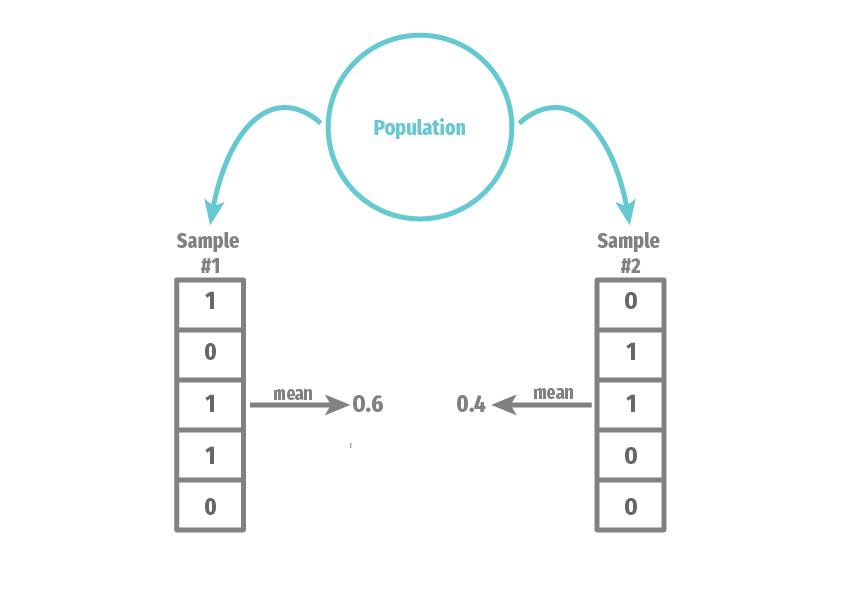
\includegraphics{assets/img/sampling-distribution.png}

We can see that the mean of the variable depends on what exact values
end up in our sample. We refer to the distribution of
\(\widehat{\theta}_n\) across repeated samples as its \textbf{sampling
distribution}. The sampling distribution of an estimator will be the
basis for all of the formal statistical properties of an estimator.

\begin{tcolorbox}[enhanced jigsaw, toptitle=1mm, bottomrule=.15mm, leftrule=.75mm, rightrule=.15mm, breakable, colframe=quarto-callout-warning-color-frame, title=\textcolor{quarto-callout-warning-color}{\faExclamationTriangle}\hspace{0.5em}{Warning}, colbacktitle=quarto-callout-warning-color!10!white, titlerule=0mm, coltitle=black, left=2mm, colback=white, bottomtitle=1mm, opacitybacktitle=0.6, opacityback=0, toprule=.15mm, arc=.35mm]

One important distinction of jargon is between an estimator and an
estimate. The estimator is a function of the data, whereas the
\textbf{estimate} is the \emph{realized value} of the estimator once we
see the data (that is, the data are realized). The estimator is a random
variable that has uncertainty over what value it will take, and we
represent the estimator as a function of random variables,
\(\widehat{\theta}_n = \theta(X_1, \ldots, X_n)\). An estimate is a
single number, such as 0.38, that we calculated in R with our data (our
draw from \(F\)). Formally, the estimate is \(\theta(x_1, \ldots, x_n)\)
when the data is \(\{X_1, \ldots, X_n\} = \{x_1, \ldots, x_n\}\),
whereas we represent the estimator as a function of random variables,
\(\widehat{\theta}_n = \theta(X_1, \ldots, X_n)\).

\end{tcolorbox}

\section{How to find estimators}\label{how-to-find-estimators}

Where do estimators come from? That may seem like a question reserved
for statisticians or methodologists or others responsible for
``developing new methods.'' But knowing how estimators are derived is
valuable even if we never plan to do it ourselves. Knowing where an
estimator comes from provides strong insights into its strengths and
weaknesses. We will briefly introduce estimators based on parametric
models, before turning to the main focus of this book, plug-in
estimators.

\subsection{Parametric models and maximum
likelihood}\label{parametric-models-and-maximum-likelihood}

The first method for generating estimators relies on \textbf{parametric
models}, in which the researcher specifies the exact distribution (up to
some unknown parameters) of the DGP. Let \(\theta\) be the parameters of
this distribution, where \(\{X_1, \ldots, X_n\}\) be iid draws from
\(F_{\theta}\). We should also formally state the set of possible values
the parameters can take, which we call the \textbf{parameter space},
denoted by \(\Theta\). Because we assume we know the distribution of the
data, we can write the probability density function, or pdf, as
\(f(X_i \mid \theta)\) and define the likelihood function as the product
of these pdfs over the units as a function of the parameters: \[
L(\theta) = \prod_{i=1}^n f(X_i \mid \theta).
\] We can then define the \textbf{maximum likelihood} estimator (MLE)
for \(\theta\) as the values of the parameter that, well, maximize the
likelihood: \[
\widehat{\theta}_{mle} = \argmax_{\theta \in \Theta} \; L(\theta)
\] Sometimes we can use calculus to derive a closed-form expression for
the MLE. At other times we use iterative techniques that search the
parameter space for the maximum.

Maximum likelihood estimators have nice properties, especially in large
samples. Unfortunately, they also require the correct knowledge of the
parametric model, which is often difficult to justify. Do we really know
if we should model a given event count variable as Poisson or Negative
Binomial? The attractive properties of MLE are only as good as the
ability to specify the parametric model.

\begin{tcolorbox}[enhanced jigsaw, toptitle=1mm, bottomrule=.15mm, leftrule=.75mm, rightrule=.15mm, breakable, colframe=quarto-callout-note-color-frame, title=\textcolor{quarto-callout-note-color}{\faInfo}\hspace{0.5em}{No free lunch}, colbacktitle=quarto-callout-note-color!10!white, titlerule=0mm, coltitle=black, left=2mm, colback=white, bottomtitle=1mm, opacitybacktitle=0.6, opacityback=0, toprule=.15mm, arc=.35mm]

Building up intuition about the \textbf{assumptions-precision tradeoff}
is essential. Researchers can usually get more precise estimates if they
make stronger and potentially more fragile assumptions. Conversely, they
will almost always get less accurate estimates when weakening the
assumptions.

\end{tcolorbox}

\subsection{Plug-in estimators}\label{plug-in-estimators}

The second broad class of estimators is \textbf{semiparametric} in that
we specify some finite-dimensional parameters of the DGP but leave the
rest of the distribution unspecified. For example, we might define a
population mean, \(\mu = \E[X_i]\) and a population variance,
\(\sigma^2 = \V[X_i]\) but leave the shape of the distribution
unrestricted. This ensures that our estimators will be less dependent on
correctly specifying distributions about which we have little intuition
or knowledge.

The primary method for constructing estimators in this setting is to use
the \textbf{plug-in estimator}, or the estimator that replaces any
population mean with a sample mean. Obviously, in the case of estimating
the population mean, \(\mu\), we will use the \textbf{sample mean} as
the estimate: \[
\Xbar_n = \frac{1}{n} \sum_{i=1}^n X_i \quad \text{estimates} \quad \E[X_i] = \int_{\mathcal{X}} x f(x)dx
\] In plain language, we are replacing the unknown population
distribution \(f(x)\) in the population mean with a discrete uniform
distribution over our data points, with \(1/n\) probability assigned to
each unit. Why do this? It encodes that, if we have a random sample, our
best guess about the population distribution of \(X_i\) is the sample
distribution in our observed data. If this intuition fails, you can hold
onto an analog principle: sample means of random variables are natural
estimators of population means.

What about estimating something more complicated, like the expected
value of a function of the data, \(\theta = \E[r(X_i)]\)? The key is to
see that \(r(X_i)\) is also a random variable. Let this random variable
be \(Y_i = r(X_i)\). Now we can see that \(\theta\) is just the
population expectation of this random variable. Using the plug-in
estimator gives us: \[
\widehat{\theta} = \frac{1}{n} \sum_{i=1}^n Y_i = \frac{1}{n} \sum_{i=1}^n r(X_i). 
\]

These facts enable us to describe a more general plug-in estimator. To
estimate some quantity of interest that is a function of population
means, we can generate a plug-in estimator by replacing any population
mean with a sample mean. Formally, let
\(\alpha = g\left(\E[r(X_i)]\right)\) be a parameter that is defined as
a function of the population mean of a (possibly vector-valued) function
of the data. We can then estimate this parameter by plugging in the
sample mean for the population mean to get the \textbf{plug-in
estimator}, \[
\widehat{\alpha} = g\left( \frac{1}{n} \sum_{i=1}^n r(X_i) \right) \quad \text{estimates} \quad \alpha = g\left(\E[r(X_i)]\right)
\] This approach to plug-in estimation with sample means is very general
and will allow us to derive estimators in various settings.

\begin{example}[Estimating population
variance]\protect\hypertarget{exm-var-est}{}\label{exm-var-est}

The population variance of a random variable is
\(\sigma^2 = \E[(X_i - \E[X_i])^2]\). To derive a plug-in estimator for
this quantity, we replace the inner \(\E[X_i]\) with \(\Xbar_n\) and the
outer expectation with another sample mean: \[
\widehat{\sigma}^2 = \frac{1}{n} \sum_{i=1}^n (X_i - \Xbar_n)^2.
\] This plug-in estimator differs from the standard sample variance,
which divides by \(n - 1\) rather than \(n\). This minor difference does
not matter in moderate to large samples.

\end{example}

\begin{example}[Estimating population
covariance]\protect\hypertarget{exm-cov-est}{}\label{exm-cov-est}

Suppose we have two variables, \((X_i, Y_i)\). A natural quantity of
interest here is the population covariance between these variables, \[
\sigma_{xy} = \text{Cov}[X_i,Y_i] = \E[(X_i - \E[X_i])(Y_i-\E[Y_i])],
\] which has the plug-in estimator, \[
\widehat{\sigma}_{xy} = \frac{1}{n} \sum_{i=1}^n (X_i - \Xbar_n)(Y_i - \Ybar_n).
\]

\end{example}

\begin{tcolorbox}[enhanced jigsaw, toptitle=1mm, bottomrule=.15mm, leftrule=.75mm, rightrule=.15mm, breakable, colframe=quarto-callout-note-color-frame, title=\textcolor{quarto-callout-note-color}{\faInfo}\hspace{0.5em}{Notation alert}, colbacktitle=quarto-callout-note-color!10!white, titlerule=0mm, coltitle=black, left=2mm, colback=white, bottomtitle=1mm, opacitybacktitle=0.6, opacityback=0, toprule=.15mm, arc=.35mm]

Given the connection between the population mean and the sample mean,
you may see the \(\E_n[\cdot]\) operator used as a shorthand for the
sample average: \[
\E_n[r(X_i)] \equiv \frac{1}{n} \sum_{i=1}^n r(X_i).
\]

\end{tcolorbox}

Finally, plug-in estimation goes beyond just replacing population means
with sample means. We can derive estimators of the population quantiles
like the median with sample versions of those quantities. These
approaches are unified in replacing the unknown population cdf, \(F\),
with the empirical cdf, \[
\widehat{F}_n(x) = \frac{\sum_{i=1}^n \mathbb{I}(X_i \leq x)}{n},
\] where \(\mathbb{I}(A)\) is an \emph{indicator function} that takes
the value 1 if the event \(A\) occurs and 0 otherwise. For a more
complete and technical treatment of these ideas, see Wasserman (2004)
Chapter 7.

\section{The three distributions: population, empirical, and
sampling}\label{the-three-distributions-population-empirical-and-sampling}

Once we start to wade into estimation, there are several distributions
to keep track of, and things can quickly become confusing. Three
specific distributions are all related and easy to confuse, but keeping
them distinct is crucial.

The \textbf{population distribution} is the distribution of the random
variable, \(X_i\), which we have labeled \(F\) and is our target of
inference. The \textbf{empirical distribution} is the distribution of
the actual realizations of the random variables in our samples,
\(X_1, \ldots, X_n\) (that is, the values that we eventually observe in
our data frame). Because this is a random sample from the population
distribution and can serve as an estimator of \(F\), we sometimes call
this \(\widehat{F}_n\).

Separately from both is the \textbf{sampling distribution of an
estimator}, which is the probability distribution of
\(\widehat{\theta}_n\). This represents the uncertainty around our
estimate before we see the data. Remember that our estimator is itself a
random variable because it is a function of random variables: the data
itself. That is, we defined the estimator as
\(\widehat{\theta}_n = \theta(X_1, \ldots, X_n)\).

\begin{example}[Likert
responses]\protect\hypertarget{exm-three-dist}{}\label{exm-three-dist}

Suppose \(X_i\) is the answer to the question ``How much do you agree
with the following statement: Immigrants are a net positive for the
United States,'' where \(X_i = 0\) is ``strongly disagree,'' \(X_i = 1\)
is ``disagree,'' \(X_i = 2\) is ``neither agree nor disagree,''
\(X_i = 3\) is ``agree,'' and \(X_i = 4\) is ``strongly agree.''

The population distribution describes the probability of randomly
selecting a person with each one of these values, \(\P(X_i = x)\). The
empirical distribution would be the fraction of our observed data taking
each value. And the sampling distribution of the sample mean,
\(\Xbar_n\), would be the distribution of the sample mean recalculated
across repeated samples from the population.

Suppose the population distribution of \(X_i\) followed a binomial
distribution with five trials and probability of success in each trial
of \(p = 0.4\). We could generate one sample with \(n = 10\) and thus
one empirical distribution using \texttt{rbinom()}:

\begin{Shaded}
\begin{Highlighting}[]
\NormalTok{my\_samp }\OtherTok{\textless{}{-}} \FunctionTok{rbinom}\NormalTok{(}\AttributeTok{n =} \DecValTok{10}\NormalTok{, }\AttributeTok{size =} \DecValTok{4}\NormalTok{, }\AttributeTok{prob =} \FloatTok{0.4}\NormalTok{)}
\NormalTok{my\_samp}
\end{Highlighting}
\end{Shaded}

\begin{verbatim}
 [1] 1 2 1 3 3 0 2 3 2 1
\end{verbatim}

\begin{Shaded}
\begin{Highlighting}[]
\FunctionTok{table}\NormalTok{(my\_samp)}
\end{Highlighting}
\end{Shaded}

\begin{verbatim}
my_samp
0 1 2 3 
1 3 3 3 
\end{verbatim}

We obtain one draw from the sampling distribution of \(\Xbar_n\) by
taking the mean of this sample:

\begin{Shaded}
\begin{Highlighting}[]
\FunctionTok{mean}\NormalTok{(my\_samp)}
\end{Highlighting}
\end{Shaded}

\begin{verbatim}
[1] 1.8
\end{verbatim}

If we had a different sample,however, we would obtain a different
empirical distribution and thus get a different estimate of the sample
mean:

\begin{Shaded}
\begin{Highlighting}[]
\NormalTok{my\_samp2 }\OtherTok{\textless{}{-}} \FunctionTok{rbinom}\NormalTok{(}\AttributeTok{n =} \DecValTok{10}\NormalTok{, }\AttributeTok{size =} \DecValTok{4}\NormalTok{, }\AttributeTok{prob =} \FloatTok{0.4}\NormalTok{)}
\FunctionTok{mean}\NormalTok{(my\_samp2) }
\end{Highlighting}
\end{Shaded}

\begin{verbatim}
[1] 1.6
\end{verbatim}

The sampling distribution is the distribution of these sample means
across repeated sampling.

\end{example}

\section{Finite-sample properties of
estimators}\label{finite-sample-properties-of-estimators}

As discussed in our introduction to estimators, their usefulness depends
on how well they help us learn about the quantity of interest. If we get
an estimate \(\widehat{\theta} = 1.6\), we would like to know that this
is ``close'' to the true parameter \(\theta\). The sampling distribution
is key to answering these questions. Intuitively, we would like the
sampling distribution of \(\widehat{\theta}_n\) to be as tightly
clustered around the true \(\theta\) as possible. Here, though, we run
into a problem: the sampling distribution depends on the population
distribution since it is about repeated samples of the data from that
distribution filtered through the function \(\theta()\). Since \(F\) is
unknown, this implies that the sampling distribution will also usually
be unknown.

Even though we cannot precisely pin down the entire sampling
distribution, we can use assumptions to derive specific properties of
the sampling distribution that are useful in comparing estimators. Note
that the properties here will be very similar to the

\subsection{Bias}\label{bias}

The first property of the sampling distribution concerns its central
tendency. In particular, we define the \textbf{bias} (or
\textbf{estimation bias}) of estimator \(\widehat{\theta}\) for
parameter \(\theta\) as \[
\text{bias}[\widehat{\theta}] = \E[\widehat{\theta}] - \theta,
\] which is the difference between the mean of the estimator (across
repeated samples) and the true parameter. All else equal, we would like
the estimation bias to be as small as possible. The smallest possible
bias, obviously, is 0, and we define an \textbf{unbiased estimator} as
one with \(\text{bias}[\widehat{\theta}] = 0\) or equivalently,
\(\E[\widehat{\theta}] = \theta\).

However, all else is not always equal, and unbiasedness is not a
property to which we should become overly attached. Many biased
estimators have other attractive properties, and many popular modern
estimators are biased.

\begin{example}[Unbiasedness of the sample
mean]\protect\hypertarget{exm-mean-unbiased}{}\label{exm-mean-unbiased}

The sample mean is unbiased for the population mean when the data is iid
and \(\E|X| < \infty\). In particular, we apply the rules of
expectations: \[\begin{aligned}
\E\left[ \Xbar_n \right] &= \E\left[\frac{1}{n} \sum_{i=1}^n X_i\right] & (\text{definition of } \Xbar_n) \\
&= \frac{1}{n} \sum_{i=1}^n \E[X_i] & (\text{linearity of } \E)\\
&= \frac{1}{n} \sum_{i=1}^n \mu & (X_i \text{ identically distributed})\\
&= \mu.
\end{aligned}\] Notice that we only used the ``identically distributed''
part of iid. Independence is not needed.

\end{example}

\begin{tcolorbox}[enhanced jigsaw, toptitle=1mm, bottomrule=.15mm, leftrule=.75mm, rightrule=.15mm, breakable, colframe=quarto-callout-warning-color-frame, title=\textcolor{quarto-callout-warning-color}{\faExclamationTriangle}\hspace{0.5em}{Warning}, colbacktitle=quarto-callout-warning-color!10!white, titlerule=0mm, coltitle=black, left=2mm, colback=white, bottomtitle=1mm, opacitybacktitle=0.6, opacityback=0, toprule=.15mm, arc=.35mm]

Properties like unbiasedness might only hold for a subset of DGPs. For
example, we just showed that the sample mean is unbiased but only when
the population mean is finite. There are probability distributions like
the Cauchy that are not finite and where the expected value diverges.
Thus, here we are dealing with a restricted class of DGPs that rules out
such distributions. This is sometimes formalized by defining a class
\(\mathcal{F}\) of distributions; unbiasedness might hold in that class
if it is unbiased for all \(F \in \mathcal{F}\).

\end{tcolorbox}

\section{Question 5: Uncertainty}\label{question-5-uncertainty-1}

The spread of the sampling distribution is also important. We define the
\textbf{sampling variance} as the variance of an estimator's sampling
distribution, \(\V[\widehat{\theta}]\), which measures how spread out
the estimator is around its mean. For an unbiased estimator, lower
sampling variance implies the distribution of \(\widehat{\theta}\) is
more concentrated around the true value of the parameter.

\begin{example}[Sampling variance of the sample
mean]\protect\hypertarget{exm-mean-var}{}\label{exm-mean-var}

We can prove that the sampling variance of the sample mean of iid data
for all \(F\) such that \(\V[X_i]\) is finite (more precisely,
\(\E[X_i^2] < \infty\))

\[\begin{aligned}
  \V\left[ \Xbar_n \right] &= \V\left[ \frac{1}{n} \sum_{i=1}^n X_i \right] & (\text{definition of } \Xbar_n) \\
                           &= \frac{1}{n^2} \V\left[ \sum_{i=1}^n X_i \right] & (\text{property of } \V) \\
                           &= \frac{1}{n^2} \sum_{i=1}^n \V[X_i] & (\text{independence}) \\
                           &= \frac{1}{n^2} \sum_{i=1}^n \sigma^2 & (X_i \text{ identically distributed}) \\
                           &= \frac{\sigma^2}{n}
\end{aligned}\]

\end{example}

As we discussed before, an alternative measure of spread for any
distribution is the standard deviation, which is on the same scale as
the original random variable. The standard deviation of the sampling
distribution of \(\widehat{\theta}\) is known as the \textbf{standard
error} of \(\widehat{\theta}\):
\(\se(\widehat{\theta}) = \sqrt{\V[\widehat{\theta}]}\).

Given the above derivation, the standard error of the sample mean under
iid sampling is \(\sigma / \sqrt{n}\).

\subsection{Mean squared error}\label{mean-squared-error}

Bias and sampling variance measure two properties of ``good'' estimators
because they capture the fact that we want the estimator to be as close
as possible to the true value. One summary measure of the quality of an
estimator is the \textbf{mean squared error} or \textbf{MSE}, which is\\
\[
\text{MSE} = \E[(\widehat{\theta}_n-\theta)^2].
\] We would ideally have this be as small as possible!

The MSE also relates to the bias and the sampling variance (provided it
is finite) via the following decomposition result:
\begin{equation}\phantomsection\label{eq-mse-decomposition}{
\text{MSE} = \text{bias}[\widehat{\theta}_n]^2 + \V[\widehat{\theta}_n]
}\end{equation} This decomposition implies that, for unbiased
estimators, MSE is the sampling variance. It also highlights why we
might accept some bias for significant reductions in variance for lower
overall MSE.

\begin{figure}[th]

{\centering 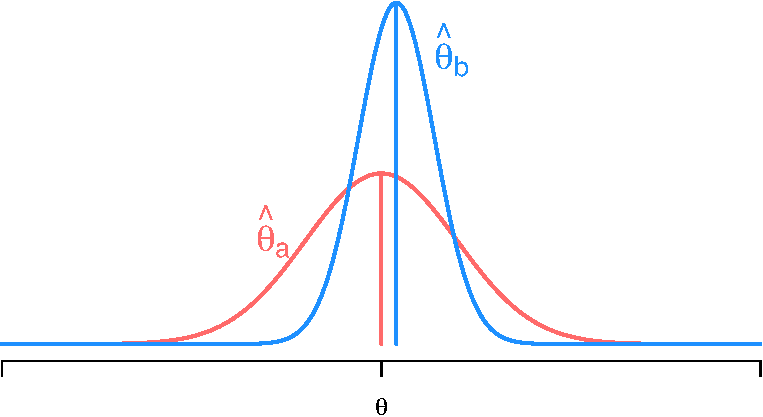
\includegraphics{estimation_files/figure-pdf/mse-1.pdf}

}

\caption{Two sampling distributions}

\end{figure}%

This figure shows the sampling distributions of two estimators: (1)
\(\widehat{\theta}_a\), which is unbiased (centered on the true value
\(\theta\)) but with a high sampling variance, and (2)
\(\widehat{\theta}_b\), which is slightly biased but with much lower
sampling variance. Even though \(\widehat{\theta}_b\) is biased, the
probability of drawing a value close to the truth is higher than for
\(\widehat{\theta}_a\). The MSE helps capture this balancing between
bias and variance, and, indeed, in this case,
\(MSE[\widehat{\theta}_b] < MSE[\widehat{\theta}_a]\).

\section{Summary}\label{summary-1}

In this chapter, we introduced \textbf{model-based inference}, in which
we posit a probability model for the data-generating process. These
models can be \textbf{parametric} in the sense that we specify the
probability distribution of the data up to some parameters. They can
also be \textbf{semiparametric} where we only specify certain features
of the distribution such as a finite mean and variance. This chapter
mostly focused on the latter, where we assumed the observed data were
\textbf{independent and identically distributed} draws from a population
distribution with finite mean and variance.

An \textbf{estimator} is a function of the data meant as a guess for
some quantity of interest in the population. Because it is a function of
random variables (the data), estimators are also random variables and
have distributions, called \textbf{sampling distributions}, across
repeated draws from the population. If this distribution is centered on
the true value of the quantity of interest, we call the estimator
\textbf{unbiased}. The variance of the sampling distribution, called the
\textbf{sampling variance}, tells us how variable we should expect the
estimator to be across draws from the population. The mean-squared error
is an overall measure of the accuracy of an estimator that combines
notions of bias and sampling variance.

We showed in this chapter that the sample mean is unbiased for the
population mean and that the sampling variance of the sample mean is the
ratio of the population variance to the sample size. We also saw that
\textbf{plug-in estimators} are a powerful way of constructing
estimators as functions of sample means. That said, the focus of this
chapter was finite-sample properties (that is, properties that are true
no matter the sample size). In the next chapter, we will derive even
more powerful results using large-sample approximations.

\chapter{Asymptotics}\label{sec-asymptotics}

\section{Introduction}\label{introduction-2}

Suppose we are still interested in estimating the proportion of citizens
who prefer increasing legal immigration. Based on the last chapter, a
good strategy would be to use the sample proportion of immigration
supporters in a random sample of citizens. You would have good reason to
be confident with this estimator, with its finite-sample properties like
unbiasedness and a sampling variance. We call these ``finite-sample''
properties since they hold at any sample size---they are as true for
random samples of size for \(n = 10\) as they are for random samples of
size \(n = 1,000,000\).

Finite-sample results, though, are of limited value because they only
tell us about the center and spread of the sampling distribution of
\(\Xbar_n\). Suppose we found that \(\Xbar_n = 0.47\) or 47\% of
respondents in a single survey supported increasing immigration. We
might want to know how plausible it would be for the true population
proportion -- which is distinct from the sample proportion -- to be 50\%
or greater. Questions like this are critical for a decision maker and,
to answer this, we need to know the (approximate) distribution of
\(\Xbar_n\) in addition to its mean and variance. We can often derive
the exact distribution of an estimator if we are willing to make
certain, sometimes strong assumptions about the underlying data (for
example, if the population is normal, then the sample means will also be
normal). Still, this approach is brittle: if our parametric assumption
is false, we are back to square one.

In this chapter, we take a different approach by asking what happens to
the sampling distribution of estimators as the sample size gets very
large, which we refer to as \textbf{asymptotic theory}. While
asymptotics will often simplify derivations, an essential point is that
everything we do with asymptotics will be an approximation. No one ever
has infinite data, but we hope that the approximations will be closer to
the truth as our samples get larger.

Asymptotic results are key to modern statistical methods because many
methods of quantifying uncertainty about estimates rely on asymptotic
approximations. We will rely on the asymptotic results we derive in this
chapter to estimate standard errors, construct confidence intervals, and
perform hypothesis tests, all without assuming a fully parametric model.

\section{Convergence of deterministic
sequences}\label{convergence-of-deterministic-sequences}

A helpful place to begin is by reviewing the basic idea of convergence
in deterministic sequences from calculus:

\begin{definition}[]\protect\hypertarget{def-limit}{}\label{def-limit}

A sequence \(\{a_n: n = 1, 2, \ldots\}\) has the \textbf{limit} \(a\)
written \(a_n \rightarrow a\) as \(n\rightarrow \infty\) or
\(\lim_{n\rightarrow \infty} a_n = a\) if for all \(\epsilon > 0\) there
is some \(n_{\epsilon} < \infty\) such that for all
\(n \geq n_{\epsilon}\), \(|a_n - a| \leq \epsilon\).

\end{definition}

We say that \(a_n\) \textbf{converges} to \(a\) if
\(\lim_{n\rightarrow\infty} a_n = a\). Basically, a sequence converges
to a number if the sequence gets closer and closer to that number as the
sequence goes on.

\begin{example}[]\protect\hypertarget{exm-limit}{}\label{exm-limit}

One important sequence that arises often in statistics is \(1/n\) as
\(n\to\infty\). It may seem clear that this sequence converges to 0, but
showing this using the formal definition of convergence is helpful.

Let us pick a specific value of \(\epsilon = 0.3\). Now we need to find
an integer \(n_{\epsilon}\) so that \(|1/n - 0| = 1/n \leq \epsilon\)
for all \(n \geq n_{\epsilon}\). Clearly, if \(\epsilon = 0.3\), then
\(n_{\epsilon} = 4\) would satisfy this condition since
\(1/4 \leq 0.3\).

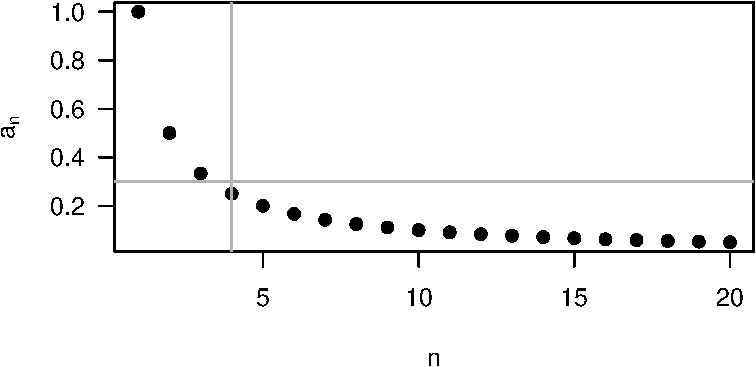
\includegraphics{asymptotics_files/figure-pdf/sequence-1.pdf}

More generally, for any \(\epsilon\), \(n \geq 1/\epsilon\) implies
\(1/n \leq \epsilon\). Thus, setting \(n_{\epsilon} = 1/\epsilon\)
ensures that the definition holds for all values of \(\epsilon\) and
that \(\lim_{n\to\infty} 1/n = 0\).

\end{example}

We will mostly not use such formal definitions to establish a limit but,
rather, rely on the properties of limits. For example, convergence and
limits follow basic arithmetic operations. Suppose that we have two
sequences with limits \(\lim_{n\to\infty} a_n = a\) and
\(\lim_{n\to\infty} b_n = b\). Then the properties of limits imply:

\begin{itemize}
\tightlist
\item
  \(\lim_{n\to\infty} (a_n + b_n) = a + b\)
\item
  \(\lim_{n\to\infty} a_nb_n = ab\)
\item
  \(\lim_{n\to\infty} ca_n = c\cdot a\)
\item
  \(\lim_{n\to\infty} (a_n/b_n) = a/b\) if \(b \neq 0\)
\item
  \(\lim_{n\to\infty} a_n^{k} = a^{k}\)
\end{itemize}

These rules plus the result in Example~\ref{exm-limit} allow us to prove
other useful facts such as \[
\lim_{n\to\infty} \frac{2}{n} = 2 \cdot 0 = 0 \qquad  \lim_{n\to\infty} \frac{1}{n^{2}} = 0.
\]

Can we apply a similar definition of convergence to sequences of random
variables (like estimators)? Possibly. Some examples clarify why this
might be difficult.\footnote{Due to Wasserman (2004), Chapter 5.}
Suppose we have a sequence of \(a_n = a\) for all \(n\) (that is, a
constant sequence). Then obviously
\(\lim_{n\rightarrow\infty} a_n = a\). Now let's say we have a sequence
of random variables, \(X_1, X_2, \ldots\), that are all independent with
a standard normal distribution, \(N(0,1)\). From the analogy to the
deterministic case, saying that \(X_n\) converges to \(X \sim N(0, 1)\)
would be tempting, but note that because they are all different random
variables, \(\P(X_n = X) = 0\). Thus, we must be careful about saying
how one variable converges to another variable.

Another example highlights subtle problems with a sequence of random
variables converging to a single value. Suppose we have a sequence of
random variables \(X_1, X_2, \ldots\) where \(X_n \sim N(0, 1/n)\).
Clearly, the distribution of \(X_n\) will concentrate around 0 for large
values of \(n\), so saying that \(X_n\) converges to 0 is tempting. But
notice that \(\P(X_n = 0) = 0\) because of the nature of continuous
random variables.

\section{Convergence in probability and
consistency}\label{convergence-in-probability-and-consistency}

A sequence of random variables can converge in several different ways.
The first type of convergence deals with sequences converging to a
single value.\footnote{Technically, a sequence can also converge in
  probability to another random variable, but the use case of converging
  to a single number is much more common in evaluating estimators.}

\begin{definition}[]\protect\hypertarget{def-inprob}{}\label{def-inprob}

A sequence of random variables, \(X_1, X_2, \ldots\), is said to
\textbf{converge in probability} to a value \(b\) if for every
\(\varepsilon > 0\), \[
\P(|X_n - b| > \varepsilon) \rightarrow 0,
\] as \(n\rightarrow \infty\). We write this \(X_n \inprob b\).

\end{definition}

What's happening in this definition? The even
\(|X_n - b| > \varepsilon\) says that a draw of \(X_n\) is more than
\(\varepsilon\) away from \(b\) (above or below). So convergence in
probability says that the probability of being some distance away from
the limit value goes to zero as the \(n\) goes to \(\infty\). With
deterministic sequences, we said that \(a_n\) converges to \(a\) as it
gets closer and closer to \(a\) as \(n\) gets bigger. For convergence in
probability, the sequence of random variables converges to \(b\) if the
probability that random variables are far away from \(b\) gets smaller
and smaller as \(n\) gets big.

\begin{example}[]\protect\hypertarget{exm-inprob}{}\label{exm-inprob}

Let's illustrate the definition of convergence in probability by
constructing a sequence of random variables, \[
X_n \sim N(0, 1/n).
\]

We can see intuitively that this sequence will be centered at zero with
a shrinking variance. Below, we will see that this is enough to
establish convergence in probability of \(X_n\) to 0, but we can also
show this in terms of its definition. To do so, we need to show that \[
\P(|X_n| > \varepsilon) \to 0.
\]

Let \(\Phi(\cdot)\) be the cdf for the standard normal. For any \(n\),
the cdf for \(X_n\) is \(\P(X_{n} < x) = \Phi(\sqrt{n}x)\). Thus, \[
\begin{aligned}
\P(|X_n| > \varepsilon) &= \P(X_n < -\varepsilon) + \P(X_n > \varepsilon) \\ &= \Phi(-\sqrt{n}\varepsilon) + (1 - \Phi(\sqrt{n}\varepsilon)) \to 0.
\end{aligned}
\] The last limit is due to \(\sqrt{n}\varepsilon \to \infty\) and thus,
by the properties of the cdf, \(\Phi(-\sqrt{n}\varepsilon) \to 0\) and
\(\Phi(\sqrt{n}\varepsilon) \to 1\). Clearly this holds for any
\(\varepsilon\), so \(X_n \inprob 0\).

\end{example}

\begin{tcolorbox}[enhanced jigsaw, toptitle=1mm, bottomrule=.15mm, leftrule=.75mm, rightrule=.15mm, breakable, colframe=quarto-callout-note-color-frame, title=\textcolor{quarto-callout-note-color}{\faInfo}\hspace{0.5em}{Notation alert}, colbacktitle=quarto-callout-note-color!10!white, titlerule=0mm, coltitle=black, left=2mm, colback=white, bottomtitle=1mm, opacitybacktitle=0.6, opacityback=0, toprule=.15mm, arc=.35mm]

Sometimes convergence in probability is written as
\(\text{plim}(Z_n) = b\) when \(Z_n \inprob b\), \(\text{plim}\) stands
for ``probability limit.''

\end{tcolorbox}

Convergence in probability is crucial for evaluating estimators. While
we said that unbiasedness was not the be-all and end-all of properties
of estimators, the following property is an essential and fundamental
property of good estimators.

\begin{definition}[]\protect\hypertarget{def-consistency}{}\label{def-consistency}

An estimator is \textbf{consistent} if
\(\widehat{\theta}_n \inprob \theta\).

\end{definition}

Consistency of an estimator implies that the sampling distribution of
the estimator ``collapses'' on the true value as the sample size gets
large. An estimator is \textbf{inconsistent} if it converges in
probability to any other value. As the sample size gets large, the
probability that an inconsistent estimator will be close to the truth
will approach 0. Generally speaking, consistency is a very desirable
property of an estimator.

\begin{tcolorbox}[enhanced jigsaw, toptitle=1mm, bottomrule=.15mm, leftrule=.75mm, rightrule=.15mm, breakable, colframe=quarto-callout-note-color-frame, title=\textcolor{quarto-callout-note-color}{\faInfo}\hspace{0.5em}{Note}, colbacktitle=quarto-callout-note-color!10!white, titlerule=0mm, coltitle=black, left=2mm, colback=white, bottomtitle=1mm, opacitybacktitle=0.6, opacityback=0, toprule=.15mm, arc=.35mm]

Estimators can be inconsistent yet still converge in probability to an
understandable quantity. For example, we will discuss in later chapters
that regression coefficients estimated by ordinary least squares (OLS)
are consistent for the conditional expectation if the conditional
expectation is linear. If that function is non-linear, however, then OLS
will be consistent for the best linear approximation to that function.
While not ideal, it does mean that this estimator is at least consistent
for an interpretable quantity.

\end{tcolorbox}

We can also define convergence in probability for a sequence of random
vectors, \(\X_1, \X_2, \ldots\), where
\(\X_i = (X_{i1}, \ldots, X_{ik})\) is a random vector of length \(k\).
This sequence converges in probability to a vector
\(\mb{b} = (b_1, \ldots, b_k)\) if and only if each random variable in
the vector converges to the corresponding element in \(\mb{b}\), or that
\(X_{nj} \inprob b_j\) for all \(j = 1, \ldots, k\).

\section{Useful inequalities}\label{useful-inequalities}

At first glance, establishing an estimator's consistency will be
difficult. How can we know if a distribution will collapse to a specific
value without knowing the shape or family of the distribution? It turns
out that there are certain relationships between the mean and variance
of a random variable and certain probability statements that hold for
all distributions (that have finite variance, at least). These
relationships are key to establishing results that do not depend on a
specific distribution.

\begin{theorem}[Markov
Inequality]\protect\hypertarget{thm-markov}{}\label{thm-markov}

For any r.v. \(X\) and any \(\delta >0\), \[
\P(|X| \geq \delta) \leq \frac{\E[|X|]}{\delta}.
\]

\end{theorem}

\begin{proof}
Note that we can let \(Y = |X|/\delta\) and rewrite the statement as
\(\P(Y \geq 1) \leq \E[Y]\) (since \(\E[|X|]/\delta = \E[|X|/\delta]\)
by the properties of expectation), which is what we will show. But also
note that \[
\mathbb{I}(Y \geq 1) \leq Y.
\] Why does this hold? The two possible values of the indicator function
show why. If \(Y\) is less than 1, then the indicator function will be
0, but recall that \(Y\) is nonnegative, so we know that it must be at
least as big as 0 so that inequality holds. If \(Y \geq 1\), then the
indicator function will take the value one, but we just said that
\(Y \geq 1\), so the inequality holds. If we take the expectation of
both sides of this inequality, we obtain the result (remember, the
expectation of an indicator function is the probability of the event).
\end{proof}

In words, Markov's inequality says that the probability of a random
variable being large in magnitude cannot be high if the average is not
large in magnitude. Blitzstein and Hwang (2019) provide an excellent
intuition behind this result using income as an example. Let \(X\) be
the income of a randomly selected individual in a population and set
\(\delta = 2\E[X]\) so that the inequality becomes
\(\P(X > 2\E[X]) < 1/2\) (assuming that all income is nonnegative).
Here, the inequality says that the share of the population with an
income twice the average must be less than 0.5 since if more than half
the population were making twice the average income, then the average
would have to be higher.

It's pretty astounding how general this result is since it holds for all
random variables. Of course, its generality comes at the expense of not
being very informative. If \(\E[|X|] = 5\), for instance, the inequality
tells us that \(\P(|X| \geq 1) \leq 5\), which is not very helpful since
we already know that probabilities are less than 1! We can get tighter
bounds if we are willing to make some assumptions about \(X\).

\begin{theorem}[Chebyshev
Inequality]\protect\hypertarget{thm-chebyshev}{}\label{thm-chebyshev}

Suppose that \(X\) is r.v. for which \(\V[X] < \infty\). Then, for every
real number \(\delta > 0\), \[
\P(|X-\E[X]| \geq \delta) \leq \frac{\V[X]}{\delta^2}.
\]

\end{theorem}

\begin{proof}
To prove this, we only need to square both sides of the inequality
inside the probability statement and apply Markov's inequality: \[
\P\left( |X - \E[X]| \geq \delta \right) = \P((X-\E[X])^2 \geq \delta^2) \leq \frac{\E[(X - \E[X])^2]}{\delta^2} = \frac{\V[X]}{\delta^2},
\] with the last equality holding by the definition of variance.
\end{proof}

Chebyshev's inequality is a straightforward extension of the Markov
result: the probability of a random variable being far from its mean
(that is, \(|X-\E[X]|\) being large) is limited by the variance of the
random variable. If we let \(\delta = c\sigma\), where \(\sigma\) is the
standard deviation of \(X\), we can use this result to bound the
normalized deviation from the mean: \[
\P\left(\frac{|X - \E[X]|}{\sigma} > c \right) \leq \frac{1}{c^2}.
\] This statement says the probability of being two standard deviations
away from the mean must be less than 1/4 = 0.25. Notice that this bound
can be fairly wide. If \(X\) has a normal distribution, we know that
about 5\% of draws will be greater than 2 SDs away from the mean, much
lower than the 25\% bound implied by Chebyshev's inequality.

\section{The law of large numbers}\label{the-law-of-large-numbers}

We can now use these inequalities to show how estimators can be
consistent for their target quantities of interest without making
parametric assumptions. Why are these inequalities helpful? Remember
that convergence in probability was about the probability of an
estimator being far away from a value going to zero. Chebyshev's
inequality shows that we can bound these exact probabilities.

The most famous consistency result has a special name.

\begin{theorem}[Weak Law of Large
Numbers]\protect\hypertarget{thm-lln}{}\label{thm-lln}

Let \(X_1, \ldots, X_n\) be i.i.d. draws from a distribution with mean
\(\mu = \E[X_i]\) and variance \(\sigma^2 = \V[X_i] < \infty\). Let
\(\Xbar_n = \frac{1}{n} \sum_{i =1}^n X_i\). Then,
\(\Xbar_n \inprob \mu\).

\end{theorem}

\begin{proof}
Recall that the sample mean is unbiased, so \(\E[\Xbar_n] = \mu\) with
sampling variance \(\sigma^2/n\). We can then apply Chebyshev to the
sample mean to get \[
\P(|\Xbar_n - \mu| \geq \delta) \leq \frac{\V[\Xbar_n]}{\delta} = \frac{\sigma^2}{n\delta^2}
\] An \(n\rightarrow\infty\), the right-hand side goes to 0, which means
that the left-hand side also must go to 0, which is the definition of
\(\Xbar_n\) converging in probability to \(\mu\).
\end{proof}

The weak law of large numbers (WLLN) shows that, under general
conditions, the sample mean gets closer to the population mean as
\(n\rightarrow\infty\). This result holds even when the variance of the
data is infinite, though researchers will rarely face such a situation.

\begin{tcolorbox}[enhanced jigsaw, toptitle=1mm, bottomrule=.15mm, leftrule=.75mm, rightrule=.15mm, breakable, colframe=quarto-callout-note-color-frame, title=\textcolor{quarto-callout-note-color}{\faInfo}\hspace{0.5em}{Note}, colbacktitle=quarto-callout-note-color!10!white, titlerule=0mm, coltitle=black, left=2mm, colback=white, bottomtitle=1mm, opacitybacktitle=0.6, opacityback=0, toprule=.15mm, arc=.35mm]

The naming of the ``weak'' law of large numbers seems to imply the
existence of a ``strong'' law of large numbers (SLLN), which is true.
The SLLN states that the sample mean converges to the population mean
with probability 1. This type of convergence, called \textbf{almost sure
convergence}, is stronger than convergence in probability, which only
says that the probability of the sample mean being close to the
population mean converges to 1. While it is nice to know that this
stronger form of convergence holds for the sample mean under the same
assumptions, it is rare for researchers outside of theoretical
probability and statistics to rely on almost sure convergence.

\end{tcolorbox}

\begin{example}[]\protect\hypertarget{exm-lln}{}\label{exm-lln}

Seeing how the distribution of the sample mean changes as a function of
the sample size allows us to appreciate the WLLN. We can see this by
taking repeated iid samples of different sizes from an exponential
random variable with rate parameter 0.5 so that \(\E[X_i] = 2\). In
Figure~\ref{fig-lln-sim}, we show the distribution of the sample mean
(across repeated samples) when the sample size is 15 (black), 30
(violet), 100 (blue), and 1000 (green). The sample mean distribution
``collapses'' on the true population mean, 2. The probability of being
far away from 2 becomes progressively smaller as the sample size
increases.

\begin{figure}[th]

\centering{

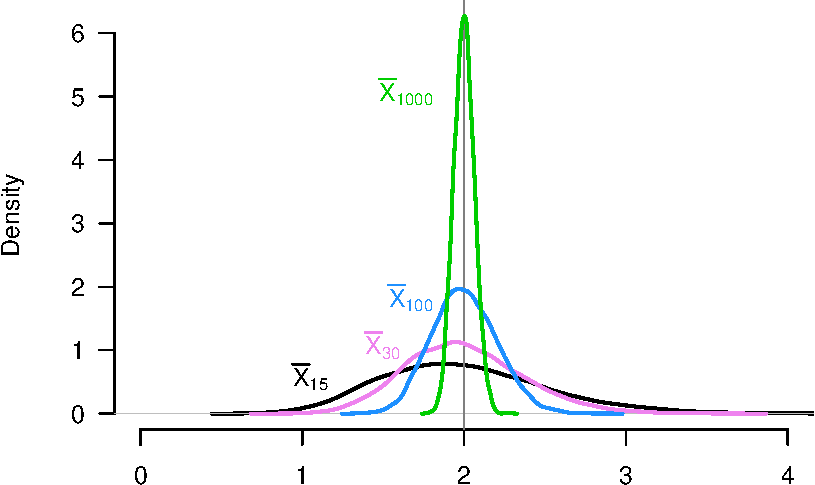
\includegraphics{asymptotics_files/figure-pdf/fig-lln-sim-1.pdf}

}

\caption{\label{fig-lln-sim}Sampling distribution of the sample mean as
a function of sample size.}

\end{figure}%

\end{example}

The WLLN also holds for random vectors in addition to random variables.
Let \((\X_1, \ldots, \X_n)\) be an iid sample of random vectors of
length \(k\), \(\mb{X}_i = (X_{i1}, \ldots, X_{ik})\). We can define the
vector sample mean as just the vector of sample means for each of the
entries:

\[
\overline{\mb{X}}_n = \frac{1}{n} \sum_{i=1}^n \mb{X}_i =
\begin{pmatrix}
\Xbar_{n,1} \\ \Xbar_{n,2} \\ \vdots \\ \Xbar_{n, k}
\end{pmatrix}
\] Since this is just a vector of sample means, each random variable in
the random vector will converge in probability to the mean of that
random variable. Fortunately, this is the exact definition of
convergence in probability for random vectors. We formally write this in
the following theorem.

\begin{theorem}[]\protect\hypertarget{thm-vector-wlln}{}\label{thm-vector-wlln}

If \(\X_i \in \mathbb{R}^k\) are iid draws from a distribution with
\(\E[X_{ij}] < \infty\) for all \(j=1,\ldots,k\) then as
\(n\rightarrow\infty\)

\[
\overline{\mb{X}}_n \inprob \E[\X] =
\begin{pmatrix}
\E[X_{i1}] \\ \E[X_{i2}] \\ \vdots \\ \E[X_{ik}]
\end{pmatrix}.
\]

\end{theorem}

\begin{tcolorbox}[enhanced jigsaw, toptitle=1mm, bottomrule=.15mm, leftrule=.75mm, rightrule=.15mm, breakable, colframe=quarto-callout-note-color-frame, title=\textcolor{quarto-callout-note-color}{\faInfo}\hspace{0.5em}{Notation alert}, colbacktitle=quarto-callout-note-color!10!white, titlerule=0mm, coltitle=black, left=2mm, colback=white, bottomtitle=1mm, opacitybacktitle=0.6, opacityback=0, toprule=.15mm, arc=.35mm]

Note that many of the formal results presented so far have ``moment
conditions'' that certain moments are finite. For the vector WLLN, we
saw that applied to the mean of each variable in the vector. Some books
use a shorthand for this: \(\E\Vert \X_i\Vert < \infty\), where \[
\Vert\X_i\Vert = \left(X_{i1}^2 + X_{i2}^2 + \ldots + X_{ik}^2\right)^{1/2}. 
\] This expression has slightly more compact notation, but why does it
work? One can show that this function, called the \textbf{Euclidean
norm} or \(L_2\)-norm, is a \textbf{convex} function, so we can apply
Jensen's inequality to show that: \[
\E\Vert \X_i\Vert \geq \Vert \E[\X_i] \Vert = (\E[X_{i1}]^2 + \ldots + \E[X_{ik}]^2)^{1/2}.
\] So if \(\E\Vert \X_i\Vert\) is finite, all the component means are
finite. Otherwise, the right-hand side of the previous equation would be
infinite.

\end{tcolorbox}

\section{Consistency of estimators}\label{consistency-of-estimators}

The WLLN shows that the sample mean of iid draws is consistent for the
population mean, which is a massive result given that so many estimators
are sample means of potentially complicated functions of the data. What
about other estimators? The proof of the WLLN points to one way to
determine that an estimator is consistent: if it is unbiased and the
sampling variance shrinks as the sample size grows.

\begin{theorem}[]\protect\hypertarget{thm-consis}{}\label{thm-consis}

For any estimator \(\widehat{\theta}_n\), if
\(\text{bias}[\widehat{\theta}_n] = 0\) and
\(\V[\widehat{\theta}_n] \rightarrow 0\) as \(n\rightarrow \infty\),
then \(\widehat{\theta}_n\) is consistent.

\end{theorem}

Thus, for unbiased estimators, if we can characterize its sampling
variance, we should be able to tell if it is consistent. This result is
handy since working with the probability statements used for the WLLN
can sometimes be confusing.

What about biased estimators? Consider a situation where we calculate
average household income, \(\Xbar_n\), from a random sample with mean
\(\mu\), but our actual interest is in the log of average income,
\(\alpha = \log(\mu)\). We can obviously use the standard plug-in
estimator \(\widehat{\alpha} = \log(\Xbar_n)\), but, for nonlinear
functions like logarithms we have
\(\log\left(\E[Z]\right) \neq \E[\log(Z)]\), so
\(\E[\widehat{\alpha}] \neq \log(\E[\Xbar_n])\) and the plug-in
estimator will be biased for \(\log(\mu)\). Obtaining an expression for
the bias in terms of \(n\) is also difficult. Is the quest doomed? Must
we give up on consistency? No, and, in fact, a few key properties of
consistency make working with it much easier compared to unbiasedness.

\begin{theorem}[Properties of convergence in
probability]\protect\hypertarget{thm-inprob-properties}{}\label{thm-inprob-properties}

Let \(X_n\) and \(Z_n\) be two sequences of random variables such that
\(X_n \inprob a\) and \(Z_n \inprob b\), and let \(g(\cdot)\) be a
continuous function. Then,

\begin{enumerate}
\def\labelenumi{\arabic{enumi}.}
\tightlist
\item
  \(g(X_n) \inprob g(a)\) (continuous mapping theorem)
\item
  \(X_n + Z_n \inprob a + b\)
\item
  \(X_nZ_n \inprob ab\)
\item
  \(X_n/Z_n \inprob a/b\) if \(b > 0\).
\end{enumerate}

\end{theorem}

We can now see that many of the nasty problems with expectations and
nonlinear functions are made considerably easier with convergence in
probability in the asymptotic setting. So while we know that
\(\log(\Xbar_n)\) is biased for \(\log(\mu)\), we know that it is
consistent since \(\log(\Xbar_n) \inprob \log(\mu)\) because \(\log\) is
a continuous function.

\begin{example}[]\protect\hypertarget{exm-nonresponse}{}\label{exm-nonresponse}

Suppose we implemented a survey by randomly selecting a sample from the
population of size \(n\), but not everyone responds to the survey. Let
the data consist of pairs of random variables,
\((Y_1, R_1), \ldots, (Y_n, R_n)\), where \(Y_i\) is the question of
interest and \(R_i\) is a binary indicator for if the respondent
answered the question (\(R_i = 1\)) or not (\(R_i = 0\)). Our goal is to
estimate the mean of the question for responders:
\(\E[Y_i \mid R_i = 1]\). We can use the law of iterated expectation to
obtain \[
\begin{aligned}
\E[Y_iR_i] &= \E[Y_i \mid R_i = 1]\P(R_i = 1) + \E[ 0 \mid R_i = 0]\P(R_i = 0) \\
\implies \E[Y_i \mid R_i = 1] &= \frac{\E[Y_iR_i]}{\P(R_i = 1)}
\end{aligned}
\]

The relevant estimator for this quantity is the mean of the outcome
among those who responded, which is slightly more complicated than a
typical sample mean because the denominator is a random variable: \[
\widehat{\theta}_n = \frac{\sum_{i=1}^n Y_iR_i}{\sum_{i=1}^n R_i}. 
\] Notice that this estimator is the ratio of two random variables. The
numerator has mean \(n\E[Y_iR_i]\) and the denominator has mean
\(n\P(R_i = 1)\). It is then tempting to say that we can take the ratio
of these means as the mean of \(\widehat{\theta}_n\), but expectations
are not preserved in nonlinear functions like this.

We can establish consistency of our estimator, though, by noting that we
can rewrite the estimator as a ratio of sample means \[
\widehat{\theta}_n = \frac{(1/n)\sum_{i=1}^n Y_iR_i}{(1/n)\sum_{i=1}^n R_i},
\] where by the WLLN the numerator
\((1/n)\sum_{i=1}^n Y_iR_i \inprob \E[Y_iR_i]\) and the denominator
\((1/n)\sum_{i=1}^n R_i \inprob \P(R_i = 1)\). Thus, by
Theorem~\ref{thm-inprob-properties}, we have \[
\widehat{\theta}_n = \frac{(1/n)\sum_{i=1}^n Y_iR_i}{(1/n)\sum_{i=1}^n R_i} \inprob \frac{\E[Y_iR_i]}{\P[R_i = 1]} = \E[Y_i \mid R_i = 1],
\] so long as the probability of responding is greater than zero. This
establishes that our sample mean among responders, while biased for the
conditional expectation among responders, is consistent for that
quantity.

\end{example}

Keeping the difference between unbiased and consistent clear in your
mind is essential. You can easily create ridiculous unbiased estimators
that are inconsistent. Let's return to our iid sample,
\(X_1, \ldots, X_n\), from a population with \(E[X_i] = \mu\). There is
nothing in the rule book against defining an estimator
\(\widehat{\theta}_{first} = X_1\) that uses the first observation as
the estimate. This estimator is silly, but it is unbiased since
\(\E[\widehat{\theta}_{first}] = \E[X_1] = \mu\). It is inconsistent
since the sampling variance of this estimator is just the variance of
the population distribution,
\(\V[\widehat{\theta}_{first}] = \V[X_i] = \sigma^2\), which does not
change as a function of the sample size. Generally speaking, we can
regard ``unbiased but inconsistent'' estimators as silly and not worth
our time (along with biased and inconsistent estimators).

Some estimators are biased but consistent that are often much more
interesting. We already saw one such estimator in
Example~\ref{exm-nonresponse}, but there are many more. Maximum
likelihood estimators, for example, are (under some regularity
conditions) consistent for the parameters of a parametric model but are
often biased.

To study these estimator, we can broaden Theorem~\ref{thm-consis} to the
class of \textbf{asymptotically unbiased} estimators that have bias that
vanishes as the sample size grows.

\begin{theorem}[]\protect\hypertarget{thm-consis-2}{}\label{thm-consis-2}

For any estimator \(\widehat{\theta}_n\), if
\(\text{bias}[\widehat{\theta}_n] \to 0\) and
\(\V[\widehat{\theta}_n] \rightarrow 0\) as \(n\rightarrow \infty\),
then \(\widehat{\theta}_n\) is consistent.

\end{theorem}

\begin{proof}
Using Markov's inequality, we have \[
\P\left( |\widehat{\theta}_n - \theta| \geq \delta \right) = \P((\widehat{\theta}_n-\theta)^2 \geq \delta^2) \leq \frac{\E[(\widehat{\theta}_n - \theta)^2]}{\delta^2} = \frac{\text{bias}[\widehat{\theta}_n]^2 + \V[\widehat{\theta}]}{\delta^2} \to 0.
\] The last inequality follows from the bias-variance decomposition of
the mean squared error in Equation~\ref{eq-mse-decomposition}.
\end{proof}

We can use this result to show consistency for a large range of
estimators.

\begin{example}[Plug-in variance
estimator]\protect\hypertarget{exm-plug-in-variance}{}\label{exm-plug-in-variance}

In the last chapter, we introduced the plug-in estimator for the
population variance, \[
\widehat{\sigma}^2 = \frac{1}{n} \sum_{i=1}^n (X_i - \Xbar_n)^2,
\] which we will now show is biased but consistent. To see the bias note
that we can rewrite the sum of square deviations
\[\sum_{i=1}^n (X_i - \Xbar_n)^2 = \sum_{i=1}^n X_i^2 - n\Xbar_n^2. \]
Then, the expectation of the plug-in estimator is \[
\begin{aligned}
\E[\widehat{\sigma}^2] & = \E\left[\frac{1}{n}\sum_{i=1}^n X_i^2\right] - \E[\Xbar_n^2] \\
&= \E[X_i^2] - \frac{1}{n^2}\sum_{i=1}^n \sum_{j=1}^n \E[X_iX_j] \\
&= \E[X_i^2] - \frac{1}{n^2}\sum_{i=1}^n \E[X_i^2] - \frac{1}{n^2}\sum_{i=1}^n \sum_{j\neq i} \underbrace{\E[X_i]\E[X_j]}_{\text{independence}} \\
&= \E[X_i^2] - \frac{1}{n}\E[X_i^2] - \frac{1}{n^2} n(n-1)\mu^2 \\
&= \frac{n-1}{n} \left(\E[X_i^2] - \mu^2\right) \\
&= \frac{n-1}{n} \sigma^2 = \sigma^2 - \frac{1}{n}\sigma^2
\end{aligned}. 
\] Thus, we can see that the bias of the plug-in estimator is
\(-(1/n)\sigma^2\), so it slightly underestimates the variance. Nicely,
though, the bias shrinks as a function of the sample size, so according
to Theorem~\ref{thm-consis-2}, it will be consistent so long as the
sampling variance of \(\widehat{\sigma}^2\) shrinks as a function of the
sample size, which it does (though omit that proof here). Of course,
simply multiplying this estimator by \(n/(n-1)\) will give an unbiased
and consistent estimator that is also the typical sample variance
estimator.

\end{example}

\section{Convergence in distribution and the central limit
theorem}\label{convergence-in-distribution-and-the-central-limit-theorem}

Convergence in probability and the law of large numbers are beneficial
for understanding how our estimators will (or will not) collapse to
their estimand as the sample size increases. But what about the shape of
the sampling distribution of our estimators? For statistical inference,
we would like to be able to make probability statements such as
\(\P(a \leq \widehat{\theta}_n \leq b)\). These statements will be the
basis of hypothesis testing and confidence intervals. But to make those
types of statements, we need to know the entire distribution of
\(\widehat{\theta}_n\), not just the mean and variance. Luckily,
established results will allow us to approximate the sampling
distribution of a vast swath of estimators when our sample sizes are
large.

We need first to describe a weaker form of convergence to see how we
will develop these approximations.

\begin{definition}[]\protect\hypertarget{def-indist}{}\label{def-indist}

Let \(X_1,X_2,\ldots\), be a sequence of r.v.s, and for
\(n = 1,2, \ldots\) let \(F_n(x)\) be the c.d.f. of \(X_n\). Then it is
said that \(X_1, X_2, \ldots\) \textbf{converges in distribution} to
r.v. \(X\) with c.d.f. \(F(x)\) if \[
\lim_{n\rightarrow \infty} F_n(x) = F(x),
\] for all values of \(x\) for which \(F(x)\) is continuous. We write
this as \(X_n \indist X\) or sometimes \(X_n ⇝ X\).

\end{definition}

Essentially, convergence in distribution means that as \(n\) gets large,
the distribution of \(X_n\) becomes more and more similar to the
distribution of \(X\), which we often call the \textbf{asymptotic
distribution} of \(X_n\) (other names include the \textbf{large-sample
distribution}). If we know that \(X_n \indist X\), then we can use the
distribution of \(X\) as an approximation to the distribution of
\(X_n\), and that distribution can be reasonably accurate.

\begin{example}[]\protect\hypertarget{exm-indist}{}\label{exm-indist}

A simple example of convergence in distribution would be the sequence \[
X_n \sim N\left(\frac{1}{n}, 1 + \frac{1}{n}\right),
\] which, of course, has the cdf, \[
\Phi\left(\frac{x - 1/n}{1+1/n}\right).
\] By inspection, this converges to \(\Phi(x)\), which is the cdf for
the standard normal. This implies \(X_n \indist N(0, 1)\).

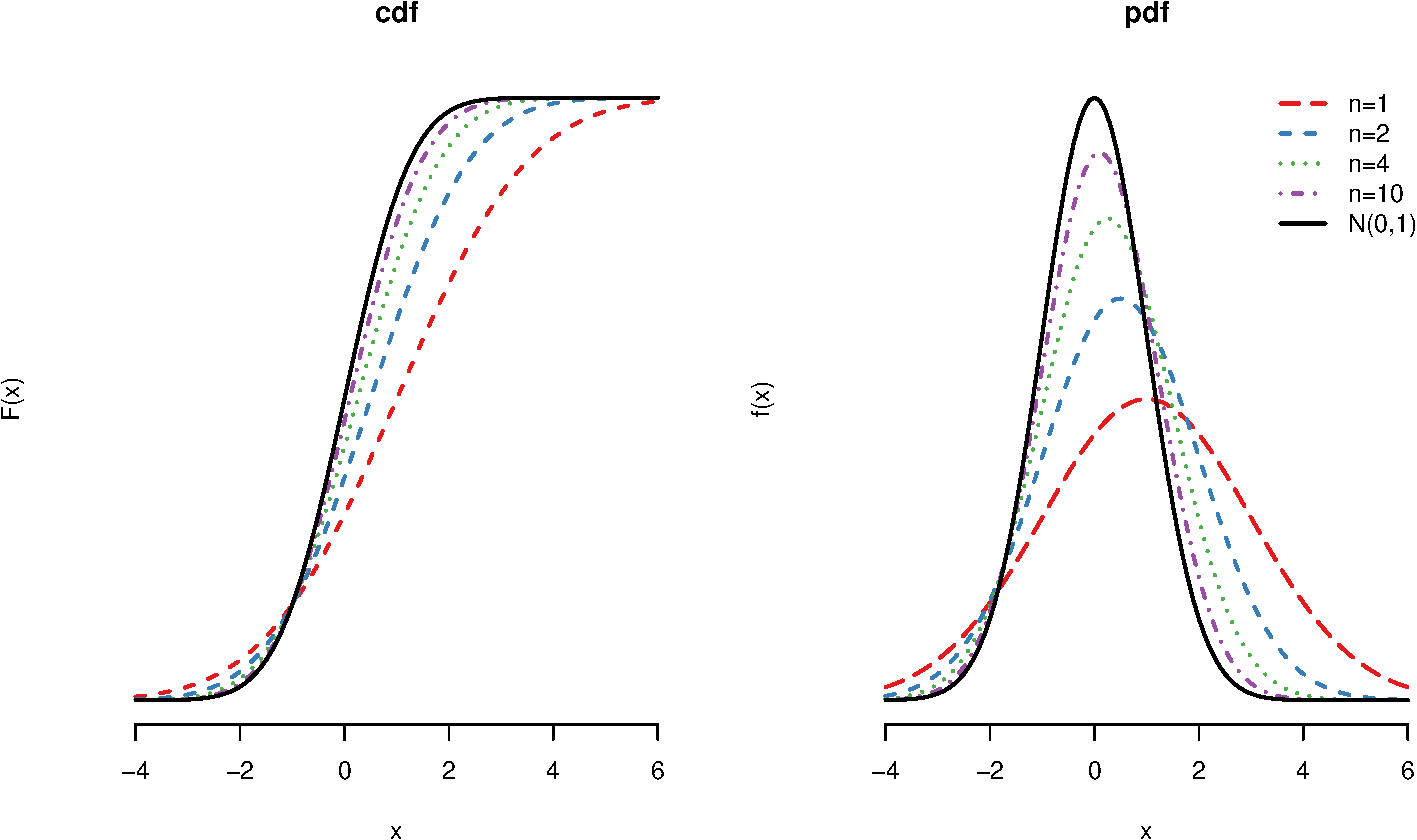
\includegraphics{asymptotics_files/figure-pdf/indist-1.pdf}

\end{example}

One of the most remarkable results in probability and statistics is that
a large class of estimators will converge in distribution to one
particular family of distributions: the normal. This result is one
reason we study the normal so much and why investing in building
intuition about it will pay off across many domains of applied work. We
call this broad class of results the ``central limit theorem'' (CLT),
but it would probably be more accurate to refer to them as ``central
limit theorems'' since much of statistics is devoted to showing the
result in different settings. We now present the simplest CLT for the
sample mean.

\begin{theorem}[Central Limit
Theorem]\protect\hypertarget{thm-clt}{}\label{thm-clt}

Let \(X_1, \ldots, X_n\) be i.i.d. r.v.s from a distribution with mean
\(\mu = \E[X_i]\) and variance \(\sigma^2 = \V[X_i]\). Then if
\(\E[X_i^2] < \infty\), we have \[
\frac{\Xbar_n - \mu}{\sqrt{\V[\Xbar_n]}} = \frac{\sqrt{n}\left(\Xbar_n - \mu\right)}{\sigma} \indist \N(0, 1).
\]

\end{theorem}

In words: the sample mean of a random sample from a population with
finite mean and variance will be approximately normally distributed in
large samples. Notice how we have not made any assumptions about the
distribution of the underlying random variables, \(X_i\). They could be
binary, event count, continuous, or anything. The CLT is incredibly
broadly applicable.

\begin{tcolorbox}[enhanced jigsaw, toptitle=1mm, bottomrule=.15mm, leftrule=.75mm, rightrule=.15mm, breakable, colframe=quarto-callout-note-color-frame, title=\textcolor{quarto-callout-note-color}{\faInfo}\hspace{0.5em}{Notation alert}, colbacktitle=quarto-callout-note-color!10!white, titlerule=0mm, coltitle=black, left=2mm, colback=white, bottomtitle=1mm, opacitybacktitle=0.6, opacityback=0, toprule=.15mm, arc=.35mm]

Why do we state the CLT in terms of the sample mean after centering and
scaling by its standard error? Suppose we don't normalize the sample
mean in this way. In that case, it isn't easy to talk about convergence
in distribution because we know from the WLLN that
\(\Xbar_n \inprob \mu\), so in the limit, the distribution of
\(\Xbar_n\) is concentrated at point mass around that value. Normalizing
by centering and rescaling ensures that the variance of the resulting
quantity will not depend on \(n\), so it makes sense to talk about its
distribution converging. Sometimes you will see the equivalent result as
\[
\sqrt{n}\left(\Xbar_n - \mu\right) \indist \N(0, \sigma^2).
\]

\end{tcolorbox}

We can use this result to state approximations that we can use when
discussing estimators such as \[
\Xbar_n \overset{a}{\sim} N(\mu, \sigma^2/n),
\] where we use \(\overset{a}{\sim}\) to be ``approximately distributed
as in large samples.'' This approximation allows us to say things like:
``in large samples, we should expect the sample mean to between within
\(2\sigma/\sqrt{n}\) of the true mean in 95\% of repeated samples.''
These statements will be essential for hypothesis tests and confidence
intervals! Estimators so often follow the CLT that we have an expression
for this property.

\begin{definition}[]\protect\hypertarget{def-asymptotically-normal}{}\label{def-asymptotically-normal}

An estimator \(\widehat{\theta}_n\) is \textbf{asymptotically normal} if
for some \(\theta\) \[
\sqrt{n}\left( \widehat{\theta}_n - \theta \right) \indist N\left(0,\V_{\theta}\right).
\]

\end{definition}

\begin{example}[]\protect\hypertarget{exm-bin-clt}{}\label{exm-bin-clt}

To illustrate how the CLT works, we can simulate the sampling
distribution of the (normalized) sample mean at different sample sizes.
Let \(X_1, \ldots, X_n\) be iid samples from a Bernoulli with
probability of success 0.25. We then draw repeated samples of size
\(n=30\) and \(n=100\) and calculate \(\sqrt{n}(\Xbar_n - 0.25)/\sigma\)
for each random sample. Figure~\ref{fig-clt} plots the density of these
two sampling distributions along with a standard normal reference. We
can see that even at \(n=30\), the rough shape of the density looks
normal, with spikes and valleys due to the discrete nature of the data
(the sample mean can only take on 31 possible values in this case). By
\(n=100\), the sampling distribution is very close to the true standard
normal.

\begin{figure}[th]

\centering{

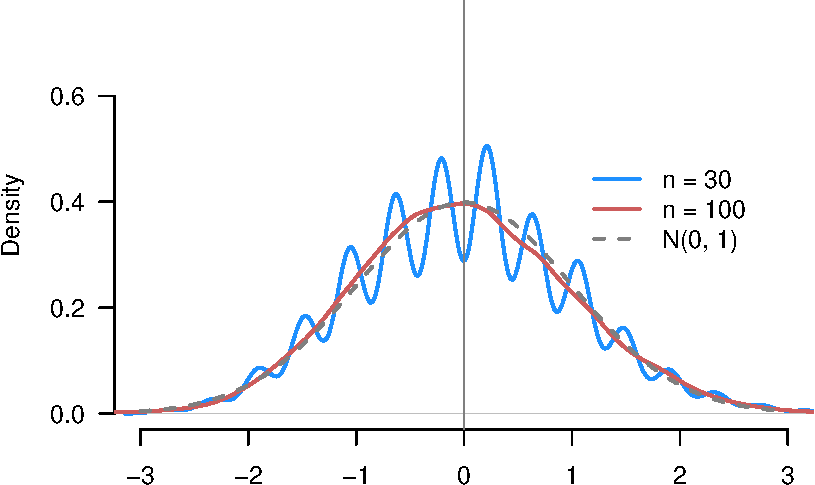
\includegraphics{asymptotics_files/figure-pdf/fig-clt-1.pdf}

}

\caption{\label{fig-clt}Sampling distributions of the normalized sample
mean at n=30 and n=100.}

\end{figure}%

\end{example}

There are several properties of convergence in distribution that are
helpful to us.

\begin{theorem}[Properties of convergence in
distribution]\protect\hypertarget{thm-indist-properties}{}\label{thm-indist-properties}

Let \(X_n\) be a sequence of random variables \(X_1, X_2,\ldots\) that
converges in distribution to some rv \(X\) and let \(Y_n\) be a sequence
of random variables \(Y_1, Y_2,\ldots\) that converges in probability to
some number, \(c\). Then,

\begin{enumerate}
\def\labelenumi{\arabic{enumi}.}
\tightlist
\item
  \(g(X_n) \indist g(X)\) for all continuous functions \(g\).
\item
  \(X_nY_n\) converges in distribution to \(cX\)
\item
  \(X_n + Y_n\) converges in distribution to \(X + c\)
\item
  \(X_n / Y_n\) converges in distribution to \(X / c\) if \(c \neq 0\)
\end{enumerate}

\end{theorem}

We refer to the last three results as \textbf{Slutsky's theorem}. These
results are often crucial for determining an estimator's asymptotic
distribution.

A critical application of Slutsky's theorem is when we replace the
(unknown) population variance in the CLT with an estimate. Recall the
definition of the \textbf{sample variance} as \[
S_n^2 = \frac{1}{n-1} \sum_{i=1}^n (X_i - \Xbar_n)^2,
\] with the \textbf{sample standard deviation} defined as
\(S_{n} = \sqrt{S_{n}^2}\). It's easy to show that these are consistent
estimators for their respective population parameters \[ 
S_{n}^2 \inprob \sigma^2 = \V[X_i], \qquad S_{n} \inprob \sigma,
\] which, by Slutsky's theorem, implies that \[
\frac{\sqrt{n}\left(\Xbar_n - \mu\right)}{S_n} \indist \N(0, 1)
\] Comparing this result to the statement of CLT, we see that replacing
the population variance with a consistent estimate of the variance (or
standard deviation) does not affect the asymptotic distribution.

Like with the WLLN, the CLT holds for random vectors of sample means,
where their centered and scaled versions converge to a multivariate
normal distribution with a covariance matrix equal to the covariance
matrix of the underlying random vectors of data, \(\X_i\).

\begin{theorem}[]\protect\hypertarget{thm-multivariate-clt}{}\label{thm-multivariate-clt}

If \(\mb{X}_i \in \mathbb{R}^k\) are i.i.d. and
\(\E\Vert \mb{X}_i \Vert^2 < \infty\), then as \(n \to \infty\), \[
\sqrt{n}\left( \overline{\mb{X}}_n - \mb{\mu}\right) \indist \N(0, \mb{\Sigma}),
\] where \(\mb{\mu} = \E[\mb{X}_i]\) and
\(\mb{\Sigma} = \V[\mb{X}_i] = \E\left[(\mb{X}_i-\mb{\mu})(\mb{X}_i - \mb{\mu})'\right]\).

\end{theorem}

Notice that \(\mb{\mu}\) is the vector of population means for all the
random variables in \(\X_i\) and \(\mb{\Sigma}\) is the
variance-covariance matrix for that vector.

\begin{tcolorbox}[enhanced jigsaw, toptitle=1mm, bottomrule=.15mm, leftrule=.75mm, rightrule=.15mm, breakable, colframe=quarto-callout-note-color-frame, title=\textcolor{quarto-callout-note-color}{\faInfo}\hspace{0.5em}{Note}, colbacktitle=quarto-callout-note-color!10!white, titlerule=0mm, coltitle=black, left=2mm, colback=white, bottomtitle=1mm, opacitybacktitle=0.6, opacityback=0, toprule=.15mm, arc=.35mm]

As with the notation alert with the WLLN, we are using shorthand here,
\(\E\Vert \mb{X}_i \Vert^2 < \infty\), which implies that
\(\E[X_{ij}^2] < \infty\) for all \(j = 1,\ldots, k\), or equivalently,
that the variances of each variable in the sample means has finite
variance.

\end{tcolorbox}

\section{Confidence intervals}\label{confidence-intervals}

We now turn to an essential application of the central limit theorem:
confidence intervals.

Suppose we have run an experiment with a treatment and control group and
have presented readers with our single best guess about the treatment
effect using the difference in sample means. We have also presented the
estimated standard error of this estimate to give readers a sense of how
variable it is. But none of these approaches answer a fairly compelling
question: what range of values of the treatment effect is
\textbf{plausible} given the data we observe?

A point estimate of the difference in sample means typically has 0
probability of being the exact true value, but intuitively we hope that
the true treatment effect is close to our estimate. \textbf{Confidence
intervals} make this kind of intuition more formal by instead estimating
ranges of values with a fixed percentage of these ranges containing the
actual unknown parameter value.

We begin with the basic definition of a confidence interval.

\begin{definition}[]\protect\hypertarget{def-coverage}{}\label{def-coverage}

A \(1-\alpha\) \textbf{confidence interval} for a real-valued parameter
\(\theta\) is a pair of statistics \(L= L(X_1, \ldots, X_n)\) and
\(U = U(X_1, \ldots, X_n)\) such that \(L < U\) for all values of the
sample and such that \[ 
\P(L \leq \theta \leq U \mid \theta) \geq 1-\alpha, \quad \forall \theta \in \Theta.
\]

\end{definition}

We say that a \(1-\alpha\) confidence interval covers (or contains,
captures, traps, etc.) the true value at least \(100(1-\alpha)\%\) of
the time, and we refer to \(1-\alpha\) as the \textbf{coverage
probability} or simply \textbf{coverage}. Typical confidence intervals
include 95\% percent (\(\alpha = 0.05\)), 90\% (\(\alpha = 0.1\)), and
99\% (\(\alpha = 0.01\)). All else equal, larger coverage will imply
larger intervals.

So a confidence interval is a random interval with a particular
guarantee about how often it will contain the true value of the unknown
population parameter (in our example, the true treatment effect).
Remember what is random and what is fixed in this setup. The interval
varies from sample to sample, but the true value of the parameter stays
fixed even if it is unknown, and the coverage is how often we should
expect the interval to contain that true value. The ``repeating my
sample over and over again'' analogy can break down very quickly, so it
is sometimes helpful to interpret it as giving guarantees across
confidence intervals across different experiments. In particular,
suppose that a journal publishes 100 quantitative articles annually,
each producing a single 95\% confidence interval for their quantity of
interest. Then, if the confidence intervals are valid and each is
constructed in the exact same way, we should expect 95 of those
confidence intervals to contain the true value.

\begin{tcolorbox}[enhanced jigsaw, toptitle=1mm, bottomrule=.15mm, leftrule=.75mm, rightrule=.15mm, breakable, colframe=quarto-callout-warning-color-frame, title=\textcolor{quarto-callout-warning-color}{\faExclamationTriangle}\hspace{0.5em}{Warning}, colbacktitle=quarto-callout-warning-color!10!white, titlerule=0mm, coltitle=black, left=2mm, colback=white, bottomtitle=1mm, opacitybacktitle=0.6, opacityback=0, toprule=.15mm, arc=.35mm]

Suppose we have a 95\% confidence interval, \([0.1, 0.4]\). It would be
tempting to make a probability statement like
\(\P(0.1 \leq \theta \leq 0.4 \mid \theta) = 0.95\) or that there's a
95\% chance that the parameter is in \([0.1, 0.4]\). But looking at the
probability statement, everything on the left-hand side of the
conditioning bar is fixed, so the probability either has to be 0
(\(\theta\) is outside the interval) or 1 (\(\theta\) is in the
interval); the unknown parameter is a fixed value, so it is either in
the interval or it is not. Another way to think about this is that the
coverage probability of a confidence interval refers to its status as a
pair of random variables, \((L, U)\), not any particular realization of
those variables like \((0.1, 0.4)\). As an analogy, consider if we
calculated the sample mean as \(0.25\) and then tried to say that
\(0.25\) is unbiased for the population mean. This statement doesn't
make sense because unbiasedness refers not to a fixed value but how the
sample mean varies from sample to sample.

\end{tcolorbox}

In most cases, we will not be able to derive exact confidence intervals
but rather confidence intervals that are \textbf{asymptotically valid},
which means that if we write the interval as a function of the sample
size, \((L_n, U_n)\), they would have \textbf{asymptotic coverage} \[
\lim_{n\to\infty} \P(L_n \leq \theta \leq U_n) \geq 1-\alpha \quad\forall\theta\in\Theta.
\]

We can show asymptotic coverage for most confidence intervals since we
usually rely on large-sample approximations based on the central limit
theorem.

\subsection{Deriving confidence
intervals}\label{deriving-confidence-intervals}

To derive confidence intervals, consider the standard formula for the
95\% confidence interval of the sample mean, \[ 
\left[\Xbar_n - 1.96\frac{s}{\sqrt{n}},\; \Xbar_n + 1.96\frac{s}{\sqrt{n}}\right],
\] where \(s\) is the sample standard deviation and \(s/\sqrt{n}\) is
the estimate of the standard error of the sample mean. If this is a 95\%
confidence interval, then the probability that it contains the true
population mean \(\mu\) should be 0.95, but how can we derive this? We
can justify this logic using the central limit theorem, and the argument
will hold for any asymptotically normal estimator.

Suppose we have an estimator, \(\widehat{\theta}_n\) for the parameter
\(\theta\) with estimated standard error
\(\widehat{\se}[\widehat{\theta}_n]\). If the estimator is
asymptotically normal, then in large samples, we know that \[ 
\frac{\widehat{\theta}_n - \theta}{\widehat{\se}[\widehat{\theta}_n]} \sim \N(0, 1).
\] Then we use our knowledge of the standard normal to find \[ 
\P\left( -1.96 \leq \frac{\widehat{\theta}_n - \theta}{\widehat{\se}[\widehat{\theta}_n]} \leq 1.96\right) = 0.95.
\] Multiplying each part of the inequality by
\(\widehat{\se}[\widehat{\theta}_n]\) gives us \[ 
\P\left( -1.96\,\widehat{\se}[\widehat{\theta}_n] \leq \widehat{\theta}_n - \theta \leq 1.96\,\widehat{\se}[\widehat{\theta}_n]\right) = 0.95,
\] We then subtract all parts by the estimator to get \[ 
\P\left(-\widehat{\theta}_n - 1.96\,\widehat{\se}[\widehat{\theta}_n] \leq - \theta \leq -\widehat{\theta}_n + 1.96\,\widehat{\se}[\widehat{\theta}_n]\right) = 0.95,
\] and finally we multiply all parts by \(-1\) (and flipping the
inequalities) to arrive at \[ 
\P\left(\widehat{\theta}_n - 1.96\,\widehat{\se}[\widehat{\theta}_n] \leq \theta \leq \widehat{\theta}_n + 1.96\,\widehat{\se}[\widehat{\theta}_n]\right) = 0.95.
\] To connect back to the definition of the confidence interval, we have
now shown that the random interval \([L, U]\) where \[ 
\begin{aligned}
  L = L(X_1, \ldots, X_n) &= \widehat{\theta}_n - 1.96\,\widehat{\se}[\widehat{\theta}_n] \\
  U = U(X_1, \ldots, X_n) &= \widehat{\theta}_n + 1.96\,\widehat{\se}[\widehat{\theta}_n],
\end{aligned}
\] is an asymptotically valid estimator.\footnote{The analysis here
  largely comes from Senn (2012).} Replacing \(\Xbar_n\) for
\(\widehat{\theta}_n\) and \(s/\sqrt{n}\) for
\(\widehat{\se}[\widehat{\theta}_n]\) establishes how the standard 95\%
confidence interval for the sample mean above is asymptotically valid.

\begin{figure}[th]

\centering{

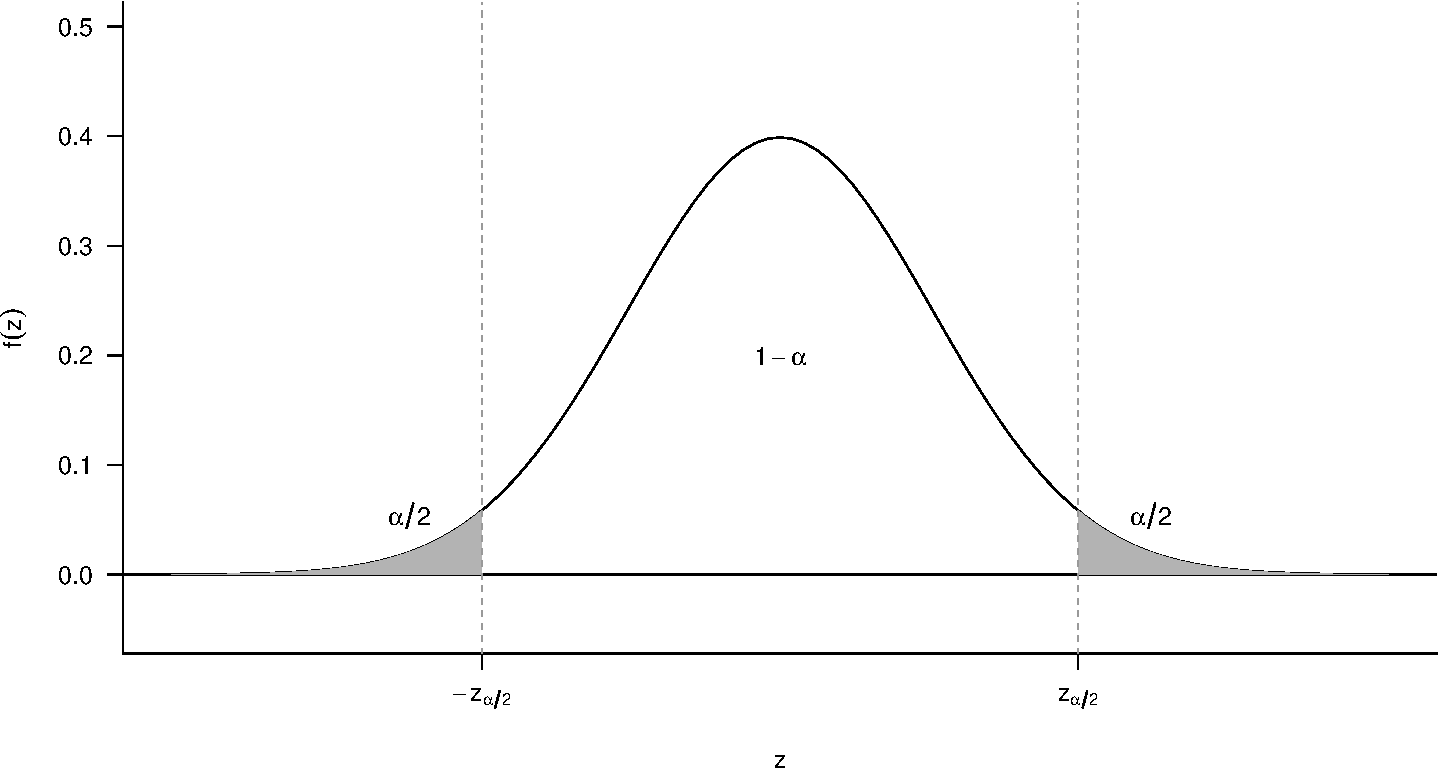
\includegraphics{asymptotics_files/figure-pdf/fig-std-normal-1.pdf}

}

\caption{\label{fig-std-normal}Critical values for the standard normal.}

\end{figure}%

How can we generalize this to \(1-\alpha\) confidence intervals? For a
random variable that is distributed following a standard normal, \(Z\),
we know that \[ 
\P(-z_{\alpha/2} \leq Z \leq z_{\alpha/2}) = 1-\alpha
\] which implies that we can obtain a \(1-\alpha\) asymptotic confidence
intervals by using the interval \([L, U]\), where \[ 
L = \widehat{\theta}_{n} - z_{\alpha/2} \widehat{\se}[\widehat{\theta}_{n}], \quad U = \widehat{\theta}_{n} + z_{\alpha/2} \widehat{\se}[\widehat{\theta}_{n}]. 
\] This is sometimes shortened to
\(\widehat{\theta}_n \pm z_{\alpha/2} \widehat{\se}[\widehat{\theta}_{n}]\).
Remember that we can obtain the values of \(z_{\alpha/2}\) easily from
R:

\begin{Shaded}
\begin{Highlighting}[]
\DocumentationTok{\#\# alpha = 0.1 for 90\% CI}
\FunctionTok{qnorm}\NormalTok{(}\FloatTok{0.1} \SpecialCharTok{/} \DecValTok{2}\NormalTok{, }\AttributeTok{lower.tail =} \ConstantTok{FALSE}\NormalTok{)}
\end{Highlighting}
\end{Shaded}

\begin{verbatim}
[1] 1.644854
\end{verbatim}

As a concrete example, then, we could derive a 90\% asymptotic
confidence interval for the sample mean as \[ 
\left[\Xbar_{n} - 1.64 \frac{\widehat{\sigma}}{\sqrt{n}}, \Xbar_{n} + 1.64 \frac{\widehat{\sigma}}{\sqrt{n}}\right]
\]

\subsection{Interpreting confidence
intervals}\label{interpreting-confidence-intervals}

A very important point is that the interpretation of confidence is how
the random interval performs over repeated samples. A valid 95\%
confidence interval is a random interval that contains the true
population value in 95\% of samples. Simulating repeated samples helps
clarify this.

\begin{example}[]\protect\hypertarget{exm-cis}{}\label{exm-cis}

Suppose we are taking samples of size \(n=500\) of random variables
where \(X_i \sim \N(1, 10)\), and we want to estimate the population
mean \(\E[X] = 1\). To do so, we repeat the following steps:

\begin{enumerate}
\def\labelenumi{\arabic{enumi}.}
\tightlist
\item
  Draw a sample of \(n=500\) from \(\N(1, 10)\).
\item
  Calculate the 95\% confidence interval sample mean
  \(\Xbar_n \pm 1.96\widehat{\sigma}/\sqrt{n}\).
\item
  Plot the intervals along the x-axis and color them blue if they
  contain the truth (1) and red if not.
\end{enumerate}

Figure~\ref{fig-ci-sim} shows 100 iterations of these steps. We see
that, as expected, most calculated CIs do contain the true value. Five
random samples produce intervals that fail to include 1, an exact
coverage rate of 95\%. Of course, this is just one simulation, and a
different set of 100 random samples might have produced a slightly
different coverage rate. The guarantee of the 95\% confidence intervals
is that if we were to continue to take these repeated samples, the
long-run frequency of intervals covering the truth would approach 0.95.

\begin{figure}[th]

\centering{

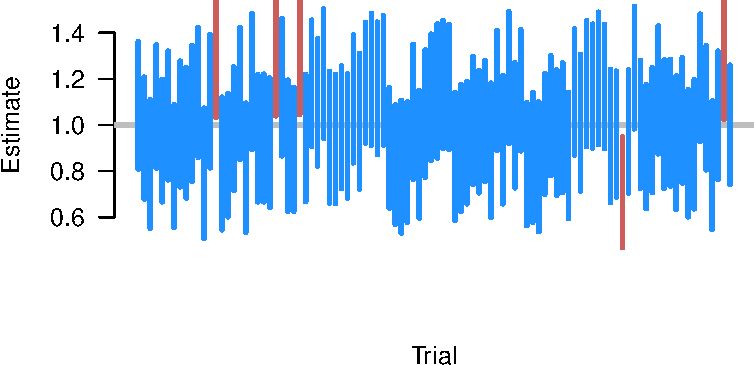
\includegraphics{asymptotics_files/figure-pdf/fig-ci-sim-1.pdf}

}

\caption{\label{fig-ci-sim}95\% confidence intervals from 100 random
samples. Intervals are blue if they contain the truth and red if they do
not.}

\end{figure}%

\end{example}

\section{Delta method}\label{sec-delta-method}

Suppose that we know that an estimator follows the CLT, and so we have
\[
\sqrt{n}\left(\widehat{\theta}_n - \theta \right) \indist \N(0, V),
\] but we actually want to estimate \(h(\theta)\) so we use the plug-in
estimator, \(h(\widehat{\theta}_n)\). It seems like we should be able to
apply part 1 of Theorem~\ref{thm-indist-properties} to obtain the
asymptotic distribution of \(h(\widehat{\theta}_n)\). Still, the CLT
established the large-sample distribution of the centered and scaled
random sequence, \(\sqrt{n}(\widehat{\theta}_n - \theta)\), not to the
original estimator itself, and we would need the latter to investigate
the asymptotic distribution of \(h(\widehat{\theta}_n)\). We can use a
little bit of calculus to get an approximation of the distribution we
need.

\begin{theorem}[]\protect\hypertarget{thm-delta-method}{}\label{thm-delta-method}

If \(\sqrt{n}\left(\widehat{\theta}_n - \theta\right) \indist \N(0, V)\)
and \(h(u)\) is continuously differentiable in a neighborhood around
\(\theta\), then as \(n\to\infty\), \[
\sqrt{n}\left(h(\widehat{\theta}_n) - h(\theta) \right) \indist \N(0, (h'(\theta))^2 V).
\]

\end{theorem}

Understanding what is happening here provides intuition as to when this
might go wrong. Why do we focus on continuously differentiable
functions, \(h()\)? These functions can be well-approximated with a line
in a neighborhood around a given point like \(\theta\). In
Figure~\ref{fig-delta}, we show this at the point where the tangent line
at \(\theta_0\), which has slope \(h'(\theta_0)\), is very similar to
\(h(\theta)\) for values close to \(\theta_0\). Because of this, we can
approximate the difference between \(h(\widehat{\theta}_n)\) and
\(h(\theta_0)\) with the what this tangent line would give us: \[
\underbrace{\left(h(\widehat{\theta_n}) - h(\theta_0)\right)}_{\text{change in } y} \approx \underbrace{h'(\theta_0)}_{\text{slope}} \underbrace{\left(\widehat{\theta}_n - \theta_0\right)}_{\text{change in } x},
\] and then multiplying both sides by the \(\sqrt{n}\) gives \[
\sqrt{n}\left(h(\widehat{\theta_n}) - h(\theta_0)\right) \approx h'(\theta_0)\sqrt{n}\left(\widehat{\theta}_n - \theta_0\right). 
\] The right-hand side of this approximation converges to
\(h'(\theta_0)Z\), where \(Z\) is a random variable with \(\N(0, V)\).
The variance of this quantity will be \[
\V[h'(\theta_0)Z] = (h'(\theta_0))^2\V[Z] = (h'(\theta_0))^2V,
\] by the properties of variances.

\begin{figure}[th]

\centering{

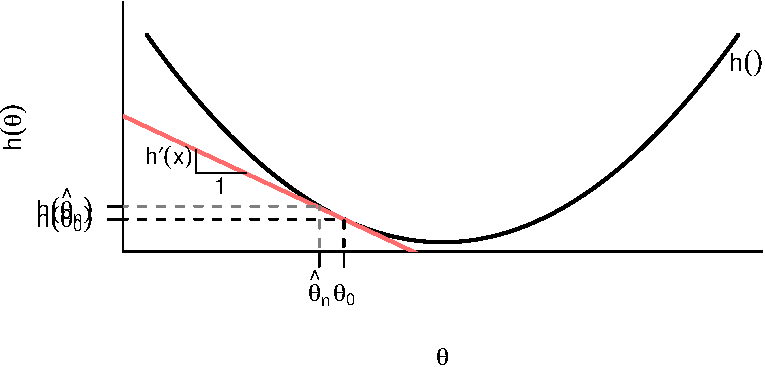
\includegraphics{asymptotics_files/figure-pdf/fig-delta-1.pdf}

}

\caption{\label{fig-delta}Linear approximation to nonlinear functions.}

\end{figure}%

\begin{example}[]\protect\hypertarget{exm-log}{}\label{exm-log}

Let's return to the iid sample \(X_1, \ldots, X_n\) with mean
\(\mu = \E[X_i]\) and variance \(\sigma^2 = \V[X_i]\). From the CLT, we
know that \(\sqrt{n}(\Xbar_n - \mu) \indist \N(0, \sigma^2)\). Suppose
that we want to estimate \(\log(\mu)\), so we use the plug-in estimator
\(\log(\Xbar_n)\) (assuming that \(X_i > 0\) for all \(i\) so that we
can take the log). What is the asymptotic distribution of this
estimator? This is a situation where \(\widehat{\theta}_n = \Xbar_n\)
and \(h(\mu) = \log(\mu)\). From basic calculus, we know that \[
h'(\mu) = \frac{\partial \log(\mu)}{\partial \mu} = \frac{1}{\mu},
\] so applying the delta method, we can determine that \[
\sqrt{n}\left(\log(\Xbar_n) - \log(\mu)\right) \indist \N\left(0,\frac{\sigma^2}{\mu^2} \right).
\]

\end{example}

\begin{example}[]\protect\hypertarget{exm-exp}{}\label{exm-exp}

What about estimating the \(\exp(\mu)\) with \(\exp(\Xbar_n)\)? Recall
that \[
h'(\mu) = \frac{\partial \exp(\mu)}{\partial \mu} = \exp(\mu)
\] so applying the delta method, we have \[
\sqrt{n}\left(\exp(\Xbar_n) - \exp(\mu)\right) \indist \N(0, \exp(2\mu)\sigma^2),
\] since \(\exp(\mu)^2 = \exp(2\mu)\).

\end{example}

Like all of the results in this chapter, there is a multivariate version
of the delta method that is incredibly useful in practical applications.
For example, suppose we want to combine two different estimators (or two
different estimated parameters) to estimate another quantity. We now let
\(\mb{h}(\mb{\theta}) = (h_1(\mb{\theta}), \ldots, h_m(\mb{\theta}))\)
map from \(\mathbb{R}^k \to \mathbb{R}^m\) and be continuously
differentiable (we make the function bold since it returns an
\(m\)-dimensional vector). It will help us to use more compact matrix
notation if we introduce a \(m \times k\) Jacobian matrix of all partial
derivatives \[
\mb{H}(\mb{\theta}) = \mb{\nabla}_{\mb{\theta}}\mb{h}(\mb{\theta}) = \begin{pmatrix}
  \frac{\partial h_1(\mb{\theta})}{\partial \theta_1} & \frac{\partial h_1(\mb{\theta})}{\partial \theta_2} & \cdots & \frac{\partial h_1(\mb{\theta})}{\partial \theta_k} \\
  \frac{\partial h_2(\mb{\theta})}{\partial \theta_1} & \frac{\partial h_2(\mb{\theta})}{\partial \theta_2} & \cdots & \frac{\partial h_2(\mb{\theta})}{\partial \theta_k} \\
  \vdots & \vdots & \ddots & \vdots \\
  \frac{\partial h_m(\mb{\theta})}{\partial \theta_1} & \frac{\partial h_m(\mb{\theta})}{\partial \theta_2} & \cdots & \frac{\partial h_m(\mb{\theta})}{\partial \theta_k} 
\end{pmatrix},
\] which we can use to generate the equivalent multivariate linear
approximation \[
\left(\mb{h}(\widehat{\mb{\theta}}_n) - \mb{h}(\mb{\theta}_0)\right) \approx \mb{H}(\mb{\theta}_0)'\left(\widehat{\mb{\theta}}_n - \mb{\theta}_0\right).
\] We can use this fact to derive the multivariate delta method.

\begin{theorem}[]\protect\hypertarget{thm-multivariate-delta}{}\label{thm-multivariate-delta}

Suppose that
\(\sqrt{n}\left(\widehat{\mb{\theta}}_n - \mb{\theta}_0 \right) \indist \N(0, \mb{\Sigma})\),
then for any function \(\mb{h}\) that is continuously differentiable in
a neighborhood of \(\mb{\theta}_0\), we have \[
\sqrt{n}\left(\mb{h}(\widehat{\mb{\theta}}_n) - \mb{h}(\mb{\theta}_0) \right) \indist \N(0, \mb{H}\mb{\Sigma}\mb{H}'), 
\] where \(\mb{H} = \mb{H}(\mb{\theta}_0)\).

\end{theorem}

This result follows from the approximation above plus rules about
variances of random vectors. Recall that for any compatible matrix of
constants, \(\mb{A}\), we have
\(\V[\mb{A}'\mb{Z}] = \mb{A}\V[\mb{Z}]\mb{A}'\). The matrix of constants
appears twice here, like the matrix version of the ``squaring the
constant'' rule for variance.

The delta method is handy for generating closed-form approximations for
asymptotic standard errors, but the math is often quite complex for even
simple estimators. It is usually more straightforward for applied
researchers to use computational tools such as the bootstrap to
approximate the needed standard errors. The bootstrap has the trade-off
of taking more computational time to implement compared to the delta
method, but it is more easily adaptable across different estimators and
domains.

\section{Summary}\label{summary-2}

In this chapter, we covered asymptotic analysis, which considers how
estimators behave as we feed them larger and larger samples. While we
never actually have infinite data, asymptotic results provide
approximations that work quite well in practice. A \textbf{consistent}
estimator converges in probability to a desired quantity of interest. We
saw several ways of establishing consistency, including the \textbf{Law
of Large Numbers} for the sample mean, which converges in probability to
the population mean. The \textbf{Central Limit Theorem} tells us that
the sample mean will be approximately normally distributed when we have
large, iid samples. We also saw how the \textbf{continuous mapping
theorem} and \textbf{Slutsky's theorem} allow us to determine asymptotic
results for a broad class of estimators. Knowing the asymptotic
normality of an estimator allows us to derive \textbf{confidence
intervals} that are valid in large samples. Finally, the \textbf{delta
method} is a general tool for finding the asymptotic distribution of an
estimator that is a function of another estimator with a known
asymptotic distribution.

In the next chapter, we will leverage these asymptotic results to
introduce another important tool for statistical inference: the
hypothesis test.

\chapter{Hypothesis tests}\label{sec-hypothesis-tests}

We have up to now discussed the properties of estimators that allow us
to characterize their distributions in finite and large samples. These
properties allow us to say, for example, that our estimated difference
in means is equal to a true average treatment effect on average across
repeated samples or that it will converge to the true value in large
samples. These properties, however, are properties of repeated samples.
Most researchers, on the other hand, will only have access to a single
sample. \textbf{Statistical inference} is the process of using a single
sample to learn about population parameters. As we will see, many common
techniques of statistical inference are intuitively closely connected.
One of the most ubiquitous in the social sciences is the hypothesis
test, a kind of statistical thought experiment.

\section{The Lady Tasting Tea}\label{the-lady-tasting-tea}

The story of the Lady Tasting Tea exemplifies the core ideas behind
hypothesis testing.\footnote{The analysis here largely comes from Senn
  (2012).} The story goes like this. R.A. Fisher, the early 20th-century
British polymath and statistical pioneer, had prepared tea for his
colleague, the algologist Muriel Bristol. Knowing that she preferred
milk in her tea, he poured milk into a tea cup and then poured the hot
tea into the milk and swirled it around. But Bristol rejected the cup,
stating that she preferred pouring the tea first, then the milk. Fisher
was skeptical of the idea that anyone could tell the difference between
a cup poured milk-first versus tea-first, and so he and another
colleague, William Roach, devised a test to see if Bristol could tell
the difference between the two preparation methods.

Fisher and Roach prepared 8 cups of tea, four with the milk poured first
and four with the tea poured first. Then they presented the cups to
Bristol in a random order (though she knew there were four of each
type), and she proceeded to identify all of the cups correctly. At first
glance, this seems like good evidence that she could tell the difference
between the two types of tea, but Fisher, being a natural skeptic,
raised the question, ``Could she have just been randomly guessing and
got lucky?'' This led Fisher to a \textbf{statistical thought
experiment}: what would the probability of identifying the correct cups
be \emph{if} she was guessing randomly?

To calculate the probability of Bristol identifying the four milk-first
cups correctly, note that ``randomly guessing'' would mean that she was
selecting a group of 4 cups to be labeled milk-first from the 8 cups
available. Using basic combinatorics, there are 70 ways to choose 4 cups
among 8, but only 1 of those arrangements would be correct. Thus, if
randomly guessing means choosing among those 70 options with equal
chance, then the probability of guessing the right set of cups is 1/70
or \(\approx 0.014\). The low probability implies that the hypothesis of
random guessing may be implausible.

The story of the Lady Tasting Tea encapsulates many of the core elements
of hypothesis testing. Hypothesis testing is about taking our observed
estimate (Bristol identifying all four cups correctly) and seeing how
likely that observed estimate would be under some assumption, or
hypothesis, about the data-generating process (Bristol was randomly
guessing). When the observed estimate is unlikely under the maintained
hypothesis, we might view this as evidence against that hypothesis.
Thus, hypothesis tests help us assess evidence for particular guesses
about the DGP.

\begin{tcolorbox}[enhanced jigsaw, toptitle=1mm, bottomrule=.15mm, leftrule=.75mm, rightrule=.15mm, breakable, colframe=quarto-callout-note-color-frame, title=\textcolor{quarto-callout-note-color}{\faInfo}\hspace{0.5em}{Notation alert}, colbacktitle=quarto-callout-note-color!10!white, titlerule=0mm, coltitle=black, left=2mm, colback=white, bottomtitle=1mm, opacitybacktitle=0.6, opacityback=0, toprule=.15mm, arc=.35mm]

For the rest of this chapter, we will introduce the concepts following
the notation in the past chapters. We will assume a random (iid) sample
of random variables \(X_1, \ldots, X_n\) from a distribution, \(F\).
We'll focus on estimating some parameter, \(\theta\), of this
distribution (like the mean, median, variance, etc.), and we will refer
to \(\Theta\) as the set of possible values of \(\theta\) or the
\textbf{parameter space}.

\end{tcolorbox}

\section{Hypotheses}\label{hypotheses}

In the context of hypothesis testing, hypotheses are simply statements
about the population distribution. In particular, we will make
statements that \(\theta = \theta_0\) where \(\theta_0 \in \Theta\) is
the hypothesized value of \(\theta\), a population parameter. Hypotheses
are ubiquitous in empirical work. Examples include:

\begin{itemize}
\tightlist
\item
  The population proportion of US citizens who identify as Democrats is
  0.33.
\item
  The population difference in average voter turnout between households
  who received get-out-the-vote mailers vs.~those who did not is 0.
\item
  The difference in the average incidence of human rights abuse in
  countries that signed a human rights treaty vs.~those countries that
  did not sign is 0.
\end{itemize}

Each of these is a statement about the true DGP. The latter two are
examples where the hypothesis is phrased as a possible non-difference,
which is very common. When \(\theta\) represents the difference in means
between two groups, then \(\theta = 0\) is the hypothesis of no actual
difference in population means or no treatment effect (if the causal
effect is identified).

The goal of hypothesis testing is to adjudicate between two
complementary hypotheses.

\begin{definition}[]\protect\hypertarget{def-null}{}\label{def-null}

The two hypotheses in a hypothesis test are called the \textbf{null
hypothesis} and the \textbf{alternative hypothesis}, denoted as \(H_0\)
and \(H_1\), respectively.

\end{definition}

These hypotheses are complementary, so if the null hypothesis is
\(H_0: \theta \in \Theta_0\), then the alternative hypothesis is
\(H_1: \theta \in \Theta_0^c\). The ``null'' in null hypothesis may seem
odd until you realize that most null hypotheses are that there is no
effect of some treatment or no difference in means. For example, suppose
that \(\theta\) is the difference in mean support for increasing legal
immigration between a treatment group that received a pro-immigrant
message with some facts about immigration and a control group that just
received the immigration facts. The usual null hypothesis would be no
difference in means or \(H_0: \theta = 0\), and the alternative would be
\(H_1: \theta \neq 0\). Substantively, the null hypothesis would posit
no average difference in the outcome -- in this case support for
increasing legal immigration -- between the two groups.

There are two common types of tests that differ in terms of the form of
their null and alternative hypotheses. A \textbf{two-sided test} is of
the form \[
H_0: \theta = \theta_0 \quad\text{versus}\quad H_1: \theta \neq \theta_0,
\] where the ``two-sided'' part refers to how the alternative contains
values of \(\theta\) above and below the null value \(\theta_0\).

A \textbf{one-sided test} is of the form \[
H_0: \theta \leq \theta_0 \quad\text{versus}\quad H_1: \theta > \theta_0,
\] or \[
H_0: \theta \geq \theta_0 \quad\text{versus}\quad H_1: \theta < \theta_0.
\] Where the ``one-sided'' part refers to how the alternative contains
values of \(\theta\) only above or below the null value. Two-sided tests
are much more common in the social sciences, mostly because we usually
want to know if there is any evidence, positive or negative, against the
presumption of no treatment effect or no relationship between two
variables. One-sided tests are best suited for situations with clear,
directional hypotheses that are ideally preregistered before collection
of the data. Preregistration of the direction of a one-sided test is
important because researchers changing the direction of the hypothesis
after seeing the data can inflate the strength of evidence against the
null. For this reason, one-sided tests outside of preregistered settings
should be used with extreme caution. That said, unfortunately, the math
of two-sided tests is also more complicated.

\section{The procedure of hypothesis
testing}\label{the-procedure-of-hypothesis-testing}

At the most basic level, a \textbf{hypothesis test} is a rule that
specifies values of the sample data for which we will decide to
\textbf{reject} the null hypothesis. Let \(\mathcal{X}_n\) be the range
of the sample---that is, all possible vectors \((x_1, \ldots, x_n)\)
that have a positive probability of occurring. A hypothesis test then
describes a region of this space, \(R \subset \mathcal{X}_n\), called
the \textbf{rejection region} where when \((X_1, \ldots, X_n) \in R\) we
will \textbf{reject} \(H_0\) and when the data is outside this region,
\((X_1, \ldots, X_n) \notin R\) we \textbf{retain}, \textbf{accept}, or
\textbf{fail to reject} the null hypothesis.\footnote{Different people
  and different textbooks describe what to do when we do not reject the
  null hypothesis differently. The terminology is not so important so
  long as you understand that rejecting the null does not mean the null
  is logically false and that ``accepting'' (or failing to reject) the
  null does not mean the null is logically true.}

How do we decide what the rejection region should be? Even though we
define the rejection region in terms of the \textbf{sample space},
\(\mathcal{X}_n\), working with the entire vector of data can be
unwieldy. We instead usually formulate the rejection region in terms of
a \textbf{test statistic}, \(T = T(X_1, \ldots, X_n)\), where the
rejection region becomes \[
R = \left\{(x_1, \ldots, x_n) : T(x_1, \ldots, x_n) > c\right\},
\] where \(c\) is called the \textbf{critical value}. This expression
says that the rejection region is the collection of possible data sets
that make the test statistic sufficiently large. Thus, the test
statistic is a function of the data that should get larger as the
observed data becomes incompatible with the null hypothesis. The
critical value (and thus the rejection region) demarcates when the
divergence between the observed data and the null hypothesis is large
enough to allow us to reject the null hypothesis. Note that the test
statistic is a random variable and has a distribution. We will exploit
this later to better understand the different properties of a hypothesis
test.

Consider a simple one-sided test where you feel a bit ill and try to
determine if you have a normal body temperature of 98.7 degrees
Fahrenheit or if you have a fever. In this case, the thermometer reading
is the test statistic since a larger reading are less consistent with a
normal body temperature. Thermometers, however, are imperfect and noisy
tools, so the reading might differ from 98.7 even if one's temperature
is normal. Thus, we can use a rejection region such as readings over
100.5 degrees to determine when to reject the null hypothesis of a
normal body temperature.

\begin{example}[]\protect\hypertarget{exm-biden}{}\label{exm-biden}

Suppose that \((X_1, \ldots, X_n)\) represents a sample of US citizens
where \(X_i = 1\) indicates support for the current US president and
\(X_i = 0\) means opposition (no support). A good and reasonable null
hypothesis is that the president does not have the support of a majority
of American citizens. Let \(\mu = \E[X_i] = \P(X_i = 1)\). Then, a
one-sided test would compare the two hypotheses: \[ 
H_0: \mu \leq 0.5 \quad\text{versus}\quad H_1: \mu > 0.5.
\] In this case, we might use the sample mean as the test statistic, so
that \(T(X_1, \ldots, X_n) = \Xbar_n\), and we have to find some
threshold above 0.5 such that we would reject the null, \[ 
R = \left\{(x_1, \ldots, x_n): \Xbar_n > c\right\}.
\] In words, we are asking how much support should we see for the
current president before we reject the notion that he or she lacks
majority support? Below we will select the critical value, \(c\), to
have beneficial statistical properties.

\end{example}

The structure of a reject region will depend on whether a test is one-
or two-sided. This is an important point of difference between the two
test types that we will raise again below. One-sided tests will take the
form \(T > c\), whereas two-sided tests will take the form \(|T| > c\)
since we want to count deviations from either side of the null
hypothesis as evidence against that null.

\section{Testing errors}\label{testing-errors}

Hypothesis tests end with a decision to reject the null hypothesis or
not, but this might be an incorrect decision. In particular, there are
two ways to make errors and two ways to be correct in this setting, as
shown in Table~\ref{tbl-errors}. The labels are confusing, but remember
that \textbf{Type I errors} (said ``type one'') are labeled so because
they are the worst of the two types of errors. Type I errors occur when
we reject a null when the null is in fact true. For example, if we have
a null hypothesis of no treatment effect between a treatment and control
condition, and we reject that null hypothesis (and conclude
substantively that there is some sort of a treatment effect), then we
would be committing a Type I error if in fact the null was true -- that
is, there is no real treatment effect but we concluded there was one.
Type I errors are what we see in the replication crisis: lots of
``significant'' effects that turn out later to be null.

\textbf{Type II errors} (said ``type two'') are generally considered
less problematic. For such errors, There is a true relationship, but we
cannot detect it with our test. That is, we do not reject a null that is
false. For example, if we have a null hypothesis of no treatment effect
between a treatment and control condition, we would be committing a Type
II error if in fact there was a difference in the treatment and control
but we concluded there wasn't (we failed to reject the null hypothesis
of no difference).

\begin{longtable}[]{@{}lll@{}}
\caption{Typology of testing errors}\label{tbl-errors}\tabularnewline
\toprule\noalign{}
& \(H_0\) True & \(H_0\) False \\
\midrule\noalign{}
\endfirsthead
\toprule\noalign{}
& \(H_0\) True & \(H_0\) False \\
\midrule\noalign{}
\endhead
\bottomrule\noalign{}
\endlastfoot
Retain \(H_0\) & Awesome & Type II error \\
Reject \(H_0\) & Type I error & Great \\
\end{longtable}

Ideally, we would minimize the chances of making either a Type I or Type
II error. Unfortunately, because the test statistic is a random
variable, we cannot remove the probability of an error altogether.
Instead, we will derive tests with some guaranteed performance to
minimize the probability of Type I error, usually the more objectionable
type of error. To derive this, we can define the \textbf{power function}
of a test, \[ 
\pi(\theta) = \P\left( \text{Reject } H_0 \mid \theta \right) = \P\left( T \in R \mid \theta \right),
\] which is the probability of rejection as a function of the parameter
of interest, \(\theta\). The power function tells us, for example, how
likely we are to reject the null hypothesis of no treatment effect (no
difference) as we vary the actual size of the treatment effect (which in
this case is \(\theta\)).

We can define the probability of Type I error from the power function.

\begin{definition}[]\protect\hypertarget{def-size}{}\label{def-size}

The \textbf{size} of a hypothesis test with the null hypothesis
\(H_0: \theta = \theta_0\) is \[ 
\pi(\theta_0) = \P\left( \text{Reject } H_0 \mid \theta_0 \right).
\]

\end{definition}

You can think of the size of a test as the rate of false positives (or
false discoveries) produced by the test. Figure~\ref{fig-size-power}
shows an example of rejection regions, size, and power for a one-sided
test. In the left panel, we have the distribution of the test statistic
under the null, with \(H_0: \theta = \theta_0\), and the rejection
region is defined by values \(T > c\). We refer to the distribution of
the test statistic under the null hypothesis as the \textbf{null
distribution} or the \textbf{reference distribution}. The shaded gray
region is the probability of rejection under this null hypothesis, or
the size of the test. Sometimes, we will get extreme samples by random
chance, even under the null, leading to false discoveries.\footnote{Eagle-eyed
  readers will notice that the null tested here is a point, while we
  previously defined the null in a one-sided test as a region
  \(H_0: \theta \leq \theta_0\). Technically, the size of the test will
  vary based on which of these nulls we choose. In this example, notice
  that any null to the left of \(\theta_0\) will result in a lower size.
  And so, the null at the boundary, \(\theta_0\), will maximize the size
  of the test, making it the most ``conservative'' null to investigate.
  Technically, we should define the size of a test as
  \(\alpha = \sup_{\theta \in \Theta_0} \pi(\theta)\).}

In the right panel, we overlay the distribution of the test statistic
under one particular alternative, \(\theta = \theta_1 > \theta_0\). The
red-shaded region is the probability of rejecting the null when this
alternative is true for the power---it is the probability of correctly
rejecting the null when it is false. Intuitively, we can see that
alternatives that produce test statistics closer to the rejection region
will have higher power. This makes sense: detecting big deviations from
the null should be easier than detecting minor ones.

\begin{figure}[th]

\centering{

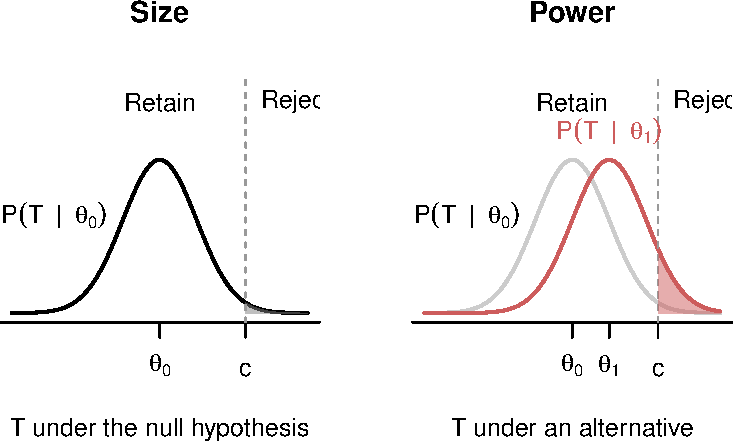
\includegraphics{hypothesis_tests_files/figure-pdf/fig-size-power-1.pdf}

}

\caption{\label{fig-size-power}Size of a test and power against an
alternative.}

\end{figure}%

Figure~\ref{fig-size-power} also hints at a tradeoff between size and
power. Notice that we could make the size smaller (lower the false
positive rate) by increasing the critical value to \(c' > c\). This
would make the probability of being in the rejection region smaller,
\(\P(T > c' \mid \theta_0) < \P(T > c \mid \theta_0)\), leading to a
lower-sized test. Unfortunately, it would also reduce power in the right
panel since the probability of being in the rejection region will be
lower under any alternative,
\(\P(T > c' \mid \theta_1) < \P(T > c \mid \theta_1)\). This means we
usually cannot simultaneously reduce both types of errors.

\section{Determining the rejection
region}\label{determining-the-rejection-region}

If we cannot simultaneously optimize a test's size and power, how should
we determine where the rejection region is? That is, how should we
decide what empirical evidence will be strong enough for us to reject
the null? The standard approach is to control the size of a test (that
is, control the rate of false positives) and try to maximize the power
of the test subject to that constraint. So we say, ``I'm willing to
accept at most X\%'' of findings will be false positives and do whatever
we can to maximize power subject to that constraint.

\begin{definition}[]\protect\hypertarget{def-level}{}\label{def-level}

A test has \textbf{significance level} \(\alpha\) if its size is less
than or equal to \(\alpha\), or \(\pi(\theta_0) \leq \alpha\).

\end{definition}

A test with a significance level of \(\alpha = 0.05\) will have a false
positive/Type I error rate no larger than 0.05. This level is widespread
in the social sciences, though you also will see \(\alpha = 0.01\) or
\(\alpha = 0.1\). Frequentists justify this by saying this means that
with \(\alpha = 0.05\), there will only be at most 5\% of studies that
will produce false discoveries.

Our task is to construct the rejection region so that the \textbf{null
distribution} of the test statistic
\(G_0(t) = \P(T \leq t \mid \theta_0)\) has less than \(\alpha\)
probability in that region. One-sided tests like in
Figure~\ref{fig-size-power} are the easiest to show, even though we
warned you not to use them. We want to choose \(c\) that puts no more
than \(\alpha\) probability in the tail, or \[ 
\P(T > c \mid \theta_0) = 1 - G_0(c) \leq \alpha.
\] Remember that the smaller the value of \(c\) we can use will maximize
power, which implies that the critical value for the maximum power while
maintaining the significance level is when \(1 - G_0(c) = \alpha\). We
can use the \textbf{quantile function} of the null distribution to find
the exact value of \(c\) we need, \[
c = G^{-1}_0(1 - \alpha),
\] which substantively translates to say, ``the value at which
\(1-\alpha\) of the null distribution is below.''

The determination of the rejection region follows the same principles
for two-sided tests, but it is more complicated because we reject when
the magnitude of the test statistic is large, \(|T| > c\).
Figure~\ref{fig-two-sided} shows that basic setup. Notice that because
there are two (disjoint) regions, one on the left and one on the right,
we can write the size (false positive rate) as \[ 
\pi(\theta_0) = G_0(-c) + 1 - G_0(c).
\] In most cases, the null distribution for such a test will be
symmetric around 0 (usually asymptotically standard normal, actually),
which means that \(G_0(-c) = 1 - G_0(c)\). This in turn implies that the
size is \[ 
\pi(\theta_0) = 2(1 - G_0(c)).
\] Solving for the critical value that would make this \(\alpha\) gives
\[ 
c = G^{-1}_0(1 - \alpha/2).
\] Again, this formula can seem dense, but remember what you are doing:
finding the value that puts \(\alpha/2\) of the probability of the null
distribution in each tail.

\begin{figure}[th]

\centering{

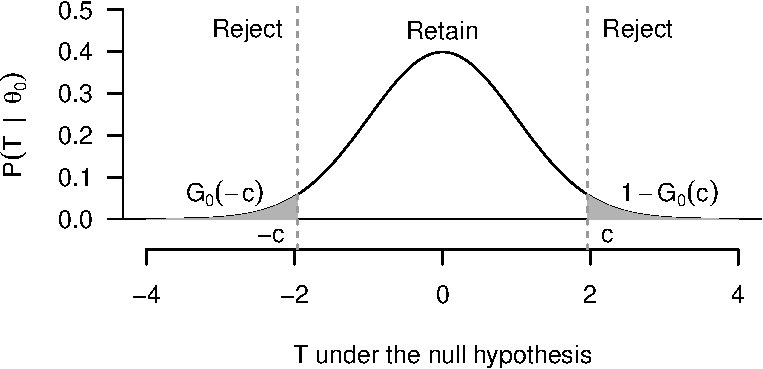
\includegraphics{hypothesis_tests_files/figure-pdf/fig-two-sided-1.pdf}

}

\caption{\label{fig-two-sided}Rejection regions for a two-sided test.}

\end{figure}%

\section{Hypothesis tests of the sample
mean}\label{hypothesis-tests-of-the-sample-mean}

Consider the following extended example about hypothesis testing of a
sample mean, sometimes called a \textbf{one-sample test} since we are
usually using just one sample statistic (the sample mean in this case)
and comparing that to some sort of natural conceptual benchmark. Let's
say \(X_i\) represents feeling thermometer scores about ``liberals'' as
a group on a scale of 0 to 100, with values closer to 0 indicating
cooler feelings about liberals and values closer to 100 indicating
warmer feelings about liberals. (This is similar to many survey items on
nationally representative surveys, such as the ANES in the U.S.) We want
to know if the population average differs from a value of 50, which is a
good benchmark that would indicate roughly neutral feelings toward
liberals. We can write this two-sided test as \[
H_0: \mu = 50 \quad\text{versus}\quad H_1: \mu \neq 50,
\] where \(\mu = \E[X_i]\). The standard test statistic for this type of
test is the so-called \textbf{t-statistic}, \[ 
T = \frac{\left( \Xbar_n - \mu_0 \right)}{\sqrt{s^2 / n}} =\frac{\left( \Xbar_n - 50 \right)}{\sqrt{s^2 / n}},
\] where \(\mu_0\) is the null value of interest and \(s^2\) is the
sample variance. If the null hypothesis is true, then by the CLT, we
know that the t-statistic is asymptotically normal,
\(T \indist \N(0, 1)\). Thus, we can approximate the null distribution
with the standard normal.

\begin{tcolorbox}[enhanced jigsaw, toptitle=1mm, bottomrule=.15mm, leftrule=.75mm, rightrule=.15mm, breakable, colframe=quarto-callout-warning-color-frame, title=\textcolor{quarto-callout-warning-color}{\faExclamationTriangle}\hspace{0.5em}{Warning}, colbacktitle=quarto-callout-warning-color!10!white, titlerule=0mm, coltitle=black, left=2mm, colback=white, bottomtitle=1mm, opacitybacktitle=0.6, opacityback=0, toprule=.15mm, arc=.35mm]

The names of the various tests can be quite confusing because they are
so similar. Earlier, we discussed one-sided versus two-sided tests,
which differed in what alternative hypotheses were being considered.
One-sample and two-sample tests, on the other hand, describe how many
group means we are comparing. In a one-sample test, we compare one
population mean to a fixed number. For two-sample tests (described in
more detail below), we are usually making null hypotheses about the
different between two population means.

\end{tcolorbox}

Let's create a two-sided test with level \(\alpha = 0.05\), our
tolerance for Type I error. Then we need to find the rejection region
that puts \(0.05\) probability in the tails of the null distribution,
which we just saw was \(\N(0,1)\). Let \(\Phi()\) be the CDF for the
standard normal and let \(\Phi^{-1}()\) be the quantile function for the
standard normal. Drawing on what we developed above, you can find the
value \(c\) so that \(\P(|T| > c \mid \mu_0)\) is 0.05 with \[
c = \Phi^{-1}(1 - 0.05/2) \approx 1.96,
\] This means that a test where we reject when \(|T| > 1.96\) would have
a level of 0.05 asymptotically.

\section{The Wald test}\label{the-wald-test}

We can generalize the hypothesis test for the sample mean to estimators
more broadly. Let \(\widehat{\theta}_n\) be an estimator for some
parameter \(\theta\) and let
\(\widehat{\textsf{se}}[\widehat{\theta}_n]\) be a consistent estimate
of the standard error of the estimator,
\(\textsf{se}[\widehat{\theta}_n] = \sqrt{\V[\widehat{\theta}_n]}\). We
consider the two-sided test \[
H_0: \theta = \theta_0 \quad\text{versus}\quad H_1: \theta \neq \theta_0.
\]

In many cases, our estimators will be asymptotically normal by a version
of the CLT so that under the null hypothesis, we have \[ 
T = \frac{\widehat{\theta}_n - \theta_0}{\widehat{\textsf{se}}[\widehat{\theta}_n]} \indist \N(0, 1). 
\] The \textbf{Wald test} rejects \(H_0\) when \(|T| > z_{\alpha/2}\),
with \(z_{\alpha/2}\) that puts \(\alpha/2\) in the upper tail of the
standard normal. That is, if \(Z \sim \N(0, 1)\), then \(z_{\alpha/2}\)
satisfies \(\P(Z \geq z_{\alpha/2}) = \alpha/2\).

\begin{tcolorbox}[enhanced jigsaw, toptitle=1mm, bottomrule=.15mm, leftrule=.75mm, rightrule=.15mm, breakable, colframe=quarto-callout-note-color-frame, title=\textcolor{quarto-callout-note-color}{\faInfo}\hspace{0.5em}{Note}, colbacktitle=quarto-callout-note-color!10!white, titlerule=0mm, coltitle=black, left=2mm, colback=white, bottomtitle=1mm, opacitybacktitle=0.6, opacityback=0, toprule=.15mm, arc=.35mm]

In R, you can find the \(z_{\alpha/2}\) values easily with the
\texttt{qnorm()} function:

\begin{Shaded}
\begin{Highlighting}[]
\FunctionTok{qnorm}\NormalTok{(}\FloatTok{0.05} \SpecialCharTok{/} \DecValTok{2}\NormalTok{, }\AttributeTok{lower.tail =} \ConstantTok{FALSE}\NormalTok{)}
\end{Highlighting}
\end{Shaded}

\begin{verbatim}
[1] 1.959964
\end{verbatim}

\end{tcolorbox}

\begin{theorem}[]\protect\hypertarget{thm-wald}{}\label{thm-wald}

Asymptotically, the Wald test has size \(\alpha\) such that \[ 
\P(|T| > z_{\alpha/2} \mid \theta_0) \to \alpha.
\]

\end{theorem}

This result is very general, and it means that many, many hypothesis
tests based on estimators will have the same form. The main difference
across estimators will be how we calculate the estimated standard error.

\begin{example}[Difference in
proportions]\protect\hypertarget{exm-two-props}{}\label{exm-two-props}

Get-out-the-vote (GOTV) experiments are common in political science. A
typical GOTV design might randomly assign a group of citizens to receive
mailers encouraging them to vote, whereas a control group receives no
message. We will define the turnout variables in the treatment group,
\(Y_{1}, Y_{2}, \ldots, Y_{n_t}\), as iid draws from a Bernoulli
distribution with success \(p_t\), which represents the population
turnout rate in the treated group treated. The outcomes in the control
group, \(X_{1}, X_{2}, \ldots, X_{n_c}\), are iid draws from another
Bernoulli distribution with success \(p_c\), which represents the
population turnout rate among citizens not receiving a mailer.

Our goal is to learn about the effect of this treatment on whether a
citizen votes, \(\tau = p_t - p_c\), and we will use the sample
difference in means/proportions as our estimator,
\(\widehat{\tau} = \Ybar - \Xbar\). To perform a Wald test, we need to
either know or estimate the standard error of this estimator. Notice
that because these are independent samples, the variance is \[ 
\V[\widehat{\tau}_n] = \V[\Ybar - \Xbar] = \V[\Ybar] + \V[\Xbar] = \frac{p_t(1-p_t)}{n_t} + \frac{p_c(1-p_c)}{n_c},
\] where the third equality comes from the fact that the underlying
outcome variables \(Y_i\) and \(X_j\) are binary. Obviously, we do not
know the true population proportions \(p_t\) and \(p_c\) (that's why
we're doing the test!), but we can estimate the standard error by
replacing them with their estimates \[ 
\widehat{\textsf{se}}[\widehat{\tau}] = \sqrt{\frac{\Ybar(1 -\Ybar)}{n_t} + \frac{\Xbar(1-\Xbar)}{n_c}}.
\]

The typical null hypothesis test in this \textbf{two-sample test} is
``no treatment effect'' vs.~``some treatment effect'': \[
H_0: \tau = p_t - p_c = 0 \quad\text{versus}\quad H_1: \tau \neq 0,
\] which gives the following test statistic for the Wald test \[
T = \frac{\Ybar - \Xbar}{\sqrt{\frac{\Ybar(1 -\Ybar)}{n_t} + \frac{\Xbar(1-\Xbar)}{n_c}}}. 
\] If we wanted a test with level \(\alpha = 0.01\), we would reject the
null when \(|T| > 2.58\) since

\begin{Shaded}
\begin{Highlighting}[]
\FunctionTok{qnorm}\NormalTok{(}\FloatTok{0.01}\SpecialCharTok{/}\DecValTok{2}\NormalTok{, }\AttributeTok{lower.tail =} \ConstantTok{FALSE}\NormalTok{)}
\end{Highlighting}
\end{Shaded}

\begin{verbatim}
[1] 2.575829
\end{verbatim}

\end{example}

\begin{example}[Difference in
means]\protect\hypertarget{exm-diff-in-means}{}\label{exm-diff-in-means}

Consider a similar example with randomly assigned treatment and control
groups, but instead the treatment is now an appeal for financial
donations to a political campaign and the outcomes are continuous
measures of how much money a person has donated. The treatment data
\(Y_1, \ldots, Y_{n_t}\) are iid draws from a population with mean
\(\mu_t = \E[Y_i]\) and population variance \(\sigma^2_t = \V[Y_i]\).
The control data \(X_1, \ldots, X_{n_c}\) are iid draws (independent of
the \(Y_i\)) from a population with mean \(\mu_c = \E[X_i]\) and
population variance \(\sigma^2_c = \V[X_i]\). The parameter of interest
is similar to before: the population difference in means,
\(\tau = \mu_t - \mu_c\). We will form the usual hypothesis test of \[ 
H_0: \tau = \mu_t - \mu_c = 0 \quad\text{versus}\quad H_1: \tau \neq 0.
\]

The only difference between this setting and the
difference-in-proportions setting is that the standard error here is
different because we cannot rely on binary outcomes. Instead, we'll use
our knowledge of the sampling variance of the sample means and
independence between the samples to derive \[
\V[\widehat{\tau}] = \V[\Ybar] + \V[\Xbar] = \frac{\sigma^2_t}{n_t} + \frac{\sigma^2_c}{n_c},
\] where we can come up with an estimate of the unknown population
variance with sample variances \[
\widehat{\se}[\widehat{\tau}] = \sqrt{\frac{s^2_t}{n_t} + \frac{s^2_c}{n_c}}.
\] We can use this estimator to derive the Wald test statistic of \[ 
T = \frac{\widehat{\tau} - 0}{\widehat{\se}[\widehat{\tau}]} = \frac{\Ybar - \Xbar}{\sqrt{\frac{s^2_t}{n_t} + \frac{s^2_c}{n_c}}},
\] and if we want an asymptotic level of 0.05, we can reject when
\(|T| > 1.96\).

\end{example}

\section{p-values}\label{p-values}

The hypothesis testing framework focuses on making a decision -- to
reject the null hypothesis or not -- in the face of uncertainty. You
choose a level of wrongness you are comfortable with (rate of false
positives, or \(\alpha\)) and then decide null vs.~alternative based
firmly on the rejection region.

That said, note that we are discarding, somewhat artificially,
information on how far the observed data is from the null hypothesis. We
would ``accept'' the null if \(T = 1.95\) in the last example but would
reject it if \(T = 1.97\), even though these are very similar. Simply
reporting the reject/retain decision also fails to give us a sense of
possible other levels at which we might have rejected the null. Again,
this makes sense if we need to make a single decision: other tests don't
matter because we carefully considered our \(\alpha\) level test. But in
the lower-stakes world of the academic social sciences, we can afford to
be more informative.

One alternative to reporting the reject/retain decision is to report a
\textbf{p-value}.

\begin{definition}[]\protect\hypertarget{def-p-value}{}\label{def-p-value}

The \textbf{p-value} of a test is the probability of observing a test
statistic at least as extreme as the observed test statistic in the
direction of the alternative hypothesis.

\end{definition}

The line ``in the direction of the alternative hypothesis'' deals with
the unfortunate headache of one-sided versus two-sided tests. For a
one-sided test where larger values of \(T\) correspond to more evidence
for \(H_1\), the p-value is \[
\P(T(X_1,\ldots,X_n) > T \mid \theta_0) = 1 - G_0(T),
\] whereas for a (symmetric) two-sided test, we have \[ 
\P(|T(X_1, \ldots, X_n)| > |T| \mid \theta_0) = 2(1 - G_0(|T|)).
\]

In either case, the interpretation of the p-value is the same. It is the
smallest size \(\alpha\) at which a test would reject the null
hypothesis. Presenting a p-value allows the reader to determine their
own \(\alpha\) level and determine quickly if the evidence would warrant
rejecting \(H_0\) in that case. Thus, the p-value is a more
\textbf{continuous} measure of divergence between the observed data and
the null hypothesis. Lower values indicate more divergence because the
observed result is less likely under the null.

Much of the controversy surrounding p-values focuses on arbitrary
p-value cutoffs for determining statistical significance and sometimes
publication decisions. These problems are not the fault of p-values but,
rather, the hyperfixation on the reject/retain decision for arbitrary
test levels like \(\alpha = 0.05\). It might be best to view p-values as
a transformation of the test statistic onto a common scale between 0 and
1.

\begin{tcolorbox}[enhanced jigsaw, toptitle=1mm, bottomrule=.15mm, leftrule=.75mm, rightrule=.15mm, breakable, colframe=quarto-callout-warning-color-frame, title=\textcolor{quarto-callout-warning-color}{\faExclamationTriangle}\hspace{0.5em}{Warning}, colbacktitle=quarto-callout-warning-color!10!white, titlerule=0mm, coltitle=black, left=2mm, colback=white, bottomtitle=1mm, opacitybacktitle=0.6, opacityback=0, toprule=.15mm, arc=.35mm]

People use many statistical shibboleths to purportedly identify people
who don't understand statistics, and these criticisms sometimes hinge on
seemingly subtle differences in interpretation that are easy to miss. If
you have intuitively mastered the core concepts, however, avoiding these
common pitfalls will be much easier.

The shibboleth with p-values is that sometimes people interpret them as
``the probability that the null hypothesis is true.'' But this doesn't
make sense from our definition because the p-value \emph{conditions} on
the null hypothesis---it cannot tell us anything about the probability
of the null hypothesis being true. A more useful metaphor is that
hypothesis tests are statistical thought experiments and that p-values
answer the question: how likely would my data be if the null were true?

\end{tcolorbox}

\section{Power analysis}\label{power-analysis}

Imagine you have spent a large amount of your research budget on a big
experiment that tests a new and exciting theory, but the results come
back, and\ldots{} you fail to reject the null of no treatment effect.
This can happen under two possible states of the world: (1) the null is
true, and you correctly failed to reject it, or (2) the null is false
but the test had insufficient power to detect the true effect (that is,
to allow you to reject the null). Because this is unwanted uncertainty
after the fact, it is common for researchers to conduct \textbf{power
analyses} before collecting data. These analyses forecast the necessary
sample size to ensure you can reject the null under a hypothesized
effect size. These hypothesized effect sizes are vital to this exercise
and often come from prior studies or substantive knowledge about the
domain.

Generally power analyses involve calculating the power function
\(\pi(\theta) = \P(T(X_1, \ldots, X_n) \in R \mid \theta)\) for
different values of \(\theta\). It might also involve sample size
calculations for a particular alternative, \(\theta_1\), the
hypothesized treatment effect. In that case, we try to find the sample
size \(n\) to make the power \(\pi(\theta_1)\) as close to a particular
value (often 0.8) as possible. For simpler one-sided tests, solving for
the sample size is straightforward. For more general situations or
two-sided tests, however, we typically need numerical or
simulation-based approaches to find the optimal sample size.

With Wald tests, we can characterize the power function quite easily,
even if the test does not allow us to back out sample size calculations
easily.

\begin{theorem}[]\protect\hypertarget{thm-power}{}\label{thm-power}

For a Wald test with an asymptotically normal estimator, the power
function for a particular alternative \(\theta_1 \neq \theta_0\) is \[ 
\pi(\theta_1) = 1 - \Phi\left( \frac{\theta_0 - \theta_1}{\widehat{\se}[\widehat{\theta}_n]} + z_{\alpha/2} \right) + \Phi\left( \frac{\theta_0 - \theta_1}{\widehat{\se}[\widehat{\theta}_n]}-z_{\alpha/2} \right).
\]

\end{theorem}

\section{Exact tests under normal
data}\label{exact-tests-under-normal-data}

The Wald test above relies on large-sample approximations but these may
not be valid in finate samples. Can we get \textbf{exact} inferences at
any sample size? Yes, if we make stronger assumptions about the data. In
particular, assume a \textbf{parametric model} for the data where
\(X_1,\ldots,X_n\) are iid samples from \(N(\mu,\sigma^2)\). Under a
null hypothesis of \(H_0: \mu = \mu_0\), we can show that \[ 
T_n = \frac{\Xbar_n - \mu_0}{s_n/\sqrt{n}} \sim t_{n-1},
\] where \(t_{n-1}\) is the \textbf{Student's t-distribution} with
\(n-1\) degrees of freedom. This result implies the null distribution is
\(t\), so we use quantiles of \(t\) for critical values. For a one-sided
test, \(c = G^{-1}_0(1 - \alpha)\), but now \(G_0\) is \(t\) with
\(n-1\) df and so we use \texttt{qt()} instead of \texttt{qnorm()} to
calculate these critical values.

The critical values for the \(t\) distribution are always larger than
the normal because the t distribution has fatter tails, as shown in
Figure~\ref{fig-shape-of-t}. As \(n\to\infty\), however, the \(t\)
converges to the standard normal, and so it is asymptotically equivalent
to the Wald test but slightly more conservative in finite samples. Most
software packages calculate p-values and rejection regions based on the
\(t\) to exploit this conservativeness.

\begin{figure}[th]

\centering{

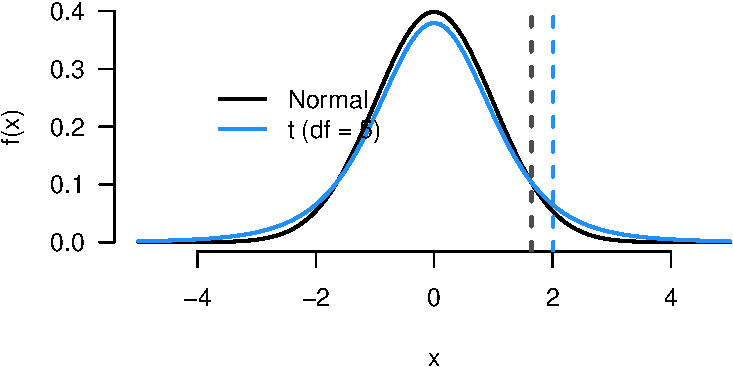
\includegraphics{hypothesis_tests_files/figure-pdf/fig-shape-of-t-1.pdf}

}

\caption{\label{fig-shape-of-t}Normal versus t distribution.}

\end{figure}%

\section{Confidence intervals and hypothesis
tests}\label{confidence-intervals-and-hypothesis-tests}

At first glance, we may seem sloppy in using \(\alpha\) in deriving a
\(1 - \alpha\) confidence interval in the last chapter and an
\(\alpha\)-level test in this chapter. In reality, we were foreshadowing
the deep connection between confidence intervals and hypothesis tests:
every \(1-\alpha\) confidence interval contains all null hypotheses that
we \textbf{would not reject} with an \(\alpha\)-level test.

This connection is easiest to see with an asymptotically normal
estimator, \(\widehat{\theta}_n\). Consider the hypothesis test of \[ 
H_0: \theta = \theta_0 \quad \text{vs.}\quad H_1: \theta \neq \theta_0,
\] using the test statistic, \[ 
T = \frac{\widehat{\theta}_{n} - \theta_{0}}{\widehat{\se}[\widehat{\theta}_{n}]}. 
\] As we discussed earlier, an \(\alpha = 0.05\) test would reject this
null when \(|T| > 1.96\), or when \[ 
|\widehat{\theta}_{n} - \theta_{0}| > 1.96 \widehat{\se}[\widehat{\theta}_{n}]. 
\] Notice that will be true when \[ 
\theta_{0} < \widehat{\theta}_{n} - 1.96\widehat{\se}[\widehat{\theta}_{n}]\quad \text{ or }\quad \widehat{\theta}_{n} + 1.96\widehat{\se}[\widehat{\theta}_{n}] < \theta_{0}
\] or, equivalently, that null hypothesis is outside of the 95\%
confidence interval,
\[\theta_0 \notin \left[\widehat{\theta}_{n} - 1.96\widehat{\se}[\widehat{\theta}_{n}], \widehat{\theta}_{n} + 1.96\widehat{\se}[\widehat{\theta}_{n}]\right].\]

Our choice of the null hypothesis was arbitrary, which means that any
null hypothesis outside the 95\% confidence interval would be rejected
by a \(\alpha = 0.05\) level test. And any null hypothesis inside the
confidence interval is a null hypothesis that we would not reject.

This relationship holds more broadly. Any \(1-\alpha\) confidence
interval contains all possible parameter values that would not be
rejected as the null hypothesis of an \(\alpha\)-level hypothesis test.
This connection can be handy for two reasons:

\begin{enumerate}
\def\labelenumi{\arabic{enumi}.}
\tightlist
\item
  We can quickly determine if we would reject a null hypothesis at some
  level by inspecting if it falls in a confidence interval. For example,
  quickly looking to see whether 0 is included in the confidence
  interval is a fast and easy check on whether a null hypothesis of no
  treatment effect is or is not rejected -- if it is included, the null
  cannot be rejected.
\item
  In some situations, determining a confidence interval might be
  difficult, but performing a hypothesis test is straightforward. Then,
  we can find the rejection region for the test and determine which null
  hypotheses would not be rejected at level \(\alpha\) to formulate the
  \(1-\alpha\) confidence interval. We call this process
  \textbf{inverting a test}. A critical application of this method is
  for formulating confidence intervals for treatment effects based on
  randomization inference in the finite population analysis of
  experiments.
\end{enumerate}

\section{Summary}\label{summary-3}

In this chapter, we covered the basics of hypothesis tests, which are a
type of statistical thought experiment. We assume that we know the true
state of the world and determine how unlikely our observed data would be
in that world. We described different types of tests (one-sided versus
two-sided), introduced the properties of tests (size and power), and
showed how to determine the rejection region of a test. We also
described the Wald test, a general test that can be used in a wide
variety of settings. P-values are a continuous measure of divergence
between the observed data and the null hypothesis. Power analyses allow
researchers to forecast how large of a sample they will need to detect
different effect sizes with sufficient statistical power. Finally,
confidence intervals and hypothesis tests are deeply connected since
confidence intervals will contain all null hypotheses that cannot be
rejected at a certain \(\alpha\).

We have now covered the basic tools of statistical inference at a high
level and have shown how to apply them to simple estimators like the
sample mean or the sample difference in means. In Part II of this book,
we turn to applying many of these ideas to the predominant estimator in
the quantitative social sciences---ordinary least squares.

\part{Regression}

\chapter{Linear regression}\label{sec-regression}

Regression is simply a set of tools for evaluating the relationship
between an \textbf{outcome variable}, \(Y_i\), and a set of
\textbf{covariates}, \(\X_i\). In particular, these tools show how the
conditional mean of \(Y_i\) varies as a function of \(\X_i\). For
example, we may want to know how wait times at voting precincts vary as
a function of various socioeconomic features of the precinct, like
income and racial composition. We can accomplish this by estimating the
\textbf{regression function} or \textbf{conditional expectation
function} (CEF) of the outcome given the covariates, \[
\mu(\bfx) = \E[Y_i \mid \X_i = \bfx].
\] Why are estimation and inference for this regression function
special? Why can't we just use the approaches we have seen for the mean,
variance, covariance, and so on? The fundamental problem with the CEF is
that there may be many values \(\bfx\) that can occur and many different
conditional expectations that we will need to estimate. If any variable
in \(\X_i\) is continuous, we must estimate an infinite number of
possible values of \(\mu(\bfx)\), and this worsens as we add covariates
to \(\X_i\). Because of that, we refer to this problem as the
\textbf{curse of dimensionality}. How can we resolve this with our
measly finite data?

In this chapter, we will explore two ways of ``solving'' the curse of
dimensionality: (1) assuming it away, and (2) changing the quantity of
interest to something easier to estimate.

Regression is so ubiquitous across many scientific fields that it has
generated a lot of acquired notational baggage. In particular, the
labels of the \(Y_i\) and \(\X_i\) vary greatly:

\begin{itemize}
\tightlist
\item
  The outcome can also be called: the response variable, the dependent
  variable, the labels (in machine learning), the left-hand side
  variable, or the regressand
\item
  The covariates are also called: the explanatory variables, the
  independent variables, the predictors, the right-hand side variables,
  the regressors, inputs, or features
\end{itemize}

\section{Why do we need models?}\label{why-do-we-need-models}

At first glance, the connection between the CEF and parametric models
might be hazy. For example, imagine we are interested in estimating the
average wait times at a voting precinct (\(Y_i\)) for Black voters
(\(X_i = 1\)) versus non-Black voters (\(X_i=0\)). In that case, there
are two parameters to estimate, \[
\mu(1) = \E[Y_i \mid X_i = 1] \quad \text{and}\quad \mu(0) = \E[Y_i \mid X_i = 0],
\] which we could estimate by using the plug-in estimators that replace
the population averages with their sample counterparts, \[ 
\widehat{\mu}(1) = \frac{\sum_{i=1}^{n} Y_{i}\mathbb{1}(X_{i} = 1)}{\sum_{i=1}^{n}\mathbb{1}(X_{i} = 1)} \qquad \widehat{\mu}(0) = \frac{\sum_{i=1}^{n} Y_{i}\mathbb{1}(X_{i} = 0)}{\sum_{i=1}^{n}\mathbb{1}(X_{i} = 0)}.
\] These are just the sample averages of the wait times for Black and
non-Black voters, respectively. And because the race variable here is
discrete, we are simply estimating sample means within subpopulations
defined by race. The same logic would apply if we had \(k\) racial
categories: we would have \(k\) conditional expectations to estimate and
\(k\) (conditional) sample means.

Now imagine that we want to know how the average wait time varies as a
function of income so that \(X_i\) is (essentially) continuous. (Perhaps
the theory here is that wait times may be lower in precincts with more
affluent voters.) Now we have a different conditional expectation for
every possible dollar amount from 0 to however much the wealthiest
earner makes. Suppose we choose one particular income, \$42,238, and
that we are interested in the conditional expectation
\(\mu(42,238)= \E[Y_{i}\mid X_{i} = 42,238]\). We could use the same
plug-in estimator as in the discrete case, \[
\widehat{\mu}(42,238) = \frac{\sum_{i=1}^{n} Y_{i}\mathbb{1}(X_{i} = 42,238)}{\sum_{i=1}^{n}\mathbb{1}(X_{i} = 42,238)}.
\] This is straightforward, but there is one glaring problem with this
estimator: in all likelihood, no units in the particular dataset have
that exact income, meaning this estimator is undefined because we would
be dividing by zero.

One solution to this problem is to use \textbf{subclassification} to
turn the continuous variable into a discrete one and then proceed with
the discrete approach above. For example, we could group incomes into
\$25,000 bins and then calculate the average wait times of anyone
between, say, \$25,000 and \$50,000 income. When we make this estimator
switch for practical purposes, we need to connect it back to the DGP of
interest. We could \textbf{assume} that the CEF of interest only depends
on these binned means, giving us:\\
\[
\mu(x) = 
\begin{cases}
  \E[Y_{i} \mid 0 \leq X_{i} < 25,000] &\text{if } 0 \leq x < 25,000 \\
  \E[Y_{i} \mid 25,000 \leq X_{i} < 50,000] &\text{if } 25,000 \leq x < 50,000\\
  \E[Y_{i} \mid 50,000 \leq X_{i} < 100,000] &\text{if } 50,000 \leq x < 100,000\\
  \vdots \\
  \E[Y_{i} \mid 200,000 \leq X_{i}] &\text{if } 200,000 \leq x\\
\end{cases}
\] This approach assumes, perhaps incorrectly, that the average wait
time does not vary within the bins. Figure~\ref{fig-cef-binned} shows a
hypothetical joint distribution between income and wait times with the
true CEF, \(\mu(x)\), shown in red. The figure also shows the bins
created by subclassification and the implied CEF if we assume
bin-constant means in blue. Note that the blue function approximates the
true CEF but deviates from it close to the bin edges. The trade-off is
that once we make the assumption that wait times do not vary within the
bins, we only have to estimate one mean for every bin rather than an
infinite number of means for each possible income.

\begin{figure}[th]

\centering{

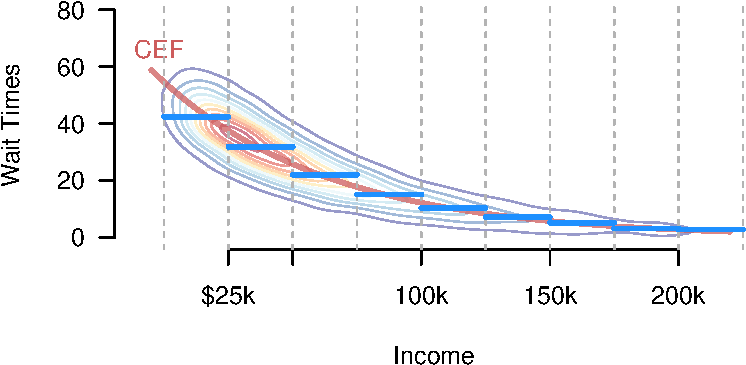
\includegraphics{linear_model_files/figure-pdf/fig-cef-binned-1.pdf}

}

\caption{\label{fig-cef-binned}Hypothetical joint distribution of income
and poll wait times (contour plot), conditional expectation function
(red), and the conditional expectation of the binned income (blue).}

\end{figure}%

Similarly, we could \textbf{assume} that the CEF follows a simple
functional form such as a line: \[ 
\mu(x) = \E[Y_{i}\mid X_{i} = x] = \beta_{0} + \beta_{1} x.
\] This assumption reduces our infinite number of unknowns (the
conditional mean at every possible income) to just two unknowns: (1) the
slope and (2) the intercept. As we will see, we can use the standard
ordinary least squares to estimate these parameters. Note that if the
true CEF is nonlinear, this assumption is incorrect, and any estimate
based on this assumption might be biased or even inconsistent.

We call the binning and linear assumptions on \(\mu(x)\)
\textbf{functional form} assumptions because they restrict the class of
functions that \(\mu(x)\) can take. While powerful, these types of
assumptions can muddy the roles of defining the quantity of interest and
estimation. If our estimator \(\widehat{\mu}(x)\) performs poorly, it
will be difficult to tell if this is because the estimator is flawed or
our functional form assumptions are incorrect.

To clarify these issues, we will pursue a different approach:
understanding what linear regression can estimate under minimal
assumptions and then investigating how well this estimand approximates
the true CEF.

\section{Population linear regression}\label{sec-linear-projection}

\subsection{Bivariate linear
regression}\label{bivariate-linear-regression}

Let's set aside the idea of the conditional expectation function and
instead focus on finding the \textbf{linear} function of a single
covariate \(X_i\) that best predicts the outcome. Recall from your
earlier mathematical training that linear functions have the form
\(a + bX_i\). The \textbf{best linear predictor} (BLP) or
\textbf{population linear regression} of \(Y_i\) on \(X_i\) is defined
as \[ 
m(x) = \beta_0 + \beta_1 x \quad\text{where, }\quad (\beta_{0}, \beta_{1}) = \argmin_{(b_{0}, b_{1}) \in \mathbb{R}^{2}}\; \E[(Y_{i} - b_{0} - b_{1}X_{i} )^{2}].
\] The expression being minimized is the expected prediction error, or
the (squared) distance between the observed outcome and the outcome as
predicted with a particular slope and intercept. The best linear
predictor is the line (that is, slope and intercept values) that results
in the lowest expected prediction error. Note that this function is a
feature of the joint distribution of the data---the DGP---and so we
cannot observe it directly. It must be estimated. The BLP is an
alternative to the CEF for summarizing the relationship between the
outcome and the covariate, though as we discuss later they will
sometimes be equal. We call \((\beta_{0}, \beta_{1})\) the
\textbf{population linear regression coefficients}. Note that \(m(x)\)
could differ greatly from the CEF \(\mu(x)\) if the latter is nonlinear.

We can solve for the best linear predictor using standard calculus
(taking the derivative with respect to each coefficient, setting those
equations equal to 0, and solving the system of equations). The
first-order conditions, in this case, are \[ 
\begin{aligned}
  \frac{\partial \E[(Y_{i} - b_{0} - b_{1}X_{i} )^{2}]}{\partial b_{0}} = \E[-2(Y_{i} - \beta_{0} - \beta_{1}X_{i})] = 0 \\
  \frac{\partial \E[(Y_{i} - b_{0} - b_{1}X_{i} )^{2}]}{\partial b_{1}} = \E[-2(Y_{i} - \beta_{0} - \beta_{1}X_{i})X_{i}] = 0
\end{aligned}  
\] Given the linearity of expectations, it is easy to solve for
\(\beta_0\) in terms of \(\beta_1\), \[ 
\beta_{0} = \E[Y_{i}] - \beta_{1}\E[X_{i}].
\] We can plug this into the first-order condition for \(\beta_1\) to
get \[ 
\begin{aligned}
  0 &= \E[Y_{i}X_{i}] - (\E[Y_{i}] - \beta_{1}\E[X_{i}])\E[X_{i}] - \beta_{1}\E[X_{i}^{2}] \\
    &= \E[Y_{i}X_{i}] - \E[Y_{i}]\E[X_{i}] - \beta_{1}(\E[X_{i}^{2}] - \E[X_{i}]^{2}) \\
    &= \cov(X_{i},Y_{i}) - \beta_{1}\V[X_{i}]\\
  \beta_{1} &= \frac{\cov(X_{i},Y_{i})}{\V[X_{i}]}
\end{aligned}
\]

Thus, the slope on the population linear regression of \(Y_i\) on
\(X_i\) is equal to the ratio of the covariance of the two variables
divided by the variance of \(X_i\). It follows from this that the
covariance will determine the sign of the slope: positive covariances
will lead to positive \(\beta_1\) and negative covariances will lead to
negative \(\beta_1\). In addition, if \(Y_i\) and \(X_i\) are
independent, \(\beta_1 = 0\). The slope scales this covariance by the
variance of the covariate, so slopes will be lower for more spread-out
covariates and higher for less spread-out covariates. If we define the
correlation between these variables as \(\rho_{YX}\), then we can relate
the coefficient to this quantity as \[
\beta_1 = \rho_{YX}\sqrt{\frac{\V[Y_i]}{\V[X_i]}}.
\]

Collecting these various results together, we can write the population
linear regression as \[
m(x) = \beta_0 + \beta_1x = \E[Y_i] + \beta_1(x - \E[X_i]),
\] which shows how we adjust our best guess about \(Y_i\) from the mean
of the outcome using the covariate.

Be sure to remember that the BLP, \(m(x)\), and the CEF, \(\mu(x)\), are
distinct entities. If the CEF is nonlinear, as in
Figure~\ref{fig-cef-blp}, there will be a difference between these
functions, meaning that the BLP might produce subpar predictions. We
will derive a formal connection between the BLP and the CEF below.

\begin{figure}[th]

\centering{

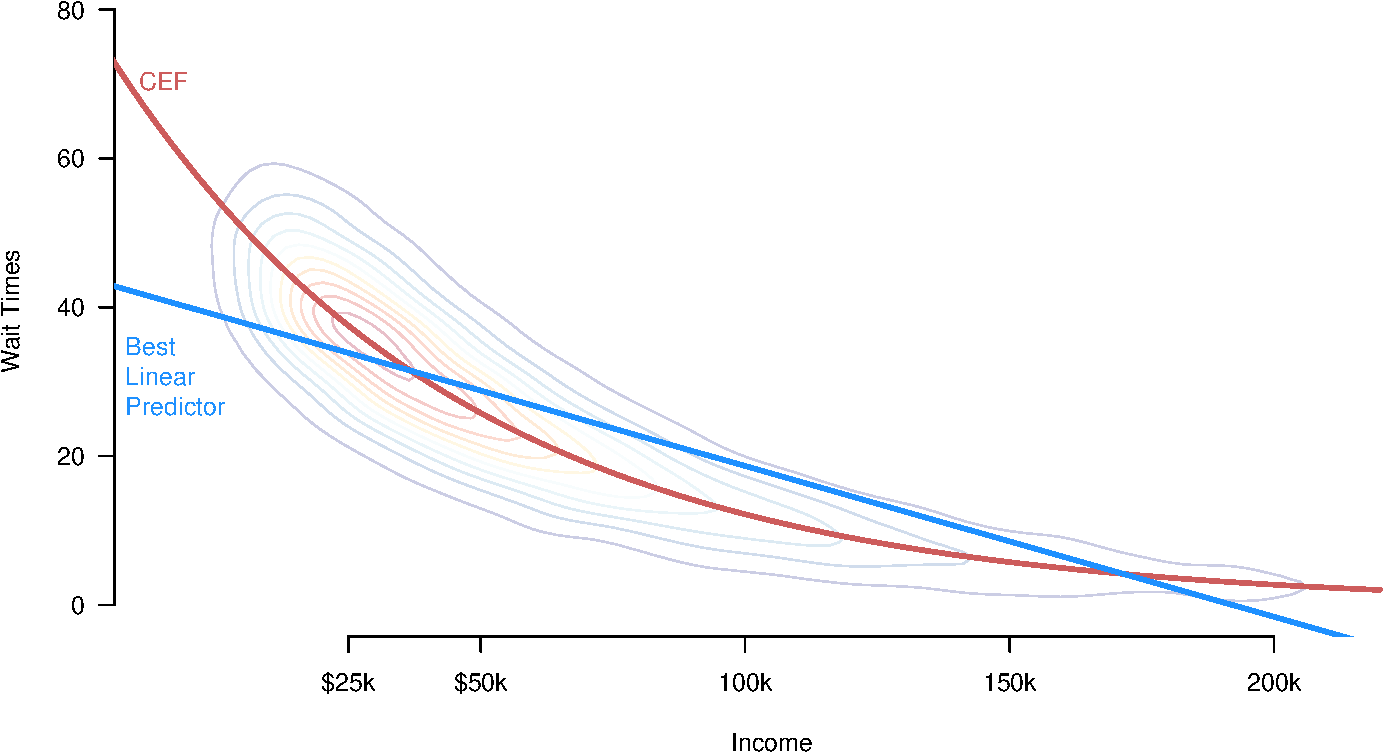
\includegraphics{linear_model_files/figure-pdf/fig-cef-blp-1.pdf}

}

\caption{\label{fig-cef-blp}Comparison of the CEF and the best linear
predictor.}

\end{figure}%

\subsection{Beyond linear
approximations}\label{beyond-linear-approximations}

The linear part of the ``best linear predictor'' is less restrictive
than it appears at first glance. We can easily modify the minimum MSE
problem to find the best quadratic, cubic, or general polynomial
function of \(X_i\) that predicts \(Y_i\). For example, the quadratic
function of \(X_i\) that best predicts \(Y_i\) would be \[ 
m(X_i, X_i^2) = \beta_0 + \beta_1X_i + \beta_2X_i^2 \quad\text{where}\quad \argmin_{(b_0,b_1,b_2) \in \mathbb{R}^3}\;\E[(Y_{i} - b_{0} - b_{1}X_{i} - b_{2}X_{i}^{2})^{2}].
\] While the equation is now a quadratic function of the covariates, it
is still a linear function of the unknown parameters
\((\beta_{0}, \beta_{1}, \beta_{2})\), so we still call this a best
linear predictor.

We could include higher-order terms of \(X_i\) in the same manner, and,
including more polynomial terms, \(X_i^p\), will allow the BLP to be a
more flexible function of \(X_i\). When we estimate the BLP, however, we
usually pay for this flexibility with overfitting and high variance in
our estimates.

\subsection{Linear prediction with multiple
covariates}\label{linear-prediction-with-multiple-covariates}

We now generalize the idea of a best linear predictor to a setting with
an arbitrary number of covariates, which more flexibly captures
real-life empirical research scenarios. In this setting, recall that the
linear function will be

\[ 
\bfx'\bfbeta = x_{1}\beta_{1} + x_{2}\beta_{2} + \cdots + x_{k}\beta_{k}.
\] We will define the \textbf{best linear predictor} (BLP) to be \[ 
m(\bfx) = \bfx'\bfbeta, \quad \text{where}\quad \bfbeta = \argmin_{\mb{b} \in \real^k}\; \E\bigl[ \bigl(Y_{i} - \mb{X}_{i}'\mb{b} \bigr)^2\bigr]
\]

This BLP solves the same fundamental optimization problem as in the
bivariate case: it chooses the set of coefficients that minimizes the
expected mean-squared error, where the expectation is over the joint
distribution of the data.

\begin{tcolorbox}[enhanced jigsaw, toptitle=1mm, bottomrule=.15mm, leftrule=.75mm, rightrule=.15mm, breakable, colframe=quarto-callout-note-color-frame, title=\textcolor{quarto-callout-note-color}{\faInfo}\hspace{0.5em}{Best linear projection assumptions}, colbacktitle=quarto-callout-note-color!10!white, titlerule=0mm, coltitle=black, left=2mm, colback=white, bottomtitle=1mm, opacitybacktitle=0.6, opacityback=0, toprule=.15mm, arc=.35mm]

Without some assumptions on the joint distribution of the data, the
following ``regularity conditions'' will ensure the existence of the
BLP:

\begin{enumerate}
\def\labelenumi{\arabic{enumi}.}
\tightlist
\item
  \(\E[Y^2] < \infty\) (outcome has finite mean/variance)
\item
  \(\E\Vert \mb{X} \Vert^2 < \infty\) (\(\mb{X}\) has finite
  means/variances/covariances)
\item
  \(\mb{Q}_{\mb{XX}} = \E[\mb{XX}']\) is positive definite (columns of
  \(\X\) are linearly independent)\\
\end{enumerate}

\end{tcolorbox}

Under these assumptions, it is possible to derive a closed-form
expression for the \textbf{population coefficients} \(\bfbeta\) using
matrix calculus. To set up the optimization problem, we find the
first-order condition by taking the derivative of the expectation of the
squared errors. First, take the derivative of the squared prediction
errors using the chain rule: \[ 
\begin{aligned}
  \frac{\partial}{\partial \mb{b}}\left(Y_{i} - \X_{i}'\mb{b}\right)^{2}
  &= 2\left(Y_{i} - \X_{i}'\mb{b}\right)\frac{\partial}{\partial \mb{b}}(Y_{i} - \X_{i}'\mb{b}) \\
  &= -2\left(Y_{i} - \X_{i}'\mb{b}\right)\X_{i} \\
  &= -2\X_{i}\left(Y_{i} - \X_{i}'\mb{b}\right) \\
  &= -2\left(\X_{i}Y_{i} - \X_{i}\X_{i}'\mb{b}\right),
\end{aligned}
\] where the third equality comes from the fact that
\((Y_{i} - \X_{i}'\bfbeta)\) is a scalar. We can plug this into the
expectation to get the first-order condition and solve for \(\bfbeta\),
\[ 
\begin{aligned}
  0 &= -2\E[\X_{i}Y_{i} - \X_{i}\X_{i}'\bfbeta ] \\
  \E[\X_{i}\X_{i}'] \bfbeta &= \E[\X_{i}Y_{i}],
\end{aligned}
\] which implies the population coefficients are \[ 
\bfbeta = \left(\E[\X_{i}\X_{i}']\right)^{-1}\E[\X_{i}Y_{i}] = \mb{Q}_{\mb{XX}}^{-1}\mb{Q}_{\mb{X}Y}
\] This gives us an expression for the coefficients for the population
best linear predictor in terms of the joint distribution
\((Y_{i}, \X_{i})\).

A couple of facts might be useful for interpreting this expression
substantively. Recall that \(\mb{Q}_{\mb{XX}} = \E[\X_{i}\X_{i}']\) is a
\(k\times k\) matrix and \(\mb{Q}_{\X Y} = \E[\X_{i}Y_{i}]\) is a
\(k\times 1\) column vector, which implies that \(\bfbeta\) is also a
\(k \times 1\) column vector.

\begin{tcolorbox}[enhanced jigsaw, toptitle=1mm, bottomrule=.15mm, leftrule=.75mm, rightrule=.15mm, breakable, colframe=quarto-callout-note-color-frame, title=\textcolor{quarto-callout-note-color}{\faInfo}\hspace{0.5em}{Note}, colbacktitle=quarto-callout-note-color!10!white, titlerule=0mm, coltitle=black, left=2mm, colback=white, bottomtitle=1mm, opacitybacktitle=0.6, opacityback=0, toprule=.15mm, arc=.35mm]

What does the expression for the population regression coefficients
mean? It is helpful to separate the intercept or constant term so that
we have \[ 
Y_{i} = \beta_{0} + \X'\bfbeta + e_{i},
\] so \(\bfbeta\) refers to just the vector of coefficients for the
covariates. In this case, we can write the coefficients in a more
interpretable way: \[ 
\bfbeta = \V[\X]^{-1}\text{Cov}(\X, Y), \qquad \beta_0 = \mu_Y - \mb{\mu}'_{\mb{X}}\bfbeta
\]

Thus, the population coefficients take the covariance between the
outcome and the covariates and ``divide'' it by information about
variances and covariances of the covariates. The intercept recenters the
regression so that projection errors are mean zero. This means that
these coefficients generalize the bivariate formula to this multiple
covariate context.

\end{tcolorbox}

With an expression for the population linear regression coefficients, we
can write the linear projection as \[ 
m(\X_{i}) = \X_{i}'\left(\E[\X_{i}\X_{i}']\right)^{-1}\E[\X_{i}Y_{i}] = \X_{i}'\mb{Q}_{\mb{XX}}^{-1}\mb{Q}_{\mb{X}Y}
\]

\subsection{Projection error}\label{projection-error}

The \textbf{projection error} or is the difference between the actual
value of \(Y_i\) and the projection, \[ 
e_{i} = Y_{i} - m(\X_{i}) = Y_i - \X_{i}'\bfbeta,
\] where we have made no assumptions about this error yet. The
projection error is simply the prediction error of the best linear
prediction for a particular unit in the data. Rewriting this definition,
we can see that we can always write the outcome as the linear projection
plus the projection error, \[ 
Y_{i} = \X_{i}'\bfbeta + e_{i}.
\] Notice that this looks suspiciously similar to a linearity assumption
on the CEF, but we haven't made any assumptions here. Instead, we just
used the definition of the projection error to write a tautological
statement: \[ 
Y_{i} = \X_{i}'\bfbeta + e_{i} = \X_{i}'\bfbeta + Y_{i} - \X_{i}'\bfbeta = Y_{i}.
\] The critical difference between this representation and the usual
linear model assumption is what properties \(e_{i}\) possesses.

A key property of the projection errors is that when the covariate
vector includes an ``intercept'' or constant term, the projection errors
are uncorrelated with the covariates. To see this, first note that
\(\E[\X_{i}e_{i}] = 0\) since \[ 
\begin{aligned}
  \E[\X_{i}e_{i}] &= \E[\X_{{i}}(Y_{i} - \X_{i}'\bfbeta)] \\
                  &= \E[\X_{i}Y_{i}] - \E[\X_{i}\X_{i}']\bfbeta \\
                  &= \E[\X_{i}Y_{i}] - \E[\X_{i}\X_{i}']\left(\E[\X_{i}\X_{i}']\right)^{-1}\E[\X_{i}Y_{i}] \\
  &= \E[\X_{i}Y_{i}] - \E[\X_{i}Y_{i}] = 0
\end{aligned}
\] Thus, for every \(X_{ij}\) in \(\X_{i}\), we have
\(\E[X_{ij}e_{i}] = 0\). If one of the entries in \(\X_i\) is a constant
1, then this also implies that \(\E[e_{i}] = 0\). Together, these facts
imply that the projection error is uncorrelated with each \(X_{ij}\),
since \[ 
\cov(X_{ij}, e_{i}) = \E[X_{ij}e_{i}] - \E[X_{ij}]\E[e_{i}] = 0 - 0 = 0
\] Note that we still have made no assumptions about these projection
errors except for some mild regularity conditions on the joint
distribution of the outcome and covariates. Thus, in very general
settings, we can write the linear projection model
\(Y_i = \X_i'\bfbeta + e_i\) where
\(\bfbeta = \left(\E[\X_{i}\X_{i}']\right)^{-1}\E[\X_{i}Y_{i}]\) and
conclude that \(\E[\X_{i}e_{i}] = 0\) by definition, not by assumption.

The projection error is uncorrelated with the covariates, so does this
mean that the CEF is linear? Unfortunately, no. Recall that while
independence implies this lack of correlation, the reverse does not
hold. So when we look at the CEF, we have \[ 
\E[Y_{i} \mid \X_{i}] = \X_{i}'\bfbeta + \E[e_{i} \mid \X_{i}],
\] and the last term \(\E[e_{i} \mid \X_{i}]\) would only be 0 if the
errors were independent of the covariates, so
\(\E[e_{i} \mid \X_{i}] = \E[e_{i}] = 0\). But nowhere in the linear
projection model did we assume this. So while we can (almost) always
write the outcome as \(Y_i = \X_i'\bfbeta + e_i\) and have those
projection errors be uncorrelated with the covariates, it will require
additional assumptions to ensure that the true CEF is, in fact, linear
\(\E[Y_{i} \mid \X_{i}] = \X_{i}'\bfbeta\).

To step back for a moment, what have we shown here? In a nutshell, we
showed that a population linear regression exists under very general
conditions and that we can write the coefficients of that population
linear regression as a function of expectations of the joint
distribution of the data. We did not, however, assume that the CEF was
linear nor that the projection errors were normally distributed.

Why is this important? The ordinary least squares estimator, the
workhorse regression estimator of the social sciences, targets this
quantity of interest in large samples, regardless of whether the true
CEF is linear or not. Thus, even when a linear CEF assumption is
incorrect and the projection errors are not normally distributed, OLS
still targets a perfectly valid quantity of interest: the coefficients
from this population linear projection.

\section{Linear CEFs without
assumptions}\label{linear-cefs-without-assumptions}

What is the relationship between the best linear predictor (which we
just saw generally exists) and the CEF? To draw the connection, remember
that the conditional expectation is importantly the function of \(\X_i\)
that best predicts \(Y_{i}\). The population regression was the best
\textbf{linear} predictor, but the CEF is the best predictor among all
nicely behaved functions of \(\X_{i}\), linear or nonlinear. In
particular, if we label \(L_2\) to be the set of all functions of the
covariates \(g()\) that have finite squared expectation,
\(\E[g(\X_{i})^{2}] < \infty\), then we can show that the CEF has the
lowest squared prediction error in this class of functions: \[ 
\mu(\X) = \E[Y_{i} \mid \X_{i}] = \argmin_{g(\X_i) \in L_2}\; \E\left[(Y_{i} - g(\X_{i}))^{2}\right],
\]

So we have established that the CEF is the best predictor and the
population linear regression \(m(\X_{i})\) is the best linear predictor.
These two facts allow us to connect the CEF to the population
regression.

\begin{theorem}[]\protect\hypertarget{thm-cef-blp}{}\label{thm-cef-blp}

If \(\mu(\X_{i})\) is a linear function of \(\X_i\), then
\(\mu(\X_{i}) = m(\X_{i}) = \X_i'\bfbeta\).

\end{theorem}

This theorem says that if the true CEF is linear, it must equal the
population linear regression. The proof of this is straightforward: the
CEF is the best predictor, so if it is linear, it must also be the best
linear predictor.

In general, we are in the business of learning about the CEF, so we are
unlikely to know if it genuinely is linear or not. In some situations,
however, we can show that the CEF is linear without any additional
assumptions. These are situations where the covariates take on a finite
number of possible values. Going back to the example from the chapter
introduction, suppose we are interested in the CEF of wait times at
voting precincts for Black (\(X_i = 1\)) vs.~non-Black (\(X_i = 0\))
voters. In this case, there are two possible values of the CEF,
\(\mu(1) = \E[Y_{i}\mid X_{i}= 1]\), the average wait time for Black
voters, and \(\mu(0) = \E[Y_{i}\mid X_{i} = 0]\), the average wait time
for non-Black voters. Notice that we can write the CEF as \[ 
\mu(x) = x \mu(1) + (1 - x) \mu(0) = \mu(0) + x\left(\mu(1) - \mu(0)\right)= \beta_0 + x\beta_1,
\] which is clearly a linear function of \(x\). Based on this
derivation, we obtain coefficients of this linear CEF that have clear
substantive interpretations:

\begin{itemize}
\tightlist
\item
  \(\beta_0 = \mu(0)\): the expected wait time for a Black voter.
\item
  \(\beta_1 = \mu(1) - \mu(0)\): the difference in average wait times
  between Black and non-Black voters. How \(X_{i}\) is defined here is
  important since the intercept will always be the average outcome when
  \(X_i = 0\), and the slope will always be the difference in means
  between the \(X_i = 1\) group and the \(X_i = 0\) group.
\end{itemize}

What about a categorical covariate with more than two levels? For
example, we may be interested in wait times by party identification,
where \(X_i = 1\) indicates Democratic voters, \(X_i = 2\) indicates
Republican voters, and \(X_i = 3\) indicates Independent voters. We
could write the CEF of wait times as a linear function of this variable,
but that would assume that the difference between Democrats and
Republicans is exactly the same as for Independents and Republicans --
which is probably false. With more than two levels, we can represent a
categorical variable as a vector of binary variables,
\(\X_i = (X_{i1}, X_{i2})\), where \[ 
\begin{aligned}
  X_{{i1}} &= \begin{cases}
                1&\text{if Republican} \\
                   0 & \text{if not Republican}
              \end{cases} \\
X_{{i2}} &= \begin{cases}
                1&\text{if independent} \\
                   0 & \text{if not independent}
              \end{cases} \\
\end{aligned}
\] These two indicator variables encode the same information as the
original single three-level variable, \(X_{i}\), so if we know the
values of \(X_{i1}\) and \(X_{i2}\), then we know exactly to which party
\(i\) belongs. Thus, the CEFs for \(X_i\) and the pair of indicator
variables, \(\X_i\), are precisely the same, but the latter allows for a
lovely linear representation, \[
\E[Y_i \mid X_{i1}, X_{i2}] = \beta_0 + \beta_1 X_{i1} + \beta_2 X_{i2},
\] where

\begin{itemize}
\tightlist
\item
  \(\beta_0 = \E[Y_{i} \mid X_{i1} = 0, X_{i2} = 0]\) is the average
  wait time for the group who does not get an indicator variable
  (Democrats in this case). This group is sometimes called the baseline
  group or the omitted group.
\item
  \(\beta_1 = \E[Y_{i} \mid X_{i1} = 1, X_{i2} = 0] - \E[Y_{i} \mid X_{i1} = 0, X_{i2} = 0]\)
  is the difference in means between Republican voters and Democratic
  voters, or the difference between the first indicator group and the
  baseline group.
\item
  \(\beta_2 = \E[Y_{i} \mid X_{i1} = 0, X_{i2} = 1] - \E[Y_{i} \mid X_{i1} = 0, X_{i2} = 0]\)
  is the difference in means between independent voters and Democratic
  voters, or the difference between the second indicator group and the
  baseline group.
\end{itemize}

This approach easily generalizes to categorical variables with an
arbitrary number of levels.

What have we shown? The CEF is linear without additional assumptions
when there is a categorical covariate. We can show that this continues
to hold even when we have multiple categorical variables. We now have
two binary covariates: \(X_{i1}=1\) indicating a Black voter, and
\(X_{i2} = 1\) indicating a retired voter versus a working-age voter.
These two binary variables give us four possible values of the CEF: \[ 
\mu(x_1, x_2) = \begin{cases} 
 \mu_{00} & \text{if } x_1 = 0 \text{ and } x_2 = 0 \text{ (non-Black, working age)} \\
 \mu_{10} & \text{if } x_1 = 1 \text{ and } x_2 = 0 \text{ (Black, working age)} \\
 \mu_{01} & \text{if } x_1 = 0 \text{ and } x_2 = 1 \text{ (non-Black, retired)} \\
 \mu_{11} & \text{if } x_1 = 1 \text{ and } x_2 = 1 \text{ (Black, retired)}
 \end{cases}
\] We can write this as \[ 
\mu(x_{1}, x_{2}) = (1 - x_{1})(1 - x_{2})\mu_{00} + x_{1}(1 -x_{2})\mu_{10} + (1-x_{1})x_{2}\mu_{01} + x_{1}x_{2}\mu_{11},
\] which we can rewrite as \[ 
\mu(x_1, x_2) = \beta_0 + x_1\beta_1 + x_2\beta_2 + x_1x_2\beta_3,
\] where the substantive interpretations are

\begin{itemize}
\tightlist
\item
  \(\beta_0 = \mu_{00}\): average wait times for working-age non-Black
  voters.
\item
  \(\beta_1 = \mu_{10} - \mu_{00}\): difference in means for working-age
  Black vs.~working-age non-Black voters.
\item
  \(\beta_2 = \mu_{01} - \mu_{00}\): difference in means for retired
  non-Black vs.~working-age non-Black voters.
\item
  \(\beta_3 = (\mu_{11} - \mu_{01}) - (\mu_{10} - \mu_{00})\):
  difference in retired racial difference vs working-age racial
  difference.
\end{itemize}

Thus, we can write the CEF with two binary covariates as linear when the
linear specification includes a multiplicative interaction between them
(\(x_1x_2\)). This result holds for all pairs of binary covariates, and
we can generalize the interpretation of the coefficients in the CEF as

\begin{itemize}
\tightlist
\item
  \(\beta_0 = \mu_{00}\): average outcome when both variables are 0.
\item
  \(\beta_1 = \mu_{10} - \mu_{00}\): difference in average outcomes for
  the first covariate when the second covariate is 0.
\item
  \(\beta_2 = \mu_{01} - \mu_{00}\): difference in average outcomes for
  the second covariate when the first covariate is 0.
\item
  \(\beta_3 = (\mu_{11} - \mu_{01}) - (\mu_{10} - \mu_{00})\): change in
  the ``effect'' of the first (second) covariate when the second (first)
  covariate goes from 0 to 1.
\end{itemize}

This result also generalizes to an arbitrary number of binary
covariates. If we have \(p\) binary covariates, then the CEF will be
linear with all two-way interactions, \(x_1x_2\), all three-way
interactions, \(x_1x_2x_3\), up to the \(p\)-way interaction
\(x_1\times\cdots\times x_p\). Furthermore, we can generalize to
arbitrary numbers of categorical variables by expanding each into a
series of binary variables and then including all interactions between
the resulting binary variables.

We have established that when we have a set of categorical covariates,
the true CEF will be linear, and we have seen the various ways to
represent that CEF. Note that when we use, for example, ordinary least
squares, we are free to choose how to include our variables. We could
run a regression of \(Y_i\) on \(X_{i1}\) and \(X_{i2}\) without an
interaction term, but this model will only be correct if \(\beta_3\) is
equal to 0, and so the interaction term is irrelevant. We call a model
\textbf{saturated} if there are as many coefficients as the CEF's unique
values. A saturated model can, by its nature, always be written as a
linear function without assumptions. The above examples show how to
construct saturated models in various situations.

\section{Interpretation of the regression
coefficients}\label{interpretation-of-the-regression-coefficients}

We have seen how to interpret population regression coefficients when
the CEF is linear without assumptions. How do we interpret the
population coefficients \(\bfbeta\) in other settings?

Consider the simplest case, one in which every entry in \(\X_{i}\)
represents a different covariate and no covariate is any function of
another (we will see why this caveat is necessary below). In this simple
case, the \(k\)th coefficient, \(\beta_{k}\), represents the change in
the predicted outcome for a one-unit change in the \(k\)th covariate
\(X_{ik}\), holding all other covariates fixed. We can see this from \[ 
\begin{aligned}
  m(x_{1} + 1, x_{2}) & = \beta_{0} + \beta_{1}(x_{1} + 1) + \beta_{2}x_{2} \\
  m(x_{1}, x_{2}) &= \beta_{0} + \beta_{1}x_{1} + \beta_{2}x_{2},
\end{aligned} 
\] so that the change in the predicted outcome for increasing \(X_{i1}\)
by one unit is \[
 m(x_{1} + 1, x_{2}) - m(x_{1}, x_{2}) = \beta_1
\] Notice that nothing changes in this interpretation when adding more
covariates to the vector, \[
 m(x_{1} + 1, \bfx_{2}) - m(x_{1}, \bfx_{2}) = \beta_1,
\] The coefficient on a particular variable is the change in the
predicted outcome corresponding to a one-unit change in the covariate
holding all other covariates constant. Each coefficient summarizes the
``all else equal'' difference in the predicted outcome for each
covariate.

\subsection{Polynomial functions of the
covariates}\label{polynomial-functions-of-the-covariates}

The interpretation of the population regression coefficients becomes
more complicated when including nonlinear functions of the covariates.
In that case, multiple coefficients control how a change in a covariate
will change the predicted value of \(Y_i\). For example, suppose we have
a quadratic function of \(X_{i1}\), \[ 
m(x_1, x_1^2, x_{2}) = \beta_{0} + \beta_{1}x_{1} + \beta_{2}x_{1}^{2} + \beta_{3}x_{2},
\] and try to look at a one-unit change in \(x_1\), \[ 
\begin{aligned}
  m(x_{1} + 1, (x_{1} + 1)^{2}, x_{2}) & = \beta_{0} + \beta_{1}(x_{1} + 1) + \beta_{2}(x_{1} + 1)^{2}+ \beta_{3}x_{2} \\
  m(x_{1}, x_{1}^{2}, x_{2}) &= \beta_{0} + \beta_{1}x_{1} + \beta_{2}x_{1}^{2} + \beta_{3}x_{2},
\end{aligned} 
\] resulting in \(\beta_1 + \beta_2(2x_{1} + 1)\). This formula might be
an interesting quantity, but we more commonly use the derivative of
\(m(\bfx)\) with respect to \(x_1\) as a measure of the marginal effect
of \(X_{i1}\) on the predicted value of \(Y_i\) (holding all other
variables constant), where ``marginal'' here means the change in
prediction for a very small change in \(X_{i1}\).\footnote{Note the
  choice of language here. The marginal effect is on the predicted value
  of \(Y_i\), not on \(Y_i\) itself. So these marginal effects are
  associational, not necessarily causal quantities.} In the case of the
quadratic covariate, we have \[ 
\frac{\partial m(x_{1}, x_{1}^{2}, x_{2})}{\partial x_{1}} = \beta_{1} + 2\beta_{2}x_{1},
\] so the marginal effect on prediction varies as a function of \(x_1\).
From this, we see that the individual interpretations of the
coefficients are less interesting: \(\beta_1\) is the marginal effect
when \(X_{i1} = 0\) and \(\beta_2 / 2\) describes how a one-unit change
in \(X_{i1}\) changes the marginal effect. As is hopefully clear, it
will often be more straightforward to visualize the nonlinear predictor
function (perhaps using the orthogonalization techniques in
Section~\ref{sec-fwl}).

\subsection{Interactions}\label{interactions}

Another common nonlinear function occurs when including
\textbf{interaction terms} or covariates that are products of two other
covariates, \[ 
m(x_{1}, x_{2}, x_{1}x_{2}) = \beta_{0} + \beta_{1}x_{1} + \beta_{2}x_{2} + \beta_{3}x_{1}x_{2}.
\] In these situations, we can use the derivative of the BLP to measure
the marginal effect of one variable or the other on the predicted value
of \(Y_i\). In particular, we have \[ 
\begin{aligned}
  \frac{\partial m(x_{1}, x_{2}, x_{1}x_{2})}{\partial x_1} &= \beta_1 + \beta_3x_2, \\
  \frac{\partial m(x_{1}, x_{2}, x_{1}x_{2})}{\partial x_2} &= \beta_2 + \beta_3x_1.
\end{aligned}
\] Here, the coefficients are slightly more interpretable:

\begin{itemize}
\tightlist
\item
  \(\beta_1\): the marginal effect of \(X_{i1}\) on predicted \(Y_i\)
  when \(X_{i2} = 0\).
\item
  \(\beta_2\): the marginal effect of \(X_{i2}\) on predicted \(Y_i\)
  when \(X_{i1} = 0\).
\item
  \(\beta_3\): the change in the marginal effect of \(X_{i1}\) due to a
  one-unit change in \(X_{i2}\) \textbf{OR} the change in the marginal
  effect of \(X_{i2}\) due to a one-unit change in \(X_{i1}\).
\end{itemize}

If we add more covariates to this BLP, these interpretations change to
``holding all other covariates constant.''

Interactions are a standard part of social science research because they
allow us to assess how the relationship between the outcome and an
independent variable varies by the values of another variable. In the
context of our study of wait times at a voting precinct, if \(X_{i1}\)
is income and \(X_{i2}\) is the Black/non-Black voter indicator, then
\(\beta_3\) represents the change in the slope of the wait time-income
relationship between Black and non-Black voters.

\begin{tcolorbox}[enhanced jigsaw, toptitle=1mm, bottomrule=.15mm, leftrule=.75mm, rightrule=.15mm, breakable, colframe=quarto-callout-note-color-frame, title=\textcolor{quarto-callout-note-color}{\faInfo}\hspace{0.5em}{Centering variables to improve interpretability}, colbacktitle=quarto-callout-note-color!10!white, titlerule=0mm, coltitle=black, left=2mm, colback=white, bottomtitle=1mm, opacitybacktitle=0.6, opacityback=0, toprule=.15mm, arc=.35mm]

In many cases, the so-called marginal coefficients on the lower-order
terms (\(\beta_1\) for \(X_{i1}\) and \(\beta_2\) for \(X_{i2}\)) are
uninteresting because they represent the marginal effect of one variable
when the other is 0. If \(X_{i1}\) is age and \(X_{i2}\) is the
Black/non-Black indicator, then \(\beta_2\) is the estimated difference
in average voter wait times for voters who are zero years old, an
obviously nonsensical parameter. We can improve the interpretability of
the coefficient by recentering the age variable. Suppose we include a
mean-centered version of age, \[
\widetilde{X}_{i1} = X_{i1} - \overline{X}_1
\] in place of \(X_{i1}\). That is, we regress \(Y_i\) on
\(\widetilde{X}_{i1}\), \(X_{i2}\), and \(\widetilde{X}_{i1}X_{i2}\). In
this case, \(\beta_2\) (the coefficient on the race indicator
\(X_{i2}\)) is the marginal effect of \(X_{i2}\) when
\(\widetilde{X}_{i1} = 0\) or when \(X_{i1} = \overline{X}_1\). Thus,
this coefficient is now the estimated difference in average voter wait
times for the average-aged voter, which is far more interpretable. This
recentering has no effect on either \(\beta_1\) or \(\beta_3\), which is
rather remarkable.

\end{tcolorbox}

\section{Multiple regression from bivariate regression}\label{sec-fwl}

With a regression of an outcome on two covariates, understanding how the
coefficients of one variable relate to the other is helpful. Consider
the following best linear projection:
\begin{equation}\phantomsection\label{eq-two-var-blp}{ 
(\alpha, \beta, \gamma) = \argmin_{(a,b,c) \in \mathbb{R}^{3}} \; \E[(Y_{i} - (a + bX_{i} + cZ_{i}))^{2}]
}\end{equation} Can we understand the \(\beta\) coefficient here in
terms of a bivariate regression? As it turns out, yes. From the above
results, we know that the intercept has a simple form: \[
\alpha = \E[Y_i] - \beta\E[X_i] - \gamma\E[Z_i].
\] Let's investigate the first order condition for \(\beta\): \[ 
\begin{aligned}
  0 &= \E[Y_{i}X_{i}] - \alpha\E[X_{i}] - \beta\E[X_{i}^{2}] - \gamma\E[X_{i}Z_{i}] \\
    &= \E[Y_{i}X_{i}] - \E[Y_{i}]\E[X_{i}] + \beta\E[X_{i}]^{2} + \gamma\E[X_{i}]\E[Z_{i}] - \beta\E[X_{i}^{2}] - \gamma\E[X_{i}Z_{i}] \\
  &= \cov(Y, X) - \beta\V[X_{i}] - \gamma \cov(X_{i}, Z_{i})
\end{aligned}
\] We can see from this that if \(\cov(X_{i}, Z_{i}) = 0\), then the
coefficient on \(X_i\) will be the same as in the simple regression
case, \(\cov(Y_{i}, X_{i})/\V[X_{i}]\). When \(X_i\) and \(Z_i\) are
uncorrelated, we sometimes call them \textbf{orthogonal}.

To write a simple formula for \(\beta\) when the covariates are not
orthogonal, we \textbf{orthogonalize} \(X_i\) by obtaining the
prediction errors from a population linear regression of \(X_i\) on
\(Z_i\): \[ 
\widetilde{X}_{i} = X_{i} - (\delta_{0} + \delta_{1}Z_{i}) \quad\text{where}\quad (\delta_{0}, \delta_{1}) = \argmin_{(d_{0},d_{1}) \in \mathbb{R}^{2}} \; \E[(X_{i} - (d_{0} + d_{1}Z_{i}))^{2}]
\] Given the properties of projection errors, we know that this
orthogonalized version of \(X_{i}\) will be uncorrelated with \(Z_{i}\)
since \(\E[\widetilde{X}_{i}Z_{i}] = 0\). Remarkably, the coefficient on
\(X_i\) from the ``long'' BLP in Equation~\ref{eq-two-var-blp} is the
same as the regression of \(Y_i\) on this orthogonalized
\(\widetilde{X}_i\), \[ 
\beta = \frac{\text{cov}(Y_{i}, \widetilde{X}_{i})}{\V[\widetilde{X}_{i}]}
\]

We can expand this idea to when there are several other covariates.
Suppose now that we are interested in a regression of \(Y_i\) on
\(\X_i\) and we are interested in the coefficient on the \(k\)th
covariate. Let \(\X_{i,-k}\) be the vector of covariates omitting the
\(k\)th entry and let \(m_k(\X_{i,-k})\) represent the BLP of \(X_{ik}\)
on these other covariates. We can define
\(\widetilde{X}_{ik} = X_{ik} - m_{k}(\X_{i,-k})\) as the \(k\)th
variable orthogonalized with respect to the rest of the variables and we
can write the coefficient on \(X_{ik}\) as \[ 
\beta_k = \frac{\cov(Y_i, \widetilde{X}_{ik})}{\V[\widetilde{X}_{ik}]}.
\] Thus, the population regression coefficient in the BLP is the same as
from a bivariate regression of the outcome on the projection error for
\(X_{ik}\) projected on all other covariates. One interpretation of
coefficients in a population multiple regression is that they represent
the relationship between the outcome and the covariate after removing
the linear relationships of all other variables.

\section{Omitted variable bias}\label{omitted-variable-bias}

In many situations, we may need to choose whether to include a variable
in a regression, so it can be helpful to understand how this choice
might affect the population coefficients on the other variables in the
regression. Suppose we have a variable \(Z_i\) that we may add to our
regression, which currently has \(\X_i\) as the covariates. We can write
this new projection as \[ 
m(\X_i, Z_i) = \X_i'\bfbeta + Z_i\gamma, \qquad m(\X_{i}) = \X_i'\bs{\delta},
\] where we often refer to \(m(\X_i, Z_i)\) as the long regression and
\(m(\X_i)\) as the short regression.

From the definition of the BLP, we can write the short coefficients as
\[ 
\bs{\delta} = \left(\E[\X_{i}\X_{i}']\right)^{-1} \E[\X_{i}Y_{i}].
\] Letting \(e_i = Y_i - m(\X_{i}, Z_{i})\) be the projection errors
from the long regression, we can write this as \[ 
\begin{aligned}
  \bs{\delta} &= \left(\E[\X_{i}\X_{i}']\right)^{-1} \E[\X_{i}(\X_{i}'\bfbeta + Z_{i}\gamma + e_{i})] \\
              &= \left(\E[\X_{i}\X_{i}']\right)^{-1}(\E[\X_{i}\X_{i}']\bfbeta + \E[\X_{i}Z_{i}]\gamma + \E[\X_{i}e_{i}]) \\
              &= \bfbeta + \left(\E[\X_{i}\X_{i}']\right)^{-1}\E[\X_{i}Z_{i}]\gamma
\end{aligned}
\] Note that the vector in the second term is the vector of linear
projection coefficients of a population linear regression of \(Z_i\) on
the \(\X_i\). If we call these coefficients \(\bs{\pi}\), then the short
coefficients are \[ 
\bs{\delta} = \bfbeta + \bs{\pi}\gamma. 
\]

We can rewrite this to show that the difference between the coefficients
in these two projections is \(\bs{\delta} - \bfbeta= \bs{\pi}\gamma\) or
the product of the coefficient on the ``excluded'' \(Z_i\) and the
coefficient of the included \(\X_i\) on the excluded. Most textbooks
refer to this difference as the \textbf{omitted variable bias} of
omitting \(Z_i\) under the idea that \(\bfbeta\) is the true target of
inference. But the result is much broader than this since it tells us
how to relate the coefficients of two nested projections.

The last two results (multiple regressions from bivariate and omitted
variable bias) are sometimes presented as results for the ordinary least
squares estimator that we will show in the next chapter. We introduce
them here as features of a particular population quantity, the linear
projection or population linear regression.

\section{Drawbacks of the BLP}\label{drawbacks-of-the-blp}

The best linear predictor is, of course, a \emph{linear} approximation
to the CEF, and this approximation could be quite poor if the true CEF
is highly nonlinear. A more subtle issue with the BLP is that it is
sensitive to the marginal distribution of the covariates when the CEF is
nonlinear. Let's return to our example of wait times at voting precincts
and income. In Figure~\ref{fig-blp-limits}, we show the true CEF and the
BLP when we restrict income below \$50,000 or above \$100,000. The BLP
can vary quite dramatically here. This figure is an extreme example, but
the essential point still holds as the marginal distribution of \(X_i\)
changes.

\begin{figure}[th]

\centering{

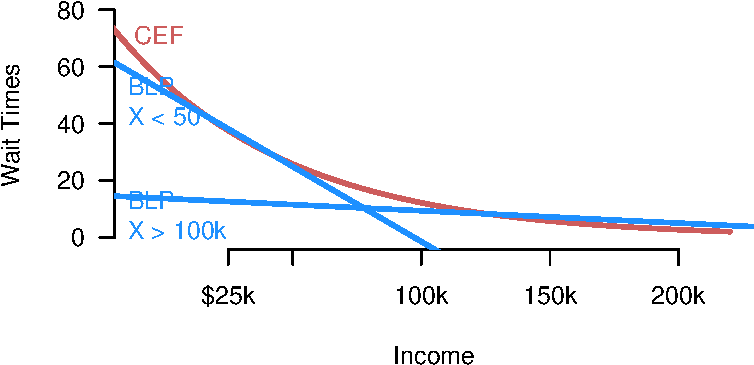
\includegraphics{linear_model_files/figure-pdf/fig-blp-limits-1.pdf}

}

\caption{\label{fig-blp-limits}Linear projections for when truncating
income distribution below \$50k and above \$100k.}

\end{figure}%

\section{Summary}\label{summary-4}

As we discussed in this chapter, with even a moderate number of
covariates, conditional expectation functions (also known as
regressions) become very difficult to estimate because of the high
dimensionality involved. To avoid this problem, we can focus on a
different quantity, the \textbf{best linear predictor} which is the
linear function of the covariates that best predicts the outcome in
mean-squared error. The BLP exists under very mild conditions and has
very interpretable parameters. Another strategy is to impose a linearity
assumption on the \textbf{conditional expectation function} to make it
more estimable, in which case, the BLP and the CEF are the same
function. With a small number of discrete covariates it is possible to
\textbf{saturate} a model so that linearity holds mechanically.
Coefficients on population linear regressions with multiple independent
variables can always be written in terms of a regression of the outcome
on one variable orthogonalized relative to the rest of the independent
variables. The \textbf{omitted variable bias} formula shows how leaving
a variable out of the best linear affects the coefficients on other
independent variables. In the next chapter, we will turn to using data
to estimate the coefficients for these population linear regressions.

\chapter{The mechanics of least squares}\label{sec-ols-mechanics}

This chapter explores the most widely used estimator for population
linear regressions: \textbf{ordinary least squares} (OLS). OLS is a
plug-in estimator for the best linear projection (or population linear
regression) described in the last chapter. Its popularity is partly due
to its ease of interpretation, computational simplicity, and statistical
efficiency. Because most people in the quantitative social sciences rely
extensively on OLS for their own research, the time you spend developing
deep familiarity with this approach will serve you well.

In this chapter, we focus on motivating the estimator and the mechanical
or algebraic properties of the OLS estimator. In the next chapter, we
will investigate its statistical assumptions. Textbooks often introduce
OLS under the assumption of a linear model for the conditional
expectation, but this is unnecessary if we view the inference target as
the best linear predictor. We discuss this point more fully in the next
chapter.

\begin{figure}[th]

\centering{

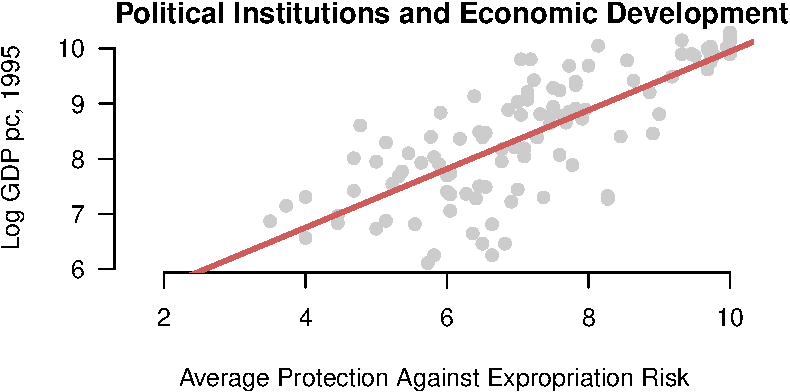
\includegraphics{least_squares_files/figure-pdf/fig-ajr-scatter-1.pdf}

}

\caption{\label{fig-ajr-scatter}Relationship between political
institutions and economic development from Acemoglu, Johnson, and
Robinson (2001).}

\end{figure}%

\section{Deriving the OLS estimator}\label{deriving-the-ols-estimator}

The last chapter on the linear model and the best linear projection
operated purely in the population, not samples. We derived the
population regression coefficients \(\bfbeta\), representing the
coefficients on the line of best fit in the population. We now take
these as our quantity of interest. We now focus on how to use a sample
from the population to make inferences about the line of best fit in the
population and the population coefficients. To do this, we will focus on
the OLS estimator for these population quantities.

\begin{tcolorbox}[enhanced jigsaw, toptitle=1mm, bottomrule=.15mm, leftrule=.75mm, rightrule=.15mm, breakable, colframe=quarto-callout-note-color-frame, title=\textcolor{quarto-callout-note-color}{\faInfo}\hspace{0.5em}{Assumption}, colbacktitle=quarto-callout-note-color!10!white, titlerule=0mm, coltitle=black, left=2mm, colback=white, bottomtitle=1mm, opacitybacktitle=0.6, opacityback=0, toprule=.15mm, arc=.35mm]

The variables
\(\{(Y_1, \X_1), \ldots, (Y_i,\X_i), \ldots, (Y_n, \X_n)\}\) are i.i.d.
draws from a common distribution \(F\).

\end{tcolorbox}

Recall the population linear coefficients (or best linear predictor
coefficients) that we derived in the last chapter, \[ 
\bfbeta = \argmin_{\mb{b} \in \real^k}\; \E\bigl[ \bigl(Y_{i} - \mb{X}_{i}'\mb{b} \bigr)^2\bigr] = \left(\E[\X_{i}\X_{i}']\right)^{-1}\E[\X_{i}Y_{i}]
\]

We will consider two different ways to derive the OLS estimator for
these coefficients, both of which are versions of the plug-in principle.
The first approach is to use the closed-form representation of the
coefficients and then to replace any expectations with sample means, \[ 
\bhat = \left(\frac{1}{n} \sum_{i=1}^n \X_i\X_i' \right)^{-1} \left(\frac{1}{n} \sum_{i=1}^n \X_{i}Y_{i} \right),
\] which exists if \(\sum_{i=1}^n \X_i\X_i'\) is \textbf{positive
definite} and thus invertible. We will return to this assumption below.

In a simple bivariate linear projection model
\(m(X_{i}) = \beta_0 + \beta_1X_{i}\), we saw that the population slope
was \(\beta_1= \text{cov}(Y_{i},X_{i})/ \V[X_{i}]\). This approach means
that the estimator for the slope should be the ratio of the sample
covariance of \(Y_i\) and \(X_i\) to the sample variance of \(X_i\), or
\[ 
\widehat{\beta}_{1} = \frac{\widehat{\sigma}_{Y,X}}{\widehat{\sigma}^{2}_{X}} = \frac{ \frac{1}{n-1}\sum_{i=1}^{n} (Y_{i} - \overline{Y})(X_{i} - \overline{X})}{\frac{1}{n-1} \sum_{i=1}^{n} (X_{i} - \Xbar)^{2}}.
\]

This plug-in approach is widely applicable and tends to have excellent
properties in large samples under iid data. But the simplicity of the
plug-in approach also hides some features of the estimator that become
more apparent when deriving the estimator more explicitly using
calculus. The second approach applies the plug-in principle not to the
closed-form expression for the coefficients but to the optimization
problem itself. We call this the \textbf{least squares} estimator
because it minimizes the empirical (or sample) squared prediction error,
\[ 
\bhat = \argmin_{\mb{b} \in \real^k}\; \frac{1}{n} \sum_{i=1}^{n}\bigl(Y_{i} - \mb{X}_{i}'\mb{b} \bigr)^2 = \argmin_{\mb{b} \in \real^k}\; SSR(\mb{b}),
\] where, \[ 
SSR(\mb{b}) = \sum_{i=1}^{n}\bigl(Y_{i} - \mb{X}_{i}'\mb{b} \bigr)^2
\] is the sum of the squared residuals. To distinguish it from other,
more complicated least squares estimators, we call this the
\textbf{ordinary least squares} estimator, or OLS.

Let's solve this minimization problem. We write down the first-order
conditions as \[ 
0=\frac{\partial SSR(\bhat)}{\partial \bfbeta} = 2 \left(\sum_{i=1}^{n} \X_{i}Y_{i}\right) - 2\left(\sum_{i=1}^{n}\X_{i}\X_{i}'\right)\bhat.
\] We can rearrange this system of equations to \[ 
\left(\sum_{i=1}^{n}\X_{i}\X_{i}'\right)\bhat = \left(\sum_{i=1}^{n} \X_{i}Y_{i}\right).
\] To obtain the solution for \(\bhat\), notice that
\(\sum_{i=1}^{n}\X_{i}\X_{i}'\) is a \((k+1) \times (k+1)\) matrix and
\(\bhat\) and \(\sum_{i=1}^{n} \X_{i}Y_{i}\) are both \(k+1\) length
column vectors. If \(\sum_{i=1}^{n}\X_{i}\X_{i}'\) is invertible, then
we can multiply both sides of this equation by that inverse to arrive at
\[ 
\bhat = \left(\sum_{i=1}^n \X_i\X_i' \right)^{-1} \left(\sum_{i=1}^n \X_{i}Y_{i} \right),
\] which is the same expression as the plug-in estimator (after
canceling the \(1/n\) terms). To confirm that we have found a minimum,
we also need to check the second-order condition, \[ 
 \frac{\partial^{2} SSR(\bhat)}{\partial \bfbeta\bfbeta'} = 2\left(\sum_{i=1}^{n}\X_{i}\X_{i}'\right) > 0.
\] What does the matrix being ``positive'' mean? In matrix algebra, this
condition means that the matrix \(\sum_{i=1}^{n}\X_{i}\X_{i}'\) is
\textbf{positive definite}, a condition that we discuss in
Section~\ref{sec-rank}.

Both the plug-in or least squares approaches yield the same estimator
for the best linear predictor/population linear regression coefficients.

\begin{theorem}[]\protect\hypertarget{thm-ols}{}\label{thm-ols}

If the \(\sum_{i=1}^{n}\X_{i}\X_{i}'\) is positive definite, then the
ordinary least squares estimator is \[
\bhat = \left(\sum_{i=1}^n \X_i\X_i' \right)^{-1} \left(\sum_{i=1}^n \X_{i}Y_{i} \right).
\]

\end{theorem}

\begin{tcolorbox}[enhanced jigsaw, toptitle=1mm, bottomrule=.15mm, leftrule=.75mm, rightrule=.15mm, breakable, colframe=quarto-callout-note-color-frame, title=\textcolor{quarto-callout-note-color}{\faInfo}\hspace{0.5em}{Formula for the OLS slopes}, colbacktitle=quarto-callout-note-color!10!white, titlerule=0mm, coltitle=black, left=2mm, colback=white, bottomtitle=1mm, opacitybacktitle=0.6, opacityback=0, toprule=.15mm, arc=.35mm]

Almost all regression will contain an intercept term, usually
represented as a constant 1 in the covariate vector. It is also possible
to obtain expressions for the OLS estimates of the intercept and
variable coefficients separately. We can rewrite the best linear
predictor decomposition as \[ 
Y_{i} = \alpha + \X_{i}'\bfbeta + \e_{i}.
\] Defined this way, we can write the OLS estimator for the ``slopes''
on \(\X_i\) as the OLS estimator with all variables demeaned: \[ 
\bhat = \left(\frac{1}{n} \sum_{i=1}^{n} (\X_{i} - \overline{\X})(\X_{i} - \overline{\X})'\right) \left(\frac{1}{n} \sum_{i=1}^{n}(\X_{i} - \overline{\X})(Y_{i} - \overline{Y})\right)
\] which is the inverse of the sample covariance matrix of \(\X_i\)
times the sample covariance of \(\X_i\) and \(Y_i\). The intercept is
\[ 
\widehat{\alpha} = \overline{Y} - \overline{\X}'\bhat.
\]

\end{tcolorbox}

When dealing with actual data and not the population, we refer to the
prediction errors \(\widehat{e}_{i} = Y_i - \X_i'\bhat\) as the
\textbf{residuals}. The predicted value itself,
\(\widehat{Y}_i = \X_{i}'\bhat\), is also called the \textbf{fitted
value}. With the population linear regression, we saw that the
projection errors, \(e_i = Y_i - \X_i'\bfbeta\), were mean zero and
uncorrelated with the covariates \(\E[\X_{i}e_{i}] = 0\). The residuals
have a similar property with respect to the covariates in the sample:
\[ 
\sum_{i=1}^n \X_i\widehat{e}_i = 0.
\] The residuals are \emph{exactly} uncorrelated with the covariates
(when the covariates include a constant/intercept term), which is a
mechanical artifact of the OLS estimator.

Figure~\ref{fig-ssr-comp} shows how OLS works in the bivariate case. It
displays three possible regression lines as well as the sum of the
squared residuals for each line. OLS aims to find the line that
minimizes the function on the right.

\begin{figure}[th]

\centering{

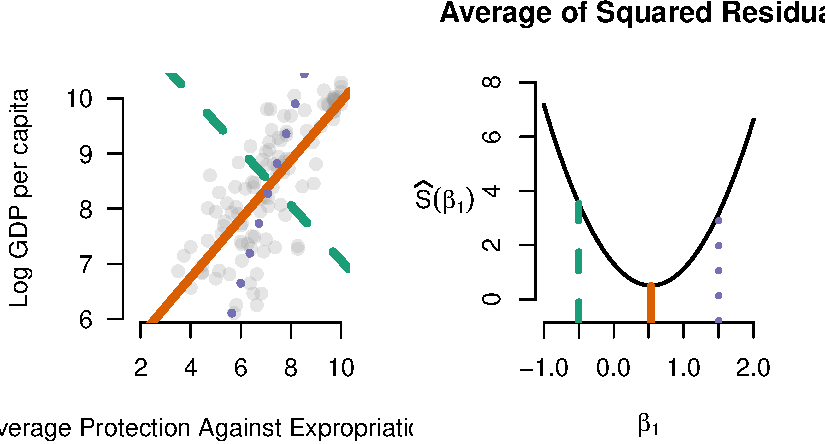
\includegraphics{least_squares_files/figure-pdf/fig-ssr-comp-1.pdf}

}

\caption{\label{fig-ssr-comp}Different possible lines and their
corresponding sum of squared residuals.}

\end{figure}%

\section{Model fit}\label{model-fit}

We have learned how to use OLS to obtain an estimate of the best linear
predictor, but an open question is whether that prediction is any good.
Does using \(\X_i\) help us predict \(Y_i\)? To investigate this, we
consider two different prediction errors: (1) those using covariates and
(2) those that do not.

We have already seen the prediction error when using the covariates; it
is just the \textbf{sum of the squared residuals}, \[ 
SSR = \sum_{i=1}^n (Y_i - \X_{i}'\bhat)^2.
\] Recall that the best predictor for \(Y_i\) without any covariates is
simply its sample mean \(\overline{Y}\). The prediction error without
covariates is what we call the \textbf{total sum of squares}, \[ 
TSS = \sum_{i=1}^n (Y_i - \overline{Y})^2.
\] Figure~\ref{fig-ssr-vs-tss} shows the difference between these two
types of prediction errors.

\begin{figure}[th]

\centering{

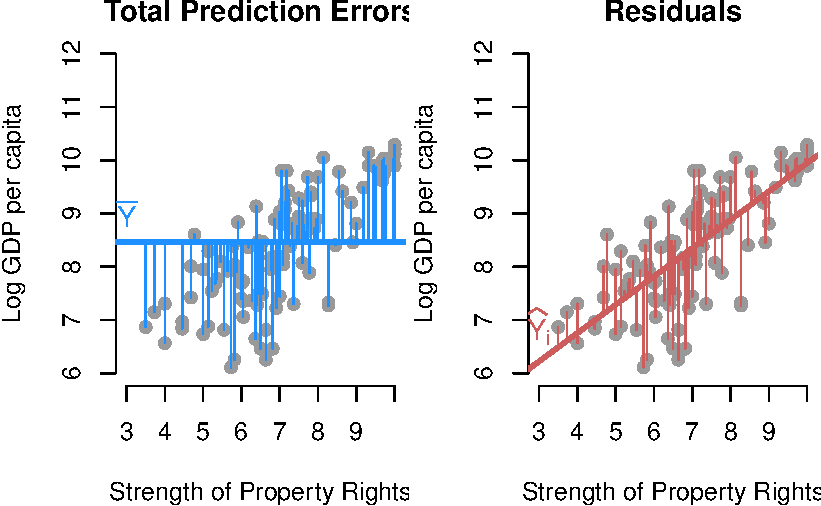
\includegraphics{least_squares_files/figure-pdf/fig-ssr-vs-tss-1.pdf}

}

\caption{\label{fig-ssr-vs-tss}Total sum of squares vs.~the sum of
squared residuals.}

\end{figure}%

We can use the \textbf{proportion reduction in prediction error} from
adding those covariates to measure how much those covariates improve the
regression's predictive ability. This value, called the
\textbf{coefficient of determination} or \(R^2\), is simply \[
R^2 = \frac{TSS - SSR}{TSS} = 1-\frac{SSR}{TSS}.
\] The numerator, \(TSS - SSR\), is the reduction in prediction error
moving from \(\overline{Y}\) to \(\X_i'\bhat\) as the predictor. The
denominator is the prediction error using \(\overline{Y}\). Thus, the
\(R^2\) value is the fraction of the total prediction error eliminated
by using \(\X_i\) to predict \(Y_i\). Another way to think about this
value is that it measures how much less noisy the residuals are relative
to the overall variation in \(Y\). One thing to note is that OLS with
covariates will \emph{always} improve in-sample fit so that
\(TSS \geq SSR\) even if \(\X_i\) is unrelated to \(Y_i\). This phantom
improvement occurs because the point of OLS is to minimize the SSR, and
it will do that even if it is just chasing noise.

Since regression always improves in-sample fit, \(R^2\) will fall
between 0 and 1. A value 0 zero would indicate exactly 0 estimated
coefficients on all covariates (except the intercept) so that \(Y_i\)
and \(\X_i\) are perfectly orthogonal in the data. (This is very
unlikely to occur because there will likely be some minimal but nonzero
relationship by random chance.) A value of 1 indicates a perfect linear
fit, which occurs when all data points are perfectly predicted by the
model with zero residuals.

\section{Matrix form of OLS}\label{matrix-form-of-ols}

We derived the OLS estimator above using simple algebra and calculus,
but a more common representation of the estimator relies on vectors and
matrices. We usually write the linear model for a generic unit,
\(Y_i = \X_i'\bfbeta + e_i\), but obviously, there are \(n\) of these
equations, \[ 
\begin{aligned}
  Y_1 &= \X_1'\bfbeta + e_1 \\
  Y_2 &= \X_2'\bfbeta + e_2 \\
  &\vdots \\
  Y_n &= \X_n'\bfbeta + e_n \\
\end{aligned}
\] We can write this system of equations more compactly using matrix
algebra. Combining the variables here into random vectors/matrices gives
us: \[
\mb{Y} = \begin{pmatrix}
Y_1 \\ Y_2 \\ \vdots \\ Y_n
  \end{pmatrix}, \quad
  \mathbb{X} = \begin{pmatrix}
\X'_1 \\
\X'_2 \\
\vdots \\
\X'_n
  \end{pmatrix} =
  \begin{pmatrix}
    1 & X_{11} & X_{12} & \cdots & X_{1k} \\
    1 & X_{21} & X_{22} & \cdots & X_{2k} \\
    \vdots & \vdots & \vdots & \vdots & \vdots \\
    1 & X_{n1} & X_{n2} & \cdots & X_{nk} \\
  \end{pmatrix},
  \quad
  \mb{e} = \begin{pmatrix}
e_1 \\ e_2 \\ \vdots \\ e_n
  \end{pmatrix}
\] We can write the above system of equations as \[
\mb{Y} = \mathbb{X}\bfbeta + \mb{e},
\] Note that \(\mathbb{X}\) is an \(n \times (k+1)\) matrix and
\(\bfbeta\) is a \(k+1\) length column vector.

Representing sums in matrix form is the critical link between the
definition of OLS and matrix notation. In particular, we have \[
\begin{aligned}
  \sum_{i=1}^n \X_i\X_i' &= \Xmat'\Xmat \\
  \sum_{i=1}^n \X_iY_i &= \Xmat'\mb{Y},
\end{aligned}
\] which means we can write the OLS estimator in the more recognizable
form as \[ 
\bhat = \left( \mathbb{X}'\mathbb{X} \right)^{-1} \mathbb{X}'\mb{Y}.
\]

We can of course also define the vector of residuals, \[ 
 \widehat{\mb{e}} = \mb{Y} - \mathbb{X}\bhat = \left[
\begin{array}{c}
    Y_1 \\
    Y_2 \\
    \vdots \\
    Y_n
    \end{array}
\right] - 
\left[
\begin{array}{c}
   1\widehat{\beta}_0 + X_{11}\widehat{\beta}_1 + X_{12}\widehat{\beta}_2 + \dots + X_{1k}\widehat{\beta}_k \\
   1\widehat{\beta}_0 + X_{21}\widehat{\beta}_1 + X_{22}\widehat{\beta}_2 + \dots + X_{2k}\widehat{\beta}_k \\
   \vdots \\
   1\widehat{\beta}_0 + X_{n1}\widehat{\beta}_1 + X_{n2}\widehat{\beta}_2 + \dots + X_{nk}\widehat{\beta}_k
\end{array}
\right],
\] and so the sum of the squared residuals in this case becomes \[ 
SSR(\bfbeta) = \Vert\mb{Y} - \mathbb{X}\bfbeta\Vert^{2} = (\mb{Y} - \mathbb{X}\bfbeta)'(\mb{Y} - \mathbb{X}\bfbeta),
\] where the double vertical lines are the Euclidean norm of the
argument, \(\Vert \mb{z} \Vert = \sqrt{\sum_{i=1}^n z_i^{2}}\). The OLS
minimization problem, then, is \[ 
\bhat = \argmin_{\mb{b} \in \mathbb{R}^{(k+1)}}\; \Vert\mb{Y} - \mathbb{X}\mb{b}\Vert^{2}
\] Finally, we can write the lack of correlation of the covariates and
the residuals as \[ 
\mathbb{X}'\widehat{\mb{e}} = \sum_{i=1}^{n} \X_{i}\widehat{e}_{i} = 0,
\] which also implies these vectors are \textbf{orthogonal}.

\section{Rank, linear independence, and
multicollinearity}\label{sec-rank}

We noted that the OLS estimator exists when \(\sum_{i=1}^n \X_i\X_i'\)
is positive definite or that there is ``no multicollinearity.'' This
assumption is equivalent to saying that the matrix \(\mathbb{X}\) is
full column rank, meaning that \(\text{rank}(\mathbb{X}) = (k+1)\),
where \(k+1\) is the number of columns of \(\mathbb{X}\). Recall from
matrix algebra that the column rank is the number of linearly
independent columns in the matrix, and \textbf{linear independence}
means that \(\mathbb{X}\mb{b} = 0\) if and only if \(\mb{b}\) is a
column vector of 0s. In other words, we have \[ 
b_{1}\mathbb{X}_{1} + b_{2}\mathbb{X}_{2} + \cdots + b_{k+1}\mathbb{X}_{k+1} = 0 \quad\iff\quad b_{1} = b_{2} = \cdots = b_{k+1} = 0, 
\] where \(\mathbb{X}_j\) is the \(j\)th column of \(\mathbb{X}\). Thus,
full column rank says that all the columns are linearly independent or
that there is no ``multicollinearity.''

Could this be violated? Suppose we accidentally included a linear
function of one variable so that \(\mathbb{X}_2 = 2\mathbb{X}_1\). We
then have \[ 
\begin{aligned}
  \mathbb{X}\mb{b} &= b_{1}\mathbb{X}_{1} + b_{2}2\mathbb{X}_1+ b_{3}\mathbb{X}_{3}+ \cdots + b_{k+1}\mathbb{X}_{k+1} \\
  &= (b_{1} + 2b_{2})\mathbb{X}_{1} + b_{3}\mathbb{X}_{3} + \cdots + b_{k+1}\mathbb{X}_{k+1}
\end{aligned}
\] In this case, this expression equals 0 when
\(b_3 = b_4 = \cdots = b_{k+1} = 0\) and \(b_1 = -2b_2\). Thus, the
collection of columns is linearly dependent, so we know that the rank of
\(\mathbb{X}\) must be less than full column rank (that is, less than
\(k+1\)). Hopefully it is also clear that if we removed the problematic
column \(\mathbb{X}_2\), the resulting matrix would have \(k\) linearly
independent columns, implying that \(\mathbb{X}\) is rank \(k\).

Why does this rank condition matter for the OLS estimator? In short,
linear independence of the columns of \(\Xmat\) ensures that the inverse
\((\Xmat'\Xmat)^{-1}\) exists and so does \(\bhat\). This is because
\(\Xmat\) is of full column rank if and only if \(\Xmat'\Xmat\) is
non-singular and a matrix is invertible if and only if it is
non-singular. This full rank condition further implies that
\(\Xmat'\Xmat = \sum_{i=1}^{n}\X_{i}\X_{i}'\) is positive definite,
implying that the estimator is truly finding the minimal sum of squared
residuals.

What are common situations that lead to violations of no
multicollinearity? We have seen one above, with one variable being a
linear function of another. But this problem can come out in more subtle
ways. Suppose we have a set of dummy variables corresponding to a single
categorical variable, like the region of the world. This might mean we
have \(X_{i1} = 1\) for units in Asia (0 otherwise), \(X_{i2} = 1\) for
units in Europe (0 otherwise), \(X_{i3} = 1\) for units in Africa (0
otherwise), and \(X_{i4} = 1\) for units in the Americas (0 otherwise),
and \(X_{i5} = 1\) for countries in Oceania (0 otherwise). Each unit has
to be in exactly one of these five regions, so there is a linear
dependence between these variables, \[ 
X_{i5} = 1 - X_{i1} - X_{i2} - X_{i3} - X_{i4}.
\] That is, if a unit is not in Asia, Europe, Africa, or the Americas,
we know it is in Oceania. We would get a linear dependence by including
all of these variables in our regression with an intercept. (Note the 1
in the relationship between \(X_{i5}\) and the other variables, the
reason why there will be linear dependence when including a constant.)
Thus, we usually omit one dummy variable from each categorical variable.
In that case, the coefficients on the remaining dummies are differences
in means between that category and the omitted one (perhaps conditional
on other variables included, if included). So if we omitted \(X_{i5}\)
(Oceania), then the coefficient on \(X_{i1}\) would be the difference in
mean outcomes between units in Asia and Oceania.

Collinearity can also occur when including both an intercept term and a
variable that does not vary. This issue can often happen if we
mistakenly subset our data, for example in this case if we subsetted the
data to only the Asian units but still included the Asian dummy variable
in the regression.

Finally, note that most statistical software packages will ``solve'' the
multicollinearity by arbitrarily removing as many linearly dependent
covariates as is necessary to achieve full rank. R will show the
estimated coefficients as \texttt{NA} in those cases.

\section{OLS coefficients for binary and categorical
regressors}\label{ols-coefficients-for-binary-and-categorical-regressors}

Suppose that the covariates include just the intercept and a single
binary variable, \(\X_i = (1\; X_{i})'\), where \(X_i \in \{0,1\}\). In
other words, the right-hand side contains only one covariate, an
indicator variable. In this case, the OLS coefficient on \(X_i\),
\(\widehat{\beta_{1}}\), is exactly equal to the difference in sample
means of \(Y_i\) in the \(X_i = 1\) group and the \(X_i = 0\) group: \[ 
\widehat{\beta}_{1} = \frac{\sum_{i=1}^{n} X_{i}Y_{i}}{\sum_{i=1}^{n} X_{i}} - \frac{\sum_{i=1}^{n} (1 - X_{i})Y_{i}}{\sum_{i=1}^{n} 1- X_{i}} = \overline{Y}_{X =1} - \overline{Y}_{X=0}
\] This very useful result is not an approximation: it holds exactly for
any sample size.

We can generalize this idea to discrete variables more broadly. Suppose
we have our region variables from the last section and include in our
covariates a constant and the dummies for Asia, Europe, Africa, and the
Americas (with Oceania again being the omitted variable/category). Then
the coefficient on the West dummy will be \[ 
\widehat{\beta}_{\text{Asia}} = \overline{Y}_{\text{Asia}} - \overline{Y}_{\text{Oceania}},
\] which is exactly the difference in sample means of \(Y_i\) between
Asian units and units in Oceania.

Note that these interpretations only hold when the regression consists
solely of the binary variable or the set of categorical dummy variables.
These exact relationships fail when other covariates are added to the
model.

\section{Projection and geometry of least
squares}\label{projection-and-geometry-of-least-squares}

OLS has a very nice geometric interpretation that adds a lot of
intuition for various aspects of the method. In this geometric approach,
we view \(\mb{Y}\) as an \(n\)-dimensional vector in \(\mathbb{R}^n\).
As we saw above, OLS in matrix form is about finding a linear
combination of the covariate matrix \(\Xmat\) closest to this vector in
terms of the Euclidean distance, which is just the sum of squares.

Let
\(\mathcal{C}(\Xmat) = \{\Xmat\mb{b} : \mb{b} \in \mathbb{R}^(k+1)\}\)
be the \textbf{column space} of the matrix \(\Xmat\). This set is all
linear combinations of the columns of \(\Xmat\) or the set of all
possible linear predictions we could obtain from \(\Xmat\). Note that
the OLS fitted values, \(\Xmat\bhat\), are in this column space. If, as
we assume, \(\Xmat\) has full column rank of \(k+1\), then the column
space \(\mathcal{C}(\Xmat)\) will be a \(k+1\)-dimensional surface
inside of the larger \(n\)-dimensional space. If \(\Xmat\) has two
columns, the column space will be a plane.

Another interpretation of the OLS estimator is that it finds the linear
predictor as the closest point in the column space of \(\Xmat\) to the
outcome vector \(\mb{Y}\). This is called the \textbf{projection} of
\(\mb{Y}\) onto \(\mathcal{C}(\Xmat)\). Figure~\ref{fig-projection}
shows this projection for a case with \(n=3\) and 2 columns in
\(\Xmat\). The shaded blue region represents the plane of the column
space of \(\Xmat\), and \(\Xmat\bhat\) is the closest point to
\(\mb{Y}\) in that space. This illustrates the whole idea of the OLS
estimator: find the linear combination of the columns of \(\Xmat\) (a
point in the column space) that minimizes the Euclidean distance between
that point and the outcome vector (the sum of squared residuals).

\begin{figure}[th]

\centering{

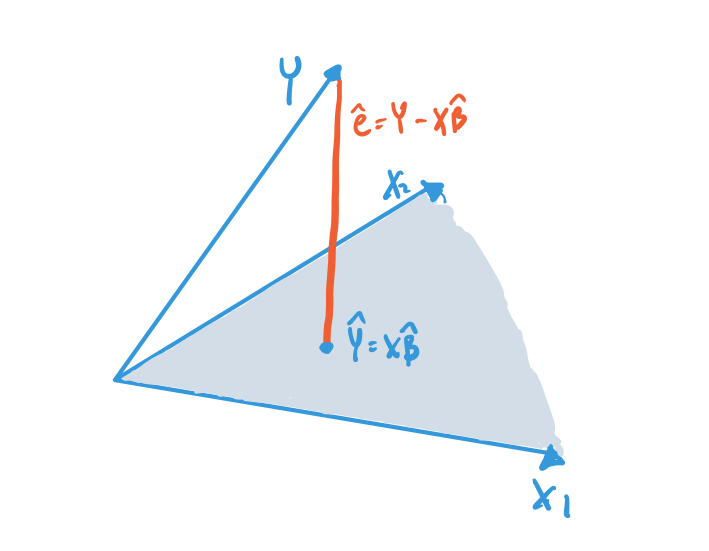
\includegraphics{assets/img/projection-drawing.png}

}

\caption{\label{fig-projection}Projection of Y on the column space of
the covariates.}

\end{figure}%

This figure shows that the residual vector, which is the difference
between the \(\mb{Y}\) vector and the projection \(\Xmat\bhat\), is
perpendicular or orthogonal to the column space of \(\Xmat\). This
orthogonality is a consequence of the residuals being orthogonal to all
the columns of \(\Xmat\), \[ 
\Xmat'\mb{e} = 0,
\] as we established above. Being orthogonal to all the columns means it
will also be orthogonal to all linear combinations of the columns.

\section{Projection and annihilator
matrices}\label{projection-and-annihilator-matrices}

With the idea of projection to the column space of \(\Xmat\)
established, we can define a way to project any vector into that space.
The \(n\times n\) \textbf{projection matrix,} \[
\mb{P}_{\Xmat} = \Xmat (\Xmat'\Xmat)^{-1} \Xmat',
\] projects a vector into \(\mathcal{C}(\Xmat)\). In particular, we can
see that this gives us the fitted values for \(\mb{Y}\): \[ 
\mb{P}_{\Xmat}\mb{Y} = \Xmat (\Xmat'\Xmat)^{-1} \Xmat'\mb{Y} = \Xmat\bhat.
\] Because we sometimes write the linear predictor as
\(\widehat{\mb{Y}} = \Xmat\bhat\), the projection matrix is also called
the \textbf{hat matrix}. With either name, multiplying a vector by
\(\mb{P}_{\Xmat}\) gives the best linear predictor of that vector as a
function of \(\Xmat\). Intuitively, any vector that is already a linear
combination of the columns of \(\Xmat\) (so is in
\(\mathcal{C}(\Xmat)\)) should be unaffected by this projection: the
closest point in \(\mathcal{C}(\Xmat)\) to a point already in
\(\mathcal{C}(\Xmat)\) is itself. We can also see this algebraically for
any linear combination \(\Xmat\mb{c}\), \[
\mb{P}_{\Xmat}\Xmat\mb{c} = \Xmat (\Xmat'\Xmat)^{-1} \Xmat'\Xmat\mb{c} = \Xmat\mb{c},
\] because \((\Xmat'\Xmat)^{-1} \Xmat'\Xmat\) simplifies to the identity
matrix. In particular, the projection of \(\Xmat\) onto itself is just
itself: \(\mb{P}_{\Xmat}\Xmat = \Xmat\).

The second matrix related to projection is the \textbf{annihilator
matrix}, \[ 
\mb{M}_{\Xmat} = \mb{I}_{n} - \mb{P}_{\Xmat},
\] which projects any vector into the orthogonal complement to the
column space of \(\Xmat\), \[
\mathcal{C}^{\perp}(\Xmat) = \{\mb{c} \in \mathbb{R}^n\;:\; \Xmat\mb{c} = 0 \}.
\] This matrix is called the annihilator matrix because applying it to
any linear combination of \(\Xmat\), gives us 0: \[ 
\mb{M}_{\Xmat}\Xmat\mb{c} = \Xmat\mb{c} - \mb{P}_{\Xmat}\Xmat\mb{c} = \Xmat\mb{c} - \Xmat\mb{c} = 0.
\] Note that \(\mb{M}_{\Xmat}\Xmat = 0\). Why should we care about this
matrix? Perhaps a more evocative name might be the \textbf{residual
maker} since it makes residuals when applied to \(\mb{Y}\), \[ 
\mb{M}_{\Xmat}\mb{Y} = (\mb{I}_{n} - \mb{P}_{\Xmat})\mb{Y} = \mb{Y} - \mb{P}_{\Xmat}\mb{Y} = \mb{Y} - \Xmat\bhat = \widehat{\mb{e}}.
\]

The projection matrix has several useful properties:

\begin{itemize}
\item
  \(\mb{P}_{\Xmat}\) and \(\mb{M}_{\Xmat}\) are \textbf{idempotent},
  which means that when applied to itself, it simply returns itself:
  \(\mb{P}_{\Xmat}\mb{P}_{\Xmat} = \mb{P}_{\Xmat}\) and
  \(\mb{M}_{\Xmat}\mb{M}_{\Xmat} = \mb{M}_{\Xmat}\).
\item
  \(\mb{P}_{\Xmat}\) and \(\mb{M}_{\Xmat}\) are symmetric \(n \times n\)
  matrices so that \(\mb{P}_{\Xmat}' = \mb{P}_{\Xmat}\) and
  \(\mb{M}_{\Xmat}' = \mb{M}_{\Xmat}\).
\item
  The rank of \(\mb{P}_{\Xmat}\) is \(k+1\) (the number of columns of
  \(\Xmat\)) and the rank of \(\mb{M}_{\Xmat}\) is \(n - k - 1\).
\end{itemize}

We can use the projection and annihilator matrices to arrive at an
orthogonal decomposition of the outcome vector: \[ 
\mb{Y} = \Xmat\bhat + \widehat{\mb{e}} = \mb{P}_{\Xmat}\mb{Y} + \mb{M}_{\Xmat}\mb{Y}.
\]

\section{Residual regression}\label{residual-regression}

There are many situations where we can partition the covariates into two
groups, and we might wonder if it is possible to express or calculate
the OLS coefficients for just one set of covariates. In particular, let
the columns of \(\Xmat\) be partitioned into \([\Xmat_{1} \Xmat_{2}]\),
so that the linear prediction we are estimating is \[ 
\mb{Y} = \Xmat_{1}\bfbeta_{1} + \Xmat_{2}\bfbeta_{2} + \mb{e}, 
\] with estimated coefficients and residuals \[ 
\mb{Y} = \Xmat_{1}\bhat_{1} + \Xmat_{2}\bhat_{2} + \widehat{\mb{e}}.
\]

We now document another way to obtain the estimator \(\bhat_1\) from
this regression using a technique called \textbf{residual regression},
\textbf{partitioned regression}, or the \textbf{Frisch-Waugh-Lovell
theorem}.

\begin{tcolorbox}[enhanced jigsaw, toptitle=1mm, bottomrule=.15mm, leftrule=.75mm, rightrule=.15mm, breakable, colframe=quarto-callout-note-color-frame, title=\textcolor{quarto-callout-note-color}{\faInfo}\hspace{0.5em}{Residual regression approach}, colbacktitle=quarto-callout-note-color!10!white, titlerule=0mm, coltitle=black, left=2mm, colback=white, bottomtitle=1mm, opacitybacktitle=0.6, opacityback=0, toprule=.15mm, arc=.35mm]

The residual regression approach is:

\begin{enumerate}
\def\labelenumi{\arabic{enumi}.}
\tightlist
\item
  Use OLS to regress \(\mb{Y}\) on \(\Xmat_2\) and obtain residuals
  \(\widetilde{\mb{e}}_2\).
\item
  Use OLS to regress each column of \(\Xmat_1\) on \(\Xmat_2\) and
  obtain residuals \(\widetilde{\Xmat}_1\).
\item
  Use OLS to regress \(\widetilde{\mb{e}}_{2}\) on
  \(\widetilde{\Xmat}_1\).
\end{enumerate}

\end{tcolorbox}

\begin{theorem}[Frisch-Waugh-Lovell]\protect\hypertarget{thm-fwl}{}\label{thm-fwl}

The OLS coefficients from a regression of \(\widetilde{\mb{e}}_{2}\) on
\(\widetilde{\Xmat}_1\) are equivalent to the coefficients on
\(\Xmat_{1}\) from the regression of \(\mb{Y}\) on both \(\Xmat_{1}\)
and \(\Xmat_2\).

\end{theorem}

An implication of this theorem is that the regression coefficient for a
given variable captures the relationship between the residual variation
in the outcome and that variable after accounting for the other
covariates. In particular, this coefficient focuses on the variation
orthogonal to those other covariates.

While perhaps unexpected, this result may not appear particularly
useful. We can just run the long regression, right? But this trick can
be very handy when \(\Xmat_2\) consists of dummy variables (or ``fixed
effects'') for a categorical variable with many categories. For example,
suppose \(\Xmat_2\) consists of indicators for the county of residence
for a respondent. In that case, that will have over 3,000 columns,
meaning that direct calculation of the
\(\bhat = (\bhat_{1}, \bhat_{2})\) will require inverting a matrix that
is bigger than \(3,000 \times 3,000\). Computationally, this process
will be very slow. But above, we saw that predictions of an outcome on a
categorical variable are just the sample mean within each level of the
variable. Thus, in this case, the residuals \(\widetilde{\mb{e}}_2\) and
\(\Xmat_1\) can be computed by demeaning the outcome and \(\Xmat_1\)
within levels of the dummies in \(\Xmat_2\), which can be considerably
faster computationally.

Finally, using residual regression allows researchers to visualize the
conditional relationships between the outcome and a single independent
variable after adjusting for other covariates. In particular, one can
check the relationship using this approach with a scatterplot of
\(\widetilde{\mb{e}}_2\) on \(\Xmat_1\) (when it is a single column).
This residualized scatterplot allows researchers to check if this
conditional relationship appears linear or should be modeled in another
way.

\section{Outliers, leverage points, and influential
observations}\label{outliers-leverage-points-and-influential-observations}

Given that OLS finds the coefficients that minimize the sum of the
squared residuals, asking how much impact each residual has on that
solution is very helpful. Let \(\bhat_{(-i)}\) be the OLS estimates if
we omit unit \(i\). Intuitively, \textbf{influential observations}
should significantly impact the estimated coefficients so that
\(\bhat_{(-i)} - \bhat\) is large in absolute value.

Under what conditions do we have influential observations? OLS tries to
minimize the sum of \textbf{squared} residuals, so it will move more in
order to shrink larger residuals versus smaller ones. Where are large
residuals likely to occur? Well, notice that any OLS regression line
with a constant will exactly pass through the means of the outcome and
the covariates: \(\overline{Y} = \overline{\X}\bhat\). Thus, by
definition, this means that, when an observation is close to the average
of the covariates, \(\overline{\X}\), it cannot have that much influence
because OLS forces the regression line to go through \(\overline{Y}\).
Thus, influential points will have two properties:

\begin{enumerate}
\def\labelenumi{\arabic{enumi}.}
\tightlist
\item
  Have high \textbf{leverage}, where leverage roughly measures how far
  \(\X_i\) is from \(\overline{\X}\), and
\item
  Be an \textbf{outlier} in the sense of having a large residual (if
  left out of the regression).
\end{enumerate}

We'll take each of these in turn.

\subsection{Leverage points}\label{sec-leverage}

We can define the \textbf{leverage} of an observation by \[ 
h_{ii} = \X_{i}'\left(\Xmat'\Xmat\right)^{-1}\X_{i},
\] which is the \(i\)th diagonal entry of the projection matrix,
\(\mb{P}_{\Xmat}\). Notice that \[ 
\widehat{\mb{Y}} = \mb{P}_{\Xmat}\mb{Y} \qquad \implies \qquad \widehat{Y}_i = \sum_{j=1}^n h_{ij}Y_j,
\] so that \(h_{ij}\) is the importance of observation \(j\) for the
fitted value for observation \(i\). The leverage, then, is the
importance of the observation for its own fitted value. We can also
interpret these values in terms of the distribution of \(\X_{i}\).
Roughly speaking, these values are the weighted distance between
\(\X_i\) and \(\overline{\X}\), where the weights normalize to the
empirical variance/covariance structure of the covariates (so that the
scale of each covariate is roughly the same). We can see this most
clearly when we fit a simple linear regression (with one covariate and
an intercept) with OLS when the leverage is \[ 
h_{ii} = \frac{1}{n} + \frac{(X_i - \overline{X})^2}{\sum_{j=1}^n (X_j - \overline{X})^2}
\]

Leverage values have three key properties:

\begin{enumerate}
\def\labelenumi{\arabic{enumi}.}
\tightlist
\item
  \(0 \leq h_{ii} \leq 1\)
\item
  \(h_{ii} \geq 1/n\) if the model contains an intercept
\item
  \(\sum_{i=1}^{n} h_{ii} = k + 1\)
\end{enumerate}

\subsection{Outliers and leave-one-out
regression}\label{outliers-and-leave-one-out-regression}

In the context of OLS, an \textbf{outlier} is an observation with a
large prediction error for a particular OLS specification.
Figure~\ref{fig-outlier} shows an example of an outlier.

\begin{figure}[th]

\centering{

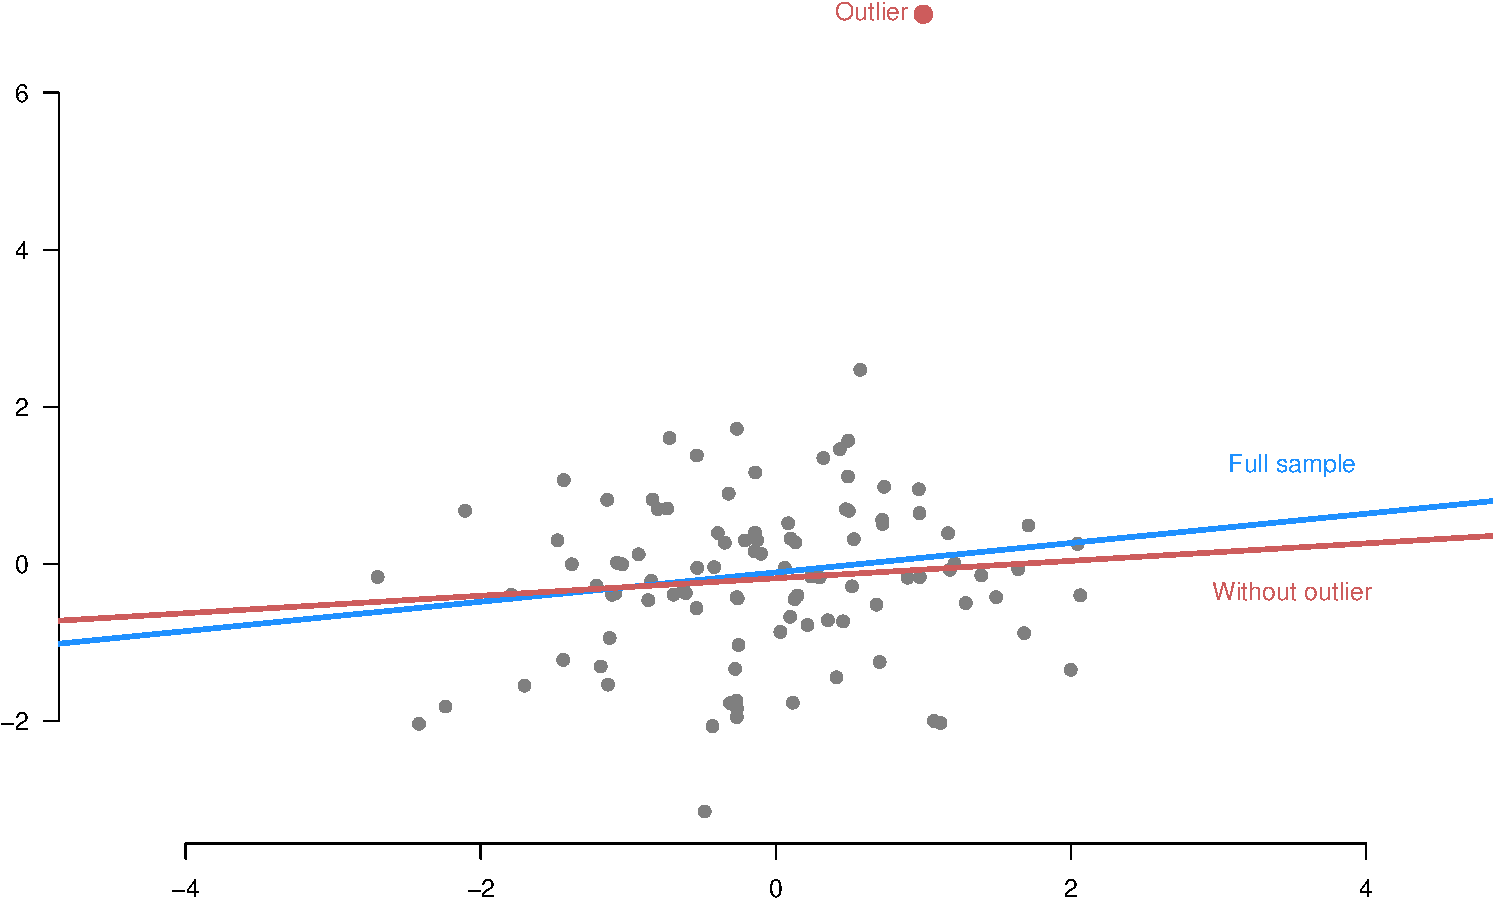
\includegraphics{least_squares_files/figure-pdf/fig-outlier-1.pdf}

}

\caption{\label{fig-outlier}An example of an outlier.}

\end{figure}%

Intuitively, it seems as though we could use the residual
\(\widehat{e}_i\) to assess the prediction error for a given unit. But
the residuals are not valid predictions because the OLS estimator is
designed to make those as small as possible (in machine learning
parlance, these were in the training set). In particular, if an outlier
is influential, we already noted that it might ``pull'' the regression
line toward it, and the resulting residual might be pretty small.

To assess prediction errors more cleanly, we can use
\textbf{leave-one-out regression} (LOO), which regresses
\(\mb{Y}_{(-i)}\) on \(\Xmat_{(-i)}\), where these omit unit \(i\): \[ 
\bhat_{(-i)} = \left(\Xmat'_{(-i)}\Xmat_{(-i)}\right)^{-1}\Xmat_{(-i)}\mb{Y}_{(-i)}.
\] We can then calculate LOO prediction errors as \[ 
\widetilde{e}_{i} = Y_{i} - \X_{i}'\bhat_{(-i)}.
\] Calculating these LOO prediction errors for each unit appears to be
computationally costly because it seems as though we have to fit OLS
\(n\) times. Fortunately, there is a closed-form expression for the LOO
coefficients and prediction errors in terms of the original regression,
\begin{equation}\phantomsection\label{eq-loo-coefs}{ 
\bhat_{(-i)} = \bhat - \left( \Xmat'\Xmat\right)^{-1}\X_i\widetilde{e}_i \qquad \widetilde{e}_i = \frac{\widehat{e}_i}{1 - h_{ii}}.
}\end{equation} This shows that the LOO prediction errors will differ
from the residuals when the leverage of a unit is high. This makes
sense! We said earlier that observations with low leverage would be
close to \(\overline{\X}\), where the outcome values have relatively
little impact on the OLS fit (because the regression line must go
through \(\overline{Y}\)).

\subsection{Influential observations}\label{influential-observations}

An influential observation (also sometimes called an influential point)
is a unit that has the power to change the coefficients and fitted
values for a particular OLS specification. Figure~\ref{fig-influence}
shows an example of such an influence point.

\begin{figure}[th]

\centering{

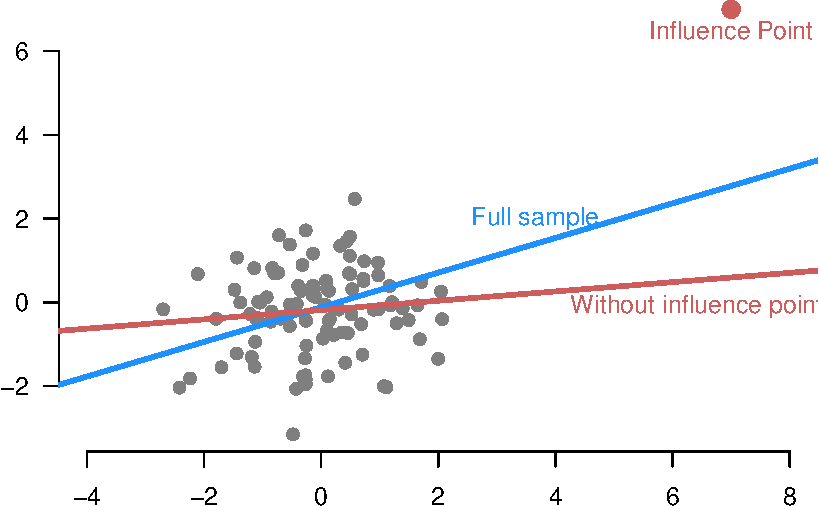
\includegraphics{least_squares_files/figure-pdf/fig-influence-1.pdf}

}

\caption{\label{fig-influence}An example of an influence point.}

\end{figure}%

One measure of influence, called DFBETA\(_i\), measures how much \(i\)
changes the estimated coefficient vector \[ 
\bhat - \bhat_{(-i)} = \left( \Xmat'\Xmat\right)^{-1}\X_i\widetilde{e}_i,
\] so there is one value for each observation-covariate pair. When
divided by the standard error of the estimated coefficients, this is
called DFBETA\textbf{S} (where the ``S'' is for standardized). These are
helpful if we focus on a particular coefficient.

When we want to summarize how much an observation matters for the fit,
we can use a compact measure of the influence of an observation by
comparing the fitted value from the entire sample to the fitted value
from the leave-one-out regression. Using the DFBETA above, we have \[ 
\widehat{Y}_i - \X_{i}\bhat_{(-1)} = \X_{i}'(\bhat -\bhat_{(-1)}) = \X_{i}'\left( \Xmat'\Xmat\right)^{-1}\X_i\widetilde{e}_i = h_{ii}\widetilde{e}_i,
\] so the influence of an observation is its leverage multiplied by how
much of an outlier it is. This value is sometimes called DFFIT
(difference in fit). One transformation of this quantity, \textbf{Cook's
distance}, standardizes this by the sum of the squared residuals: \[ 
D_i = \frac{n-k-1}{k+1}\frac{h_{ii}\widetilde{e}_{i}^{2}}{\widehat{\mb{e}}'\widehat{\mb{e}}}.
\] Different cutoffs exist for identifying ``influential'' observations,
but they tend to be ad hoc. In any case, the more important question is
``how much does this observation matter for my substantive
interpretation'' rather than the narrow question of a particular
threshold.

It's all well and good to find influential observations, but what should
be done about them? The first thing to check is that the data is not
corrupted somehow. Influence points sometimes occur because of a coding
or data entry error. We may consider removing the observation if the
error appears in the data acquired from another source but exercise
transparency if this appears to be the case. Another approach is to
consider a transformation of the dependent or independent variables,
like taking the natural logarithm, that might dampen the effects of
outliers. Finally, consider using methods that are robust to outliers
such as least absolute deviations or least trimmed squares.

\section{Summary}\label{summary-5}

In this chapter, we introduced the \textbf{ordinary least squares}
estimator, which finds the linear function of the \(\X_i\) that
minimizes the sum of the squared residuals and is the sample version of
the best linear predictor in the last chapter. The \(R^2\) statistic
assesses the in-sample \textbf{model fit} of OLS by comparing how much
better it predicts the outcome compared to a simple baseline predictor
of the sample mean of the outcome. OLS can also be written in a very
compact manner using matrix algebra, which allows us to understand the
geometry of OLS as a \textbf{projection} of the outcome into space of
linear functions of the independent variables. The
\textbf{Frisch-Waugh-Lovell theorem} describes a residual regression
approach to obtaining OLS estimates for subsets of coefficients, which
can be helpful for computational efficiency or data visualization.
Lastly, influential observations are those that alter the estimated
coefficients when they are omitted from the OLS estimation, and there
are several metrics that help to assess this. In the next chapter, we
move from the mechanical properties to the statistical properties of
OLS: unbiasedness, consistency, and asymptotic normality.

\chapter{The statistics of least squares}\label{sec-ols-statistics}

The last chapter showcased the least squares estimator and investigated
many of its more mechanical properties, which are essential for the
practical application of OLS. But we still need to understand its
statistical properties, as we discussed in Part I of this book:
unbiasedness, sampling variance, consistency, and asymptotic normality.
As we saw then, these properties fall into finite-sample (unbiasedness,
sampling variance) and asymptotic (consistency, asymptotic normality).

In this chapter, we will focus on the asymptotic properties of OLS
because those properties hold under the relatively mild conditions of
the linear projection model introduced in
Section~\ref{sec-linear-projection}. We will see that OLS consistently
estimates a coherent quantity of interest (the best linear predictor)
regardless of whether the conditional expectation is linear. That is,
for the asymptotic properties of the estimator, we will not need the
commonly invoked linearity assumption. Later, when we investigate the
finite-sample properties, we will show how linearity will help us
establish unbiasedness and also how the normality of the errors can
allow us to conduct exact, finite-sample inference. But these
assumptions are very strong, so understanding what we can say about OLS
without them is vital.

\section{Large-sample properties of
OLS}\label{large-sample-properties-of-ols}

As we saw in Chapter~\ref{sec-asymptotics}, we need two key ingredients
to conduct statistical inference with the OLS estimator: (1) a
consistent estimate of the variance of \(\bhat\) and (2) the approximate
distribution of \(\bhat\) in large samples. Remember that, since
\(\bhat\) is a vector, the variance of that estimator will actually be a
variance-covariance matrix. To obtain the two key ingredients, we first
establish the consistency of OLS and then use the central limit theorem
to derive its asymptotic distribution, which includes its variance.

We begin by setting out the assumptions needed for establishing the
large-sample properties of OLS, which are the same as the assumptions
needed to ensure that the best linear predictor,
\(\bhat = \E[\X_{i}\X_{i}']^{-1}\E[\X_{i}Y_{i}]\), is well-defined and
unique.

\begin{tcolorbox}[enhanced jigsaw, toptitle=1mm, bottomrule=.15mm, leftrule=.75mm, rightrule=.15mm, breakable, colframe=quarto-callout-note-color-frame, title=\textcolor{quarto-callout-note-color}{\faInfo}\hspace{0.5em}{Linear projection assumptions}, colbacktitle=quarto-callout-note-color!10!white, titlerule=0mm, coltitle=black, left=2mm, colback=white, bottomtitle=1mm, opacitybacktitle=0.6, opacityback=0, toprule=.15mm, arc=.35mm]

The linear projection model makes the following assumptions:

\begin{enumerate}
\def\labelenumi{\arabic{enumi}.}
\item
  \(\{(Y_{i}, \X_{i})\}_{i=1}^n\) are iid random vectors
\item
  \(\E[Y^{2}_{i}] < \infty\) (finite outcome variance)
\item
  \(\E[\Vert \X_{i}\Vert^{2}] < \infty\) (finite variances and
  covariances of covariates)
\item
  \(\E[\X_{i}\X_{i}']\) is positive definite (no linear dependence in
  the covariates)
\end{enumerate}

\end{tcolorbox}

Recall that these are mild conditions on the joint distribution of
\((Y_{i}, \X_{i})\) and in particular, we are \textbf{not} assuming
linearity of the CEF, \(\E[Y_{i} \mid \X_{i}]\), nor are we assuming any
specific distribution for the data.

We can helpfully decompose the OLS estimator into the actual BLP
coefficient plus estimation error as \[ 
\bhat = \left( \frac{1}{n} \sum_{i=1}^n \X_i\X_i' \right)^{-1} \left( \frac{1}{n} \sum_{i=1}^n \X_iY_i \right) = \bfbeta + \underbrace{\left( \frac{1}{n} \sum_{i=1}^n \X_i\X_i' \right)^{-1} \left( \frac{1}{n} \sum_{i=1}^n \X_ie_i \right)}_{\text{estimation error}}.
\]

This decomposition will help us quickly establish the consistency of
\(\bhat\). By the law of large numbers, we know that sample means will
converge in probability to population expectations, so we have \[ 
\frac{1}{n} \sum_{i=1}^n \X_i\X_i' \inprob \E[\X_i\X_i'] \equiv \mb{Q}_{\X\X} \qquad \frac{1}{n} \sum_{i=1}^n \X_ie_i \inprob \E[\X_{i} e_{i}] = \mb{0},
\] which implies by the continuous mapping theorem (the inverse is a
continuous function) that \[
\bhat \inprob \bfbeta + \mb{Q}_{\X\X}^{-1}\E[\X_ie_i] = \bfbeta,
\] The linear projection assumptions ensure that the LLN applies to
these sample means and that \(\E[\X_{i}\X_{i}']\) is invertible.

\begin{theorem}[]\protect\hypertarget{thm-ols-consistency}{}\label{thm-ols-consistency}

Under the above linear projection assumptions, the OLS estimator is
consistent for the best linear projection coefficients,
\(\bhat \inprob \bfbeta\).

\end{theorem}

Thus, OLS should be close to the population linear regression in large
samples under relatively mild conditions. Remember that this may not
equal the conditional expectation if the CEF is nonlinear. What we can
say is that OLS converges to the best \emph{linear} approximation to the
CEF. Of course, this also means that, if the CEF is linear, then OLS
will consistently estimate the coefficients of the CEF.

To emphasize, the only assumptions made about the dependent variable are
that it (1) has finite variance and (2) is iid. Under this assumption,
the outcome could be continuous, categorical, binary, or event count.

Next, we would like to establish an asymptotic normality result for the
OLS coefficients. We first review some key ideas about the Central Limit
Theorem.

\begin{tcolorbox}[enhanced jigsaw, toptitle=1mm, bottomrule=.15mm, leftrule=.75mm, rightrule=.15mm, breakable, colframe=quarto-callout-note-color-frame, title=\textcolor{quarto-callout-note-color}{\faInfo}\hspace{0.5em}{CLT reminder}, colbacktitle=quarto-callout-note-color!10!white, titlerule=0mm, coltitle=black, left=2mm, colback=white, bottomtitle=1mm, opacitybacktitle=0.6, opacityback=0, toprule=.15mm, arc=.35mm]

Suppose that we have a function of the data iid random vectors
\(\X_1, \ldots, \X_n\), \(g(\X_{i})\) where \(\E[g(\X_{i})] = 0\) and so
\(\V[g(\X_{i})] = \E[g(\X_{i})g(\X_{i})']\). Then if
\(\E[\Vert g(\X_{i})\Vert^{2}] < \infty\), the CLT implies that
\begin{equation}\phantomsection\label{eq-clt-mean-zero}{ 
\sqrt{n}\left(\frac{1}{n} \sum_{i=1}^{n} g(\X_{i}) - \E[g(\X_{i})]\right) = \frac{1}{\sqrt{n}} \sum_{i=1}^{n} g(\X_{i}) \indist \N(0, \E[g(\X_{i})g(\X_{i}')]) 
}\end{equation}

\end{tcolorbox}

We now manipulate our decomposition to arrive at the \emph{stabilized}
version of the estimator, \[ 
\sqrt{n}\left( \bhat - \bfbeta\right) = \left( \frac{1}{n} \sum_{i=1}^n \X_i\X_i' \right)^{-1} \left( \frac{1}{\sqrt{n}} \sum_{i=1}^n \X_ie_i \right).
\] Recall that we stabilize an estimator to ensure it has a fixed
variance as the sample size grows, allowing it to have a non-degenerate
asymptotic distribution. The stabilization works by asymptotically
centering it (that is, subtracting the value to which it converges) and
multiplying by the square root of the sample size. We have already
established that the first term on the right-hand side will converge in
probability to \(\mb{Q}_{\X\X}^{-1}\). Notice that
\(\E[\X_{i}e_{i}] = 0\), so we can apply Equation~\ref{eq-clt-mean-zero}
to the second term. The covariance matrix of \(\X_ie_{i}\) is \[ 
\mb{\Omega} = \V[\X_{i}e_{i}] = \E[\X_{i}e_{i}(\X_{i}e_{i})'] = \E[e_{i}^{2}\X_{i}\X_{i}'].
\] The CLT will imply that \[ 
\frac{1}{\sqrt{n}} \sum_{i=1}^n \X_ie_i \indist \N(0, \mb{\Omega}).
\] Combining these facts with Slutsky's Theorem implies the following
theorem.

\begin{theorem}[]\protect\hypertarget{thm-ols-asymptotic-normality}{}\label{thm-ols-asymptotic-normality}

Suppose that the linear projection assumptions hold and, in addition, we
have \(\E[Y_{i}^{4}] < \infty\) and
\(\E[\lVert\X_{i}\rVert^{4}] < \infty\). Then the OLS estimator is
asymptotically normal with \[ 
\sqrt{n}\left( \bhat - \bfbeta\right) \indist \N(0, \mb{V}_{\bfbeta}),
\] where \[ 
\mb{V}_{\bfbeta} = \mb{Q}_{\X\X}^{-1}\mb{\Omega}\mb{Q}_{\X\X}^{-1} = \left( \E[\X_i\X_i'] \right)^{-1}\E[e_i^2\X_i\X_i']\left( \E[\X_i\X_i'] \right)^{-1}.
\]

\end{theorem}

Thus, with a large enough sample size we can approximate the
distribution of \(\bhat\) with a multivariate normal distribution with
mean \(\bfbeta\) and covariance matrix \(\mb{V}_{\bfbeta}/n\). In
particular, the square root of the \(j\)th diagonals of this matrix will
be standard errors for \(\widehat{\beta}_j\). Knowing the shape of the
OLS estimator's multivariate distribution will allow us to conduct
hypothesis tests and generate confidence intervals for both individual
coefficients and groups of coefficients. But, first, we need an estimate
of the covariance matrix.

\section{Variance estimation for OLS}\label{variance-estimation-for-ols}

The asymptotic normality of OLS from the last section is of limited
value without some way to estimate the covariance matrix, \[ 
\mb{V}_{\bfbeta} = \mb{Q}_{\X\X}^{-1}\mb{\Omega}\mb{Q}_{\X\X}^{-1}.
\] Since each term here is a population mean, this is an ideal place in
which to drop a plug-in estimator. For now, we will use the following
estimators: \[ 
\begin{aligned}
  \mb{Q}_{\X\X} &= \E[\X_{i}\X_{i}'] & \widehat{\mb{Q}}_{\X\X} &= \frac{1}{n} \sum_{i=1}^{n} \X_{i}\X_{i}' = \frac{1}{n}\Xmat'\Xmat \\
  \mb{\Omega} &= \E[e_i^2\X_i\X_i'] & \widehat{\mb{\Omega}} & = \frac{1}{n}\sum_{i=1}^n\widehat{e}_i^2\X_i\X_i'.
\end{aligned}
\] Under the assumptions of Theorem~\ref{thm-ols-asymptotic-normality},
the LLN will imply that these are consistent for the quantities we need,
\(\widehat{\mb{Q}}_{\X\X} \inprob \mb{Q}_{\X\X}\) and
\(\widehat{\mb{\Omega}} \inprob \mb{\Omega}\). We can plug these into
the variance formula to arrive at \[ 
\begin{aligned}
  \widehat{\mb{V}}_{\bfbeta} &= \widehat{\mb{Q}}_{\X\X}^{-1}\widehat{\mb{\Omega}}\widehat{\mb{Q}}_{\X\X}^{-1} \\
  &= \left( \frac{1}{n} \Xmat'\Xmat \right)^{-1} \left( \frac{1}{n} \sum_{i=1}^n\widehat{e}_i^2\X_i\X_i' \right) \left( \frac{1}{n} \Xmat'\Xmat \right)^{-1},
\end{aligned}
\] which by the continuous mapping theorem is consistent,
\(\widehat{\mb{V}}_{\bfbeta} \inprob \mb{V}_{\bfbeta}\).

This estimator is sometimes called the \textbf{robust variance
estimator} or, more accurately, the
\textbf{heteroskedasticity-consistent (HC) variance estimator}. Why is
it robust? Consider the standard \textbf{homoskedasticity} assumption
that most statistical software packages make when estimating OLS
variances: the variance of the errors does not depend on the covariates,
or \(\V[e_{i}^{2} \mid \X_{i}] = \V[e_{i}^{2}]\). This assumption is
stronger than needed, and we can rely on a weaker assumption that the
squared errors are uncorrelated with a specific function of the
covariates: \[ 
\E[e_{i}^{2}\X_{i}\X_{i}'] = \E[e_{i}^{2}]\E[\X_{i}\X_{i}'] = \sigma^{2}\mb{Q}_{\X\X}, 
\] where \(\sigma^2\) is the variance of the residuals (since
\(\E[e_{i}] = 0\)). Homoskedasticity simplifies the asymptotic variance
of the stabilized estimator, \(\sqrt{n}(\bhat - \bfbeta)\), to \[ 
\mb{V}^{\texttt{lm}}_{\bfbeta} = \mb{Q}_{\X\X}^{-1}\sigma^{2}\mb{Q}_{\X\X}\mb{Q}_{\X\X}^{-1} = \sigma^2\mb{Q}_{\X\X}^{-1}.
\] We already have an estimator for \(\mb{Q}_{\X\X}\), but we need one
for \(\sigma^2\). We can easily use the SSR, \[ 
\widehat{\sigma}^{2} = \frac{1}{n-k-1} \sum_{i=1}^{n} \widehat{e}_{i}^{2},
\] where we use \(n-k-1\) in the denominator instead of \(n\) to correct
for the residuals being slightly less variable than the actual errors
(because OLS mechanically attempts to make the residuals small). For
consistent variance estimation, \(n-k -1\) or \(n\) can be used, since
either way \(\widehat{\sigma}^2 \inprob \sigma^2\). Thus, under
homoskedasticity, we have \[ 
\widehat{\mb{V}}_{\bfbeta}^{\texttt{lm}} = \widehat{\sigma}^{2}\left(\Xmat'\Xmat\right)^{{-1}},
\] This is the standard variance estimator used by \texttt{lm()} in R
and \texttt{reg} in Stata.

How do these two estimators, \(\widehat{\mb{V}}_{\bfbeta}\) and
\(\widehat{\mb{V}}_{\bfbeta}^{\texttt{lm}}\), compare? Notice that the
HC variance estimator and the homoskedasticity variance estimator will
both be consistent when homoskedasticity holds. But as the
``heteroskedasticity-consistent'' label implies, only the HC variance
estimator will be consistent when homoskedasticity fails to hold. So
\(\widehat{\mb{V}}_{\bfbeta}\) has the advantage of being consistent
regardless of the homoskedasticity assumption. This advantage comes at a
cost, however. When homoskedasticity is correct,
\(\widehat{\mb{V}}_{\bfbeta}^{\texttt{lm}}\) incorporates that
assumption into the estimator whereas the HC variance estimator has to
estimate it. The HC estimator will therefore have higher variance (the
variance estimator will be more variable!) when homoskedasticity
actually does hold.

Now that we have established the asymptotic normality of the OLS
estimator and developed a consistent estimator of its variance, we can
proceed with all of the statistical inference tools we discussed in Part
I, including hypothesis tests and confidence intervals.

We begin by defining the estimated \textbf{heteroskedasticity-consistent
standard errors} as \[ 
\widehat{\se}(\widehat{\beta}_{j}) = \sqrt{\frac{[\widehat{\mb{V}}_{\bfbeta}]_{jj}}{n}},
\] where \([\widehat{\mb{V}}_{\bfbeta}]_{jj}\) is the \(j\)th diagonal
entry of the HC variance estimator. Note that we divide by \(\sqrt{n}\)
here because \(\widehat{\mb{V}}_{\bfbeta}\) is a consistent estimator of
the stabilized estimator \(\sqrt{n}(\bhat - \bfbeta)\) not the estimator
itself.

Hypothesis tests and confidence intervals for individual coefficients
are almost precisely the same as with the most general case presented in
Part I. For a two-sided test of \(H_0: \beta_j = b\) versus
\(H_1: \beta_j \neq b\), we can build the t-statistic and conclude that,
under the null, \[
\frac{\widehat{\beta}_j - b}{\widehat{\se}(\widehat{\beta}_{j})} \indist \N(0, 1).
\] Statistical software will typically and helpfully provide the
t-statistic for the null hypothesis of no (partial) linear relationship
between \(X_{ij}\) and \(Y_i\), \[ 
t = \frac{\widehat{\beta}_{j}}{\widehat{\se}(\widehat{\beta}_{j})},
\] which measures how large the estimated coefficient is in standard
errors. With \(\alpha = 0.05\), asymptotic normality would imply that we
reject this null when \(t > 1.96\). We can form asymptotically-valid
confidence intervals with \[ 
\left[\widehat{\beta}_{j} - z_{\alpha/2}\;\widehat{\se}(\widehat{\beta}_{j}),\;\widehat{\beta}_{j} + z_{\alpha/2}\;\widehat{\se}(\widehat{\beta}_{j})\right]. 
\] For reasons we will discuss below, standard software typically relies
on the \(t\) distribution instead of the normal for hypothesis testing
and confidence intervals. Still, this difference is of little
consequence in large samples.

\section{Inference for multiple
parameters}\label{inference-for-multiple-parameters}

With multiple coefficients, we might have hypotheses that involve more
than one coefficient. As an example, consider a regression with an
interaction between two covariates, \[
Y_i = \beta_0 + X_i\beta_1 + Z_i\beta_2 + X_iZ_i\beta_3 + e_i.
\] Suppose we wanted to test the hypothesis that \(X_i\) does not affect
the best linear predictor for \(Y_i\). That would be \[ 
H_{0}: \beta_{1} = 0 \text{ and } \beta_{3} = 0\quad\text{vs}\quad H_{1}: \beta_{1} \neq 0 \text{ or } \beta_{3} \neq 0,
\] where we usually write the null more compactly as
\(H_0: \beta_1 = \beta_3 = 0\).

To test this null hypothesis, we need a test statistic that
discriminates between the two hypotheses: it should be large when the
alternative is true and small enough when the null is true. With a
single coefficient, we usually test the null hypothesis of
\(H_0: \beta_j = b_0\) with the \(t\)-statistic, \[ 
t = \frac{\widehat{\beta}_{j} - b_{0}}{\widehat{\se}(\widehat{\beta}_{j})},
\] and we usually take the absolute value, \(|t|\), as our measure of
how extreme our estimate is given the null distribution. But notice that
we could also use the square of the \(t\) statistic, which is
\begin{equation}\phantomsection\label{eq-squared-t}{ 
t^{2} = \frac{\left(\widehat{\beta}_{j} - b_{0}\right)^{2}}{\V[\widehat{\beta}_{j}]} = \frac{n\left(\widehat{\beta}_{j} - b_{0}\right)^{2}}{[\mb{V}_{\bfbeta}]_{[jj]}}. 
}\end{equation}

While \(|t|\) is the usual test statistic we use for two-sided tests, we
could equivalently use \(t^2\) and arrive at the exact same conclusions
(as long as we knew the distribution of \(t^2\) under the null
hypothesis). It turns out that the \(t^2\) version of the test statistic
will generalize more easily to comparing multiple coefficients. This
version of the test statistic suggests another general way to
differentiate the null from the alternative: by taking the squared
distance between them and dividing by the variance of the estimate.

Can we generalize this idea to hypotheses about multiple parameters?
Adding the sum of squared distances for each component of the null
hypothesis is straightforward. For our interaction example, that would
be \[ 
\widehat{\beta}_1^2 + \widehat{\beta}_3^2, 
\] Remember, however, that some of the estimated coefficients are
noisier than others, so we should account for the uncertainty just like
we did for the \(t\)-statistic.

With multiple parameters and multiple coefficients, the variances will
now require matrix algebra. We can write any hypothesis about linear
functions of the coefficients as \(H_{0}: \mb{L}\bfbeta = \mb{c}\). For
example, in the interaction case, we have \[ 
\mb{L} =
\begin{pmatrix}
  0 & 1 & 0 & 0 \\
  0 & 0 & 0 & 1 \\
\end{pmatrix}
\qquad
\mb{c} =
\begin{pmatrix}
  0 \\
  0
\end{pmatrix}
\] Thus, \(\mb{L}\bfbeta = \mb{0}\) is equivalent to \(\beta_1 = 0\) and
\(\beta_3 = 0\). Notice that with other \(\mb{L}\) matrices, we could
represent more complicated hypotheses like \(2\beta_1 - \beta_2 = 34\),
though we mostly stick to simpler functions. Let
\(\widehat{\bs{\theta}} = \mb{L}\bhat\) be the OLS estimate of the
function of the coefficients. By the delta method (discussed in
Section~\ref{sec-delta-method}), we have \[ 
\sqrt{n}\left(\mb{L}\bhat - \mb{L}\bfbeta\right) \indist \N(0, \mb{L}'\mb{V}_{\bfbeta}\mb{L}).
\] We can now generalize the squared \(t\) statistic in
Equation~\ref{eq-squared-t} by taking the distances
\(\mb{L}\bhat - \mb{c}\) weighted by the variance-covariance matrix
\(\mb{L}'\mb{V}_{\bfbeta}\mb{L}\), \[ 
W = n(\mb{L}\bhat - \mb{c})'(\mb{L}'\mb{V}_{\bfbeta}\mb{L})^{-1}(\mb{L}\bhat - \mb{c}),
\] which is called the \textbf{Wald test statistic}. This statistic
generalizes the ideas of the t-statistic to multiple parameters. With
the t-statistic, we recenter to have mean 0 and divide by the standard
error to get a variance of 1. If we ignore the middle variance
weighting, we have \((\mb{L}\bhat - \mb{c})'(\mb{L}\bhat - \mb{c})\)
which is just the sum of the squared deviations of the estimates from
the null. Including the \((\mb{L}'\mb{V}_{\bfbeta}\mb{L})^{-1}\) weight
has the effect of rescaling the distribution of \(\mb{L}\bhat - \mb{c}\)
to make it rotationally symmetric around 0 (so the resulting dimensions
are uncorrelated) with each dimension having an equal variance of 1. In
this way, the Wald statistic transforms the random vectors to be
mean-centered and have variance 1 (just the t-statistic), but also to
have the resulting random variables in the vector be
uncorrelated.\footnote{The form of the Wald statistic is that of a
  weighted inner product, \(\mb{x}'\mb{Ay}\), where \(\mb{A}\) is a
  symmetric positive-definite weighting matrix.}

Why transform the data in this way? Figure~\ref{fig-wald} shows the
contour plot of a hypothetical joint distribution of two coefficients
from an OLS regression. We might want to know the distance between
different points in the distribution and the mean, which in this case is
\((1, 2)\). Without considering the joint distribution, the circle is
obviously closer to the mean than the triangle. However, looking at the
two points on the distribution, the circle is at a lower contour than
the triangle, meaning it is more extreme than the triangle for this
particular distribution. The Wald statistic, then, takes into
consideration how much of a ``climb'' it is for \(\mb{L}\bhat\) to get
to \(\mb{c}\) given the distribution of \(\mb{L}\bhat\).

\begin{figure}[th]

\centering{

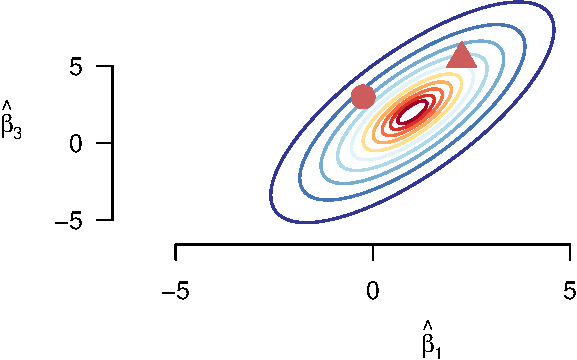
\includegraphics{ols_properties_files/figure-pdf/fig-wald-1.pdf}

}

\caption{\label{fig-wald}Hypothetical joint distribution of two slope
coefficients. The circle is closer to the center of the distribution by
the standard Euclidean distance, but the triangle is closer once you
consider the joint distribution.}

\end{figure}%

If \(\mb{L}\) only has one row, our Wald statistic is the same as the
squared \(t\) statistic, \(W = t^2\). This fact will help us think about
the asymptotic distribution of \(W\). Note that as \(n\to\infty\), we
know that by the asymptotic normality of \(\bhat\), \[ 
t = \frac{\widehat{\beta}_{j} - \beta_{j}}{\widehat{\se}[\widehat{\beta}_{j}]} \indist \N(0,1)
\] so \(t^2\) will converge in distribution to a \(\chi^2_1\) (since a
\(\chi^2_1\) distribution is just one standard normal distribution
squared). After recentering and rescaling by the covariance matrix,
\(W\) converges to the sum of \(q\) squared independent normals, where
\(q\) is the number of rows of \(\mb{L}\), or equivalently, the number
of restrictions implied by the null hypothesis. Thus, under the null
hypothesis of \(\mb{L}\bhat = \mb{c}\), we have
\(W \indist \chi^2_{q}\).

We need to define the rejection region to use the Wald statistic in a
hypothesis test. Because we are squaring each distance in \(W \geq 0\),
larger values of \(W\) indicate more disagreement with the null in
either direction. Thus, for an \(\alpha\)-level test of the joint null,
we only need a one-sided rejection region of the form
\(\P(W > w_{\alpha}) = \alpha\). Obtaining these values is
straightforward (see the above callout tip). For \(q = 2\) and a
\(\alpha = 0.05\), the critical value is roughly 6.

\begin{tcolorbox}[enhanced jigsaw, toptitle=1mm, bottomrule=.15mm, leftrule=.75mm, rightrule=.15mm, breakable, colframe=quarto-callout-note-color-frame, title=\textcolor{quarto-callout-note-color}{\faInfo}\hspace{0.5em}{Chi-squared critical values}, colbacktitle=quarto-callout-note-color!10!white, titlerule=0mm, coltitle=black, left=2mm, colback=white, bottomtitle=1mm, opacitybacktitle=0.6, opacityback=0, toprule=.15mm, arc=.35mm]

We can obtain critical values for the \(\chi^2_q\) distribution using
the \texttt{qchisq()} function in R. For example, if we wanted to obtain
the critical value \(w\) such that \(\P(W > w_{\alpha}) = \alpha\) for
our two-parameter interaction example, we could use:

\begin{Shaded}
\begin{Highlighting}[]
\FunctionTok{qchisq}\NormalTok{(}\AttributeTok{p =} \FloatTok{0.95}\NormalTok{, }\AttributeTok{df =} \DecValTok{2}\NormalTok{)}
\end{Highlighting}
\end{Shaded}

\begin{verbatim}
[1] 5.991465
\end{verbatim}

\end{tcolorbox}

The Wald statistic is not a common test provided by standard statistical
software functions like \texttt{lm()} in R, though it is fairly
straightforward to implement ``by hand.'' Alternatively, packages like
\href{https://cran.r-project.org/web/packages/aod/index.html}{\texttt{\{aod\}}}
or
\href{http://jepusto.github.io/clubSandwich/}{\texttt{\{clubSandwich\}}}
have implementations of the test. What is reported by most software
implementations of OLS (like \texttt{lm()} in R) is the F-statistic,
which is \[ 
F = \frac{W}{q}.
\] This also typically uses the homoskedastic variance estimator
\(\mb{V}^{\texttt{lm}}_{\bfbeta}\) in \(W\). The p-values reported for
such tests use the \(F_{q,n-k-1}\) distribution because this is the
exact distribution of the \(F\) statistic when the errors are (a)
homoskedastic and (b) normally distributed. When these assumptions do
not hold, the \(F\) distribution has no justification in statistical
theory, but it is slightly more conservative than the \(\chi^2_q\)
distribution, and the inferences from the \(F\) statistic will converge
to those from the \(\chi^2_q\) distribution as \(n\to\infty\). So it
might be justified as an \emph{ad hoc} small-sample adjustment to the
Wald test. For example, if we used the \(F_{q,n-k-1}\) with the
interaction example where \(q=2\) and we have, say, a sample size of
\(n = 100\), then in that case, the critical value for the F test with
\(\alpha = 0.05\) is

\begin{Shaded}
\begin{Highlighting}[]
\FunctionTok{qf}\NormalTok{(}\FloatTok{0.95}\NormalTok{, }\AttributeTok{df1 =} \DecValTok{2}\NormalTok{, }\AttributeTok{df2 =} \DecValTok{100} \SpecialCharTok{{-}} \DecValTok{4}\NormalTok{)}
\end{Highlighting}
\end{Shaded}

\begin{verbatim}
[1] 3.091191
\end{verbatim}

This result implies a critical value of 6.182 on the scale of the Wald
statistic (multiplying it by \(q = 2\)). Compared to the earlier
critical value of 5.991 based on the \(\chi^2_2\) distribution, we can
see that the inferences will be very similar even in moderately-sized
datasets.

Finally, note that the F-statistic reported by \texttt{lm()} in R is the
test of all the coefficients being equal to 0 jointly except for the
intercept. In modern quantitative social sciences, this test is seldom
substantively interesting.

\section{Finite-sample properties with a linear
CEF}\label{finite-sample-properties-with-a-linear-cef}

All the above results have been large-sample properties, and we have not
addressed finite-sample properties like the sampling variance or
unbiasedness. Under the linear projection assumption above, OLS is
generally biased without stronger assumptions. This section introduces
the stronger assumption that will allow us to establish stronger
properties for OLS. As usual, however, remember that these stronger
assumptions can be wrong.

\begin{tcolorbox}[enhanced jigsaw, toptitle=1mm, bottomrule=.15mm, leftrule=.75mm, rightrule=.15mm, breakable, colframe=quarto-callout-note-color-frame, title=\textcolor{quarto-callout-note-color}{\faInfo}\hspace{0.5em}{Assumption: Linear Regression Model}, colbacktitle=quarto-callout-note-color!10!white, titlerule=0mm, coltitle=black, left=2mm, colback=white, bottomtitle=1mm, opacitybacktitle=0.6, opacityback=0, toprule=.15mm, arc=.35mm]

\begin{enumerate}
\def\labelenumi{\arabic{enumi}.}
\item
  The variables \((Y_{i}, \X_{i})\) satisfy the linear CEF assumption.
  \[ 
  \begin{aligned}
    Y_{i} &= \X_{i}'\bfbeta + e_{i} \\
    \E[e_{i}\mid \X_{i}] & = 0.
  \end{aligned}
  \]
\item
  The design matrix is invertible \(\E[\X_{i}\X_{i}'] > 0\) (positive
  definite).
\end{enumerate}

\end{tcolorbox}

We discussed the concept of a linear CEF extensively in
Chapter~\ref{sec-regression}. However, recall that the CEF might be
linear mechanically if the model is \textbf{saturated} or when there are
as many coefficients in the model as there are unique values of
\(\X_i\). When a model is not saturated, the linear CEF assumption is
just that: an assumption. What can this assumption do? It can aid in
establishing some nice statistical properties in finite samples.

Before proceeding, note that, when focusing on the finite sample
inference for OLS, we focused on its properties \textbf{conditional on
the observed covariates}, such as \(\E[\bhat \mid \Xmat]\) or
\(\V[\bhat \mid \Xmat]\). The historical reason for this is that the
researcher often chose these independent variables and so they were not
random. Thus, sometimes \(\Xmat\) is treated as ``fixed'' in some older
texts, which might even omit explicit conditioning statements.

\begin{theorem}[]\protect\hypertarget{thm-ols-unbiased}{}\label{thm-ols-unbiased}

Under the linear regression model assumption, OLS is unbiased for the
population regression coefficients, \[
\E[\bhat \mid \Xmat] = \bfbeta,
\] and its conditional sampling variance is \[
\mb{\V}_{\bhat} = \V[\bhat \mid \Xmat] = \left( \Xmat'\Xmat \right)^{-1}\left( \sum_{i=1}^n \sigma^2_i \X_i\X_i' \right) \left( \Xmat'\Xmat \right)^{-1},
\] where \(\sigma^2_{i} = \E[e_{i}^{2} \mid \Xmat]\).

\end{theorem}

\begin{proof}
To prove the conditional unbiasedness, recall that we can write the OLS
estimator as \[
\bhat = \bfbeta + (\Xmat'\Xmat)^{-1}\Xmat'\mb{e},
\] and so taking (conditional) expectations, we have \[
\E[\bhat \mid \Xmat] = \bfbeta + \E[(\Xmat'\Xmat)^{-1}\Xmat'\mb{e} \mid \Xmat] = \bfbeta + (\Xmat'\Xmat)^{-1}\Xmat'\E[\mb{e} \mid \Xmat] = \bfbeta,
\] because under the linear CEF assumption \(\E[\mb{e}\mid \Xmat] = 0\).

For the conditional sampling variance, we can use the same decomposition
we have, \[
\V[\bhat \mid \Xmat] = \V[\bfbeta + (\Xmat'\Xmat)^{-1}\Xmat'\mb{e} \mid \Xmat] = (\Xmat'\Xmat)^{-1}\Xmat'\V[\mb{e} \mid \Xmat]\Xmat(\Xmat'\Xmat)^{-1}. 
\] Since \(\E[\mb{e}\mid \Xmat] = 0\), we know that
\(\V[\mb{e}\mid \Xmat] = \E[\mb{ee}' \mid \Xmat]\), which is a matrix
with diagonal entries \(\E[e_{i}^{2} \mid \Xmat] = \sigma^2_i\) and
off-diagonal entries
\(\E[e_{i}e_{j} \Xmat] = \E[e_{i}\mid \Xmat]\E[e_{j}\mid\Xmat] = 0\),
where the first equality follows from the independence of the errors
across units. Thus, \(\V[\mb{e} \mid \Xmat]\) is a diagonal matrix with
\(\sigma^2_i\) along the diagonal, which means \[
\Xmat'\V[\mb{e} \mid \Xmat]\Xmat = \sum_{i=1}^n \sigma^2_i \X_i\X_i',
\] establishing the conditional sampling variance.
\end{proof}

This means that, for any realization of the covariates, \(\Xmat\), OLS
is unbiased for the true regression coefficients \(\bfbeta\). By the law
of iterated expectation, we also know that it is unconditionally
unbiased\footnote{We are basically ignoring some edge cases when it
  comes to discrete covariates here. In particular, we assume that
  \(\Xmat'\Xmat\) is nonsingular with probability one. However, this
  assumption can fail if we have a binary covariate since there is some
  chance (however slight) that the entire column will be all ones or all
  zeros, which would lead to a singular matrix \(\Xmat'\Xmat\).
  Practically this is not a big deal, but it does mean that we have to
  ignore this issue theoretically or focus on conditional unbiasedness.}
as well since \[
\E[\bhat] = \E[\E[\bhat \mid \Xmat]] = \bfbeta. 
\] The difference between these two statements usually isn't incredibly
meaningful.

There are a lot of variances flying around, so reviewing them is
helpful. Above, we derived the asymptotic variance of
\(\mb{Z}_{n} = \sqrt{n}(\bhat - \bfbeta)\), \[
\mb{V}_{\bfbeta} = \left( \E[\X_i\X_i'] \right)^{-1}\E[e_i^2\X_i\X_i']\left( \E[\X_i\X_i'] \right)^{-1},
\] which implies that the approximate variance of \(\bhat\) will be
\(\mb{V}_{\bfbeta} / n\) because \[
\bhat = \frac{Z_n}{\sqrt{n}} + \bfbeta \quad\implies\quad \bhat \overset{a}{\sim} \N(\bfbeta, n^{-1}\mb{V}_{\bfbeta}),
\] where \(\overset{a}{\sim}\) means asymptotically distributed as.
Under the linear CEF, the conditional sampling variance of \(\bhat\) has
a similar form and will be similar to the\\
\[
\mb{V}_{\bhat} = \left( \Xmat'\Xmat \right)^{-1}\left( \sum_{i=1}^n \sigma^2_i \X_i\X_i' \right) \left( \Xmat'\Xmat \right)^{-1} \approx \mb{V}_{\bfbeta} / n.
\] In practice, these two derivations lead to basically the same
variance estimator. Recall that the heteroskedastic-consistent variance
estimator \[
\widehat{\mb{V}}_{\bfbeta} = \left( \frac{1}{n} \Xmat'\Xmat \right)^{-1} \left( \frac{1}{n} \sum_{i=1}^n\widehat{e}_i^2\X_i\X_i' \right) \left( \frac{1}{n} \Xmat'\Xmat \right)^{-1},
\] is a valid plug-in estimator for the asymptotic variance and \[
\widehat{\mb{V}}_{\bhat} = n^{-1}\widehat{\mb{V}}_{\bfbeta}.
\] Thus, in practice, the asymptotic and finite-sample results under a
linear CEF justify the same variance estimator.

\subsection{Linear CEF model under
homoskedasticity}\label{linear-cef-model-under-homoskedasticity}

If we are willing to assume that the standard errors are homoskedastic,
we can derive even stronger results for OLS. Stronger assumptions
typically lead to stronger conclusions, but, obviously, those
conclusions may not be robust to assumption violations. But
homoskedasticity of errors is such a historically important assumption
that statistical software implementations of OLS like \texttt{lm()} in R
assume it by default.

\begin{tcolorbox}[enhanced jigsaw, toptitle=1mm, bottomrule=.15mm, leftrule=.75mm, rightrule=.15mm, breakable, colframe=quarto-callout-note-color-frame, title=\textcolor{quarto-callout-note-color}{\faInfo}\hspace{0.5em}{Assumption: Homoskedasticity with a linear CEF}, colbacktitle=quarto-callout-note-color!10!white, titlerule=0mm, coltitle=black, left=2mm, colback=white, bottomtitle=1mm, opacitybacktitle=0.6, opacityback=0, toprule=.15mm, arc=.35mm]

In addition to the linear CEF assumption, we further assume that \[
\E[e_i^2 \mid \X_i] = \E[e_i^2] = \sigma^2,
\] or that variance of the errors does not depend on the covariates.

\end{tcolorbox}

\begin{theorem}[]\protect\hypertarget{thm-homoskedasticity}{}\label{thm-homoskedasticity}

Under a linear CEF model with homoskedastic errors, the conditional
sampling variance is \[
\mb{V}^{\texttt{lm}}_{\bhat} = \V[\bhat \mid \Xmat] = \sigma^2 \left( \Xmat'\Xmat \right)^{-1},
\] and the variance estimator \[
\widehat{\mb{V}}^{\texttt{lm}}_{\bhat} = \widehat{\sigma}^2 \left( \Xmat'\Xmat \right)^{-1} \quad\text{where,}\quad \widehat{\sigma}^2 = \frac{1}{n - k - 1} \sum_{i=1}^n \widehat{e}_i^2
\] is unbiased,
\(\E[\widehat{\mb{V}}^{\texttt{lm}}_{\bhat} \mid \Xmat] = \mb{V}^{\texttt{lm}}_{\bhat}\).

\end{theorem}

\begin{proof}
Under homoskedasticity \(\sigma^2_i = \sigma^2\) for all \(i\). Recall
that \(\sum_{i=1}^n \X_i\X_i' = \Xmat'\Xmat\). Thus, the conditional
sampling variance from Theorem~\ref{thm-ols-unbiased}, \[ 
\begin{aligned}
\V[\bhat \mid \Xmat] &= \left( \Xmat'\Xmat \right)^{-1}\left( \sum_{i=1}^n \sigma^2 \X_i\X_i' \right) \left( \Xmat'\Xmat \right)^{-1} \\ &= \sigma^2\left( \Xmat'\Xmat \right)^{-1}\left( \sum_{i=1}^n \X_i\X_i' \right) \left( \Xmat'\Xmat \right)^{-1} \\&= \sigma^2\left( \Xmat'\Xmat \right)^{-1}\left( \Xmat'\Xmat \right) \left( \Xmat'\Xmat \right)^{-1} \\&= \sigma^2\left( \Xmat'\Xmat \right)^{-1} = \mb{V}^{\texttt{lm}}_{\bhat}.
\end{aligned}
\]

For unbiasedness, we just need to show that
\(\E[\widehat{\sigma}^{2} \mid \Xmat] = \sigma^2\). Recall that we
defined \(\mb{M}_{\Xmat}\) as the residual-maker because
\(\mb{M}_{\Xmat}\mb{Y} = \widehat{\mb{e}}\). We can use this to connect
the residuals to the standard errors, \[ 
\mb{M}_{\Xmat}\mb{e} = \mb{M}_{\Xmat}\mb{Y} - \mb{M}_{\Xmat}\Xmat\bfbeta = \mb{M}_{\Xmat}\mb{Y} = \widehat{\mb{e}},
\] so \[
\V[\widehat{\mb{e}} \mid \Xmat] = \mb{M}_{\Xmat}\V[\mb{e} \mid \Xmat] = \mb{M}_{\Xmat}\sigma^2,
\] where the first equality holds because
\(\mb{M}_{\Xmat} = \mb{I}_{n} - \Xmat (\Xmat'\Xmat)^{-1} \Xmat'\) is
constant conditional on \(\Xmat\). Notice that the diagonal entries of
this matrix are the variances of particular residuals \(\widehat{e}_i\)
and that the diagonal entries of the annihilator matrix are
\(1 - h_{ii}\) (since the \(h_{ii}\) are the diagonal entries of
\(\mb{P}_{\Xmat}\)). Thus, we have \[ 
\V[\widehat{e}_i \mid \Xmat] = \E[\widehat{e}_{i}^{2} \mid \Xmat] = (1 - h_{ii})\sigma^{2}.
\] In the last chapter in Section~\ref{sec-leverage}, we established
that one property of these leverage values is
\(\sum_{i=1}^n h_{ii} = k+ 1\), so
\(\sum_{i=1}^n 1- h_{ii} = n - k - 1\) and we have \[ 
\begin{aligned}
  \E[\widehat{\sigma}^{2} \mid \Xmat] &= \frac{1}{n-k-1} \sum_{i=1}^{n} \E[\widehat{e}_{i}^{2} \mid \Xmat] \\
                                      &= \frac{\sigma^{2}}{n-k-1} \sum_{i=1}^{n} 1 - h_{ii} \\
                                      &= \sigma^{2}. 
\end{aligned}
\] This establishes
\(\E[\widehat{\mb{V}}^{\texttt{lm}}_{\bhat} \mid \Xmat] = \mb{V}^{\texttt{lm}}_{\bhat}\).
\end{proof}

Thus, under the linear CEF model and homoskedasticity of the errors, we
have an unbiased variance estimator that is a simple function of the sum
of squared residuals and the design matrix. Most statistical software
packages estimate standard errors using
\(\widehat{\mb{V}}^{\texttt{lm}}_{\bhat}\).

The final result we can derive for the linear CEF under the
homoskedasticity assumption is an optimality result. That is, we might
ask if there is another estimator for \(\bfbeta\) that would outperform
OLS in the sense of having a lower sampling variance. Perhaps
surprisingly, no linear estimator for \(\bfbeta\) has a lower
conditional variance, meaning that OLS is the \textbf{best linear
unbiased estimator}, often jovially shortened to BLUE. This result is
famously known as the Gauss-Markov Theorem.

\begin{theorem}[]\protect\hypertarget{thm-gauss-markov}{}\label{thm-gauss-markov}

Let \(\widetilde{\bfbeta} = \mb{AY}\) be a linear and unbiased estimator
for \(\bfbeta\). Under the linear CEF model with homoskedastic errors,
\[
\V[\widetilde{\bfbeta}\mid \Xmat] \geq \V[\bhat \mid \Xmat]. 
\]

\end{theorem}

\begin{proof}
Note that if \(\widetilde{\bfbeta}\) is unbiased then
\(\E[\widetilde{\bfbeta} \mid \Xmat] = \bfbeta\) and so \[
\bfbeta = \E[\mb{AY} \mid \Xmat] = \mb{A}\E[\mb{Y} \mid \Xmat] = \mb{A}\Xmat\bfbeta,
\] which implies that \(\mb{A}\Xmat = \mb{I}_n\). Rewrite the competitor
as \(\widetilde{\bfbeta} = \bhat + \mb{BY}\) where, \[ 
\mb{B} = \mb{A} - \left(\Xmat'\Xmat\right)^{-1}\Xmat'.
\] and note that \(\mb{A}\Xmat = \mb{I}_n\) implies that
\(\mb{B}\Xmat = 0\). We now have \[ 
\begin{aligned}
  \widetilde{\bfbeta} &= \left( \left(\Xmat'\Xmat\right)^{-1}\Xmat' + \mb{B}\right)\mb{Y} \\
                      &= \left( \left(\Xmat'\Xmat\right)^{-1}\Xmat' + \mb{B}\right)\Xmat\bfbeta + \left( \left(\Xmat'\Xmat\right)^{-1}\Xmat' + \mb{B}\right)\mb{e} \\
                      &= \bfbeta + \mb{B}\Xmat\bfbeta + \left( \left(\Xmat'\Xmat\right)^{-1}\Xmat' + \mb{B}\right)\mb{e} \\
  &= \bfbeta + \left( \left(\Xmat'\Xmat\right)^{-1}\Xmat' + \mb{B}\right)\mb{e}
\end{aligned}
\] The variance of the competitor is, thus, \[ 
\begin{aligned}
  \V[\widetilde{\bfbeta} \mid \Xmat]
  &= \left( \left(\Xmat'\Xmat\right)^{-1}\Xmat' + \mb{B}\right)\V[\mb{e}\mid \Xmat]\left( \left(\Xmat'\Xmat\right)^{-1}\Xmat' + \mb{B}\right)' \\
  &= \sigma^{2}\left( \left(\Xmat'\Xmat\right)^{-1}\Xmat' + \mb{B}\right)\left( \Xmat\left(\Xmat'\Xmat\right)^{-1} + \mb{B}'\right) \\
  &= \sigma^{2}\left(\left(\Xmat'\Xmat\right)^{-1}\Xmat'\Xmat\left(\Xmat'\Xmat\right)^{-1} + \left(\Xmat'\Xmat\right)^{-1}\Xmat'\mb{B}' + \mb{B}\Xmat\left(\Xmat'\Xmat\right)^{-1} + \mb{BB}'\right)\\
  &= \sigma^{2}\left(\left(\Xmat'\Xmat\right)^{-1} + \mb{BB}'\right)\\
  &\geq \sigma^{2}\left(\Xmat'\Xmat\right)^{-1} \\
  &= \V[\bhat \mid \Xmat]
\end{aligned}
\] The first equality comes from the properties of covariance matrices,
the second is due to the homoskedasticity assumption, and the fourth is
due to \(\mb{B}\Xmat = 0\), which implies that \(\Xmat'\mb{B}' = 0\) as
well. The fifth inequality holds because matrix products of the form
\(\mb{BB}'\) are positive definite if \(\mb{B}\) is of full rank (which
we have assumed it is).
\end{proof}

In this proof, we saw that the variance of the competing estimator had
variance
\(\sigma^2\left(\left(\Xmat'\Xmat\right)^{-1} + \mb{BB}'\right)\) which
we argued was ``greater than 0'' in the matrix sense, which is also
called positive definite. What does this mean practically? Remember that
any positive definite matrix must have strictly positive diagonal
entries and that the diagonal entries of \(\V[\bhat \mid \Xmat]\) and
\(V[\widetilde{\bfbeta}\mid \Xmat]\) are the variances of the individual
parameters, \(\V[\widehat{\beta}_{j} \mid \Xmat]\) and
\(\V[\widetilde{\beta}_{j} \mid \Xmat]\). Thus, the variances of the
individual parameters will be larger for \(\widetilde{\bfbeta}\) than
for \(\bhat\).

Many textbooks cite the Gauss-Markov theorem as a critical advantage of
OLS over other methods, but recognizing its limitations is essential. It
requires linearity and homoskedastic error assumptions, and these can be
false in many applications.

Finally, note that while we have shown this result for linear
estimators, Hansen (2022) proves a more general version of this result
that applies to any unbiased estimator.

\section{The normal linear model}\label{the-normal-linear-model}

Finally, we add the strongest and thus least loved of the classical
linear regression assumption: (conditional) normality of the errors.
Historically the reason to use this assumption was that finite-sample
inference hits a roadblock without some knowledge of the sampling
distribution of \(\bhat\). Under the linear CEF model, we saw that
\(\bhat\) is unbiased, and under homoskedasticity, we could produce an
unbiased estimator of the conditional variance. But for hypothesis
testing or for generating confidence intervals, we need to make
probability statements about the estimator, and, for that, we need to
know its exact distribution. When the sample size is large, we can rely
on the CLT and know \(\bhat\) is approximately normal. But how do we
proceed in small samples? Historically we would have assumed
(conditional) normality of the errors, basically proceeding with some
knowledge that we were wrong but hopefully not too wrong.

\begin{tcolorbox}[enhanced jigsaw, toptitle=1mm, bottomrule=.15mm, leftrule=.75mm, rightrule=.15mm, breakable, colframe=quarto-callout-note-color-frame, title=\textcolor{quarto-callout-note-color}{\faInfo}\hspace{0.5em}{The normal linear regression model}, colbacktitle=quarto-callout-note-color!10!white, titlerule=0mm, coltitle=black, left=2mm, colback=white, bottomtitle=1mm, opacitybacktitle=0.6, opacityback=0, toprule=.15mm, arc=.35mm]

In addition to the linear CEF assumption, we assume that \[
e_i \mid \Xmat \sim \N(0, \sigma^2).
\]

\end{tcolorbox}

There are a couple of important points:

\begin{itemize}
\tightlist
\item
  The assumption here is not that \((Y_{i}, \X_{i})\) are jointly normal
  (though this would be sufficient for the assumption to hold), but
  rather that \(Y_i\) is normally distributed conditional on \(\X_i\).
\item
  Notice that the normal regression model has the homoskedasticity
  assumption baked in.
\end{itemize}

\begin{theorem}[]\protect\hypertarget{thm-normal-ols}{}\label{thm-normal-ols}

Under the normal linear regression model, we have \[ 
\begin{aligned}
  \bhat \mid \Xmat &\sim \N\left(\bfbeta, \sigma^{2}\left(\Xmat'\Xmat\right)^{-1}\right) \\
  \frac{\widehat{\beta}_{j} - \beta_{j}}{[\widehat{\mb{V}}^{\texttt{lm}}_{\bhat}]_{jj}/\sqrt{n}} &\sim t_{n-k-1} \\
  W/q &\sim F_{q, n-k-1}. 
\end{aligned}
\]

\end{theorem}

This theorem says that in the normal linear regression model, the
coefficients follow a normal distribution, the t-statistics follow a
\(t\)-distribution, and a transformation of the Wald statistic follows
an \(F\) distribution. These are \textbf{exact} results and do not rely
on large-sample approximations. Under the assumption of conditional
normality of the errors, the results are as valid for \(n = 5\) as for
\(n = 500,000\).

Few people believe errors follow a normal distribution, so why even
present these results? Unfortunately, most statistical software
implementations of OLS implicitly assume this when calculating p-values
for tests or constructing confidence intervals. In R, for example, the
p-value associated with the \(t\)-statistic reported by \texttt{lm()}
relies on the \(t_{n-k-1}\) distribution, and the critical values used
to construct confidence intervals with \texttt{confint()} use that
distribution as well. When normality does not hold, there is no
principled reason to use the \(t\) or the \(F\) distributions in this
way. But we might hold our nose and use this \emph{ad hoc} procedure
under two rationalizations:

\begin{itemize}
\tightlist
\item
  \(\bhat\) is asymptotically normal. This approximation might, however,
  be poor in smaller finite samples. The \(t\) distribution will make
  inference more conservative in these cases (wider confidence
  intervals, smaller test rejection regions), which might help offset
  its poor approximation of the normal distribution in small samples.
\item
  As \(n\to\infty\), the \(t_{n-k-1}\) will converge to a standard
  normal distribution, so the \emph{ad hoc} adjustment will not matter
  much for medium to large samples.
\end{itemize}

These arguments are not very convincing since whether the \(t\)
approximation will be any better than the normal in finite samples is
unclear. But it may be the best we can do while we go and find more
data.

\section{Summary}\label{summary-6}

In this chapter, we discussed the large-sample properties of OLS, which
are quite strong. Under mild conditions, OLS is consistent for the
population linear regression coefficients and is asymptotically normal.
The variance of the OLS estimator, and thus the variance estimator,
depends on whether the projection errors are assumed to be unrelated to
the covariates (\textbf{homoskedastic}) or possibly related
(\textbf{heteroskedastic}). Confidence intervals and hypothesis tests
for individual OLS coefficients are largely the same as discussed in
Part I of this book, and we can obtain finite-sample properties of OLS
such as conditional unbiasedness if we assume the conditional
expectation function is linear. If we further assume the errors are
normally distributed, we can derive confidence intervals and hypothesis
tests that are valid for all sample sizes.

\bookmarksetup{startatroot}

\chapter*{References}\label{references}
\addcontentsline{toc}{chapter}{References}

\markboth{References}{References}

\phantomsection\label{refs}
\begin{CSLReferences}{1}{0}
\bibitem[\citeproctext]{ref-Hansen22}
Hansen, Bruce E. 2022. {``A {Modern Gauss}--{Markov Theorem}.''}
\emph{Econometrica} 90 (3): 1283--94.
\url{https://doi.org/10.3982/ECTA19255}.

\bibitem[\citeproctext]{ref-Senn12}
Senn, Stephen. 2012. {``Tea for Three: Of Infusions and Inferences and
Milk in First.''} \emph{Significance} 9 (6): 30--33.
https://doi.org/\url{https://doi.org/10.1111/j.1740-9713.2012.00620.x}.

\bibitem[\citeproctext]{ref-Squire88}
SQUIRE, PEVERILL. 1988. {``WHY THE 1936 LITERARY DIGEST POLL FAILED.''}
\emph{Public Opinion Quarterly} 52 (1): 125--33.
\url{https://doi.org/10.1086/269085}.

\end{CSLReferences}



\end{document}
